%2multibyte Version: 5.50.0.2960 CodePage: 936

\documentclass[12pt]{article}
%%%%%%%%%%%%%%%%%%%%%%%%%%%%%%%%%%%%%%%%%%%%%%%%%%%%%%%%%%%%%%%%%%%%%%%%%%%%%%%%%%%%%%%%%%%%%%%%%%%%%%%%%%%%%%%%%%%%%%%%%%%%%%%%%%%%%%%%%%%%%%%%%%%%%%%%%%%%%%%%%%%%%%%%%%%%%%%%%%%%%%%%%%%%%%%%%%%%%%%%%%%%%%%%%%%%%%%%%%%%%%%%%%%%%%%%%%%%%%%%%%%%%%%%%%%%
\usepackage{eurosym}
\usepackage{makeidx}
\usepackage{amssymb}
\usepackage{amscd}
\usepackage{amsmath}
\usepackage{graphicx}
\usepackage[left=1.5in,right=1.5in,top=1.5in,bottom=1.5in]{geometry}
\usepackage[onehalfspacing]{setspace}
\usepackage{graphics}
\usepackage[labelfont=bf]{caption}
\usepackage{subcaption}
\usepackage{longtable}
\usepackage{rotating}
\usepackage{float}
\usepackage[breaklinks,colorlinks,linkcolor=black,citecolor=black,urlcolor=black]{hyperref}
\usepackage[bottom]{footmisc}
\usepackage{tabularx}
\usepackage[table,xcdraw]{xcolor}
\usepackage{subcaption}
\usepackage{caption}
\usepackage[flushleft]{threeparttable}
\usepackage{amsmath}
\usepackage[section]{placeins}
\usepackage{natbib}

\setcounter{MaxMatrixCols}{10}
%TCIDATA{OutputFilter=LATEX.DLL}
%TCIDATA{Version=5.50.0.2960}
%TCIDATA{Codepage=936}
%TCIDATA{<META NAME="SaveForMode" CONTENT="1">}
%TCIDATA{BibliographyScheme=Manual}
%TCIDATA{LastRevised=Thursday, August 06, 2020 13:53:18}
%TCIDATA{<META NAME="GraphicsSave" CONTENT="32">}
%TCIDATA{Language=American English}

\newtheorem{theorem}{Theorem}
\newtheorem{acknowledgement}[theorem]{Acknowledgement}
\newtheorem{algorithm}[theorem]{Algorithm}
\newtheorem{axiom}[theorem]{Axiom}
\newtheorem{case}[theorem]{Case}
\newtheorem{claim}[theorem]{Claim}
\newtheorem{conclusion}[theorem]{Conclusion}
\newtheorem{condition}[theorem]{Condition}
\newtheorem{conjecture}[theorem]{Conjecture}
\newtheorem{corollary}[theorem]{Corollary}
\newtheorem{criterion}[theorem]{Criterion}
\newtheorem{definition}[theorem]{Definition}
\newtheorem{example}[theorem]{Example}
\newtheorem{exercise}[theorem]{Exercise}
\newtheorem{lemma}[theorem]{Lemma}
\newtheorem{notation}[theorem]{Notation}
\newtheorem{problem}[theorem]{Problem}
\newtheorem{proposition}[theorem]{Proposition}
\newtheorem{remark}[theorem]{Remark}
\newtheorem{solution}[theorem]{Solution}
\newtheorem{summary}[theorem]{Summary}
\newenvironment{proof}[1][Proof]{\noindent \textbf{#1.} }{\  \rule{0.5em}{0.5em}}
\onehalfspacing
\geometry{left=1in,right=1in,top=0.9in,bottom=0.9in}
\interfootnotelinepenalty=1000000
\setlength{\belowcaptionskip}{8pt}
% Macros for Scientific Word 2.5 documents saved with the LaTeX filter.
%Copyright (C) 1994-95 TCI Software Research, Inc.
\typeout{TCILATEX Macros for Scientific Word 2.5 <22 Dec 95>.}
\typeout{NOTICE:  This macro file is NOT proprietary and may be 
freely copied and distributed.}
%
\makeatletter
%
%%%%%%%%%%%%%%%%%%%%%%
% macros for time
\newcount\@hour\newcount\@minute\chardef\@x10\chardef\@xv60
\def\tcitime{
\def\@time{%
  \@minute\time\@hour\@minute\divide\@hour\@xv
  \ifnum\@hour<\@x 0\fi\the\@hour:%
  \multiply\@hour\@xv\advance\@minute-\@hour
  \ifnum\@minute<\@x 0\fi\the\@minute
  }}%

%%%%%%%%%%%%%%%%%%%%%%
% macro for hyperref
\@ifundefined{hyperref}{\def\hyperref#1#2#3#4{#2\ref{#4}#3}}{}

% macro for external program call
\@ifundefined{qExtProgCall}{\def\qExtProgCall#1#2#3#4#5#6{\relax}}{}
%%%%%%%%%%%%%%%%%%%%%%
%
% macros for graphics
%
\def\FILENAME#1{#1}%
%
\def\QCTOpt[#1]#2{%
  \def\QCTOptB{#1}
  \def\QCTOptA{#2}
}
\def\QCTNOpt#1{%
  \def\QCTOptA{#1}
  \let\QCTOptB\empty
}
\def\Qct{%
  \@ifnextchar[{%
    \QCTOpt}{\QCTNOpt}
}
\def\QCBOpt[#1]#2{%
  \def\QCBOptB{#1}
  \def\QCBOptA{#2}
}
\def\QCBNOpt#1{%
  \def\QCBOptA{#1}
  \let\QCBOptB\empty
}
\def\Qcb{%
  \@ifnextchar[{%
    \QCBOpt}{\QCBNOpt}
}
\def\PrepCapArgs{%
  \ifx\QCBOptA\empty
    \ifx\QCTOptA\empty
      {}%
    \else
      \ifx\QCTOptB\empty
        {\QCTOptA}%
      \else
        [\QCTOptB]{\QCTOptA}%
      \fi
    \fi
  \else
    \ifx\QCBOptA\empty
      {}%
    \else
      \ifx\QCBOptB\empty
        {\QCBOptA}%
      \else
        [\QCBOptB]{\QCBOptA}%
      \fi
    \fi
  \fi
}
\newcount\GRAPHICSTYPE
%\GRAPHICSTYPE 0 is for TurboTeX
%\GRAPHICSTYPE 1 is for DVIWindo (PostScript)
%%%(removed)%\GRAPHICSTYPE 2 is for psfig (PostScript)
\GRAPHICSTYPE=\z@
\def\GRAPHICSPS#1{%
 \ifcase\GRAPHICSTYPE%\GRAPHICSTYPE=0
   \special{ps: #1}%
 \or%\GRAPHICSTYPE=1
   \special{language "PS", include "#1"}%
%%%\or%\GRAPHICSTYPE=2
%%%  #1%
 \fi
}%
%
\def\GRAPHICSHP#1{\special{include #1}}%
%
% \graffile{ body }                                  %#1
%          { contentswidth (scalar)  }               %#2
%          { contentsheight (scalar) }               %#3
%          { vertical shift when in-line (scalar) }  %#4
\def\graffile#1#2#3#4{%
%%% \ifnum\GRAPHICSTYPE=\tw@
%%%  %Following if using psfig
%%%  \@ifundefined{psfig}{\input psfig.tex}{}%
%%%  \psfig{file=#1, height=#3, width=#2}%
%%% \else
  %Following for all others
  % JCS - added BOXTHEFRAME, see below
    \leavevmode
    \raise -#4 \BOXTHEFRAME{%
        \hbox to #2{\raise #3\hbox to #2{\null #1\hfil}}}%
}%
%
% A box for drafts
\def\draftbox#1#2#3#4{%
 \leavevmode\raise -#4 \hbox{%
  \frame{\rlap{\protect\tiny #1}\hbox to #2%
   {\vrule height#3 width\z@ depth\z@\hfil}%
  }%
 }%
}%
%
\newcount\draft
\draft=\z@
\let\nographics=\draft
\newif\ifwasdraft
\wasdraftfalse

%  \GRAPHIC{ body }                                  %#1
%          { draft name }                            %#2
%          { contentswidth (scalar)  }               %#3
%          { contentsheight (scalar) }               %#4
%          { vertical shift when in-line (scalar) }  %#5
\def\GRAPHIC#1#2#3#4#5{%
 \ifnum\draft=\@ne\draftbox{#2}{#3}{#4}{#5}%
  \else\graffile{#1}{#3}{#4}{#5}%
  \fi
 }%
%
\def\addtoLaTeXparams#1{%
    \edef\LaTeXparams{\LaTeXparams #1}}%
%
% JCS -  added a switch BoxFrame that can 
% be set by including X in the frame params.
% If set a box is drawn around the frame.

\newif\ifBoxFrame \BoxFramefalse
\newif\ifOverFrame \OverFramefalse
\newif\ifUnderFrame \UnderFramefalse

\def\BOXTHEFRAME#1{%
   \hbox{%
      \ifBoxFrame
         \frame{#1}%
      \else
         {#1}%
      \fi
   }%
}


\def\doFRAMEparams#1{\BoxFramefalse\OverFramefalse\UnderFramefalse\readFRAMEparams#1\end}%
\def\readFRAMEparams#1{%
 \ifx#1\end%
  \let\next=\relax
  \else
  \ifx#1i\dispkind=\z@\fi
  \ifx#1d\dispkind=\@ne\fi
  \ifx#1f\dispkind=\tw@\fi
  \ifx#1t\addtoLaTeXparams{t}\fi
  \ifx#1b\addtoLaTeXparams{b}\fi
  \ifx#1p\addtoLaTeXparams{p}\fi
  \ifx#1h\addtoLaTeXparams{h}\fi
  \ifx#1X\BoxFrametrue\fi
  \ifx#1O\OverFrametrue\fi
  \ifx#1U\UnderFrametrue\fi
  \ifx#1w
    \ifnum\draft=1\wasdrafttrue\else\wasdraftfalse\fi
    \draft=\@ne
  \fi
  \let\next=\readFRAMEparams
  \fi
 \next
 }%
%
%Macro for In-line graphics object
%   \IFRAME{ contentswidth (scalar)  }               %#1
%          { contentsheight (scalar) }               %#2
%          { vertical shift when in-line (scalar) }  %#3
%          { draft name }                            %#4
%          { body }                                  %#5
%          { caption}                                %#6


\def\IFRAME#1#2#3#4#5#6{%
      \bgroup
      \let\QCTOptA\empty
      \let\QCTOptB\empty
      \let\QCBOptA\empty
      \let\QCBOptB\empty
      #6%
      \parindent=0pt%
      \leftskip=0pt
      \rightskip=0pt
      \setbox0 = \hbox{\QCBOptA}%
      \@tempdima = #1\relax
      \ifOverFrame
          % Do this later
          \typeout{This is not implemented yet}%
          \show\HELP
      \else
         \ifdim\wd0>\@tempdima
            \advance\@tempdima by \@tempdima
            \ifdim\wd0 >\@tempdima
               \textwidth=\@tempdima
               \setbox1 =\vbox{%
                  \noindent\hbox to \@tempdima{\hfill\GRAPHIC{#5}{#4}{#1}{#2}{#3}\hfill}\\%
                  \noindent\hbox to \@tempdima{\parbox[b]{\@tempdima}{\QCBOptA}}%
               }%
               \wd1=\@tempdima
            \else
               \textwidth=\wd0
               \setbox1 =\vbox{%
                 \noindent\hbox to \wd0{\hfill\GRAPHIC{#5}{#4}{#1}{#2}{#3}\hfill}\\%
                 \noindent\hbox{\QCBOptA}%
               }%
               \wd1=\wd0
            \fi
         \else
            %\show\BBB
            \ifdim\wd0>0pt
              \hsize=\@tempdima
              \setbox1 =\vbox{%
                \unskip\GRAPHIC{#5}{#4}{#1}{#2}{0pt}%
                \break
                \unskip\hbox to \@tempdima{\hfill \QCBOptA\hfill}%
              }%
              \wd1=\@tempdima
           \else
              \hsize=\@tempdima
              \setbox1 =\vbox{%
                \unskip\GRAPHIC{#5}{#4}{#1}{#2}{0pt}%
              }%
              \wd1=\@tempdima
           \fi
         \fi
         \@tempdimb=\ht1
         \advance\@tempdimb by \dp1
         \advance\@tempdimb by -#2%
         \advance\@tempdimb by #3%
         \leavevmode
         \raise -\@tempdimb \hbox{\box1}%
      \fi
      \egroup%
}%
%
%Macro for Display graphics object
%   \DFRAME{ contentswidth (scalar)  }               %#1
%          { contentsheight (scalar) }               %#2
%          { draft label }                           %#3
%          { name }                                  %#4
%          { caption}                                %#5
\def\DFRAME#1#2#3#4#5{%
 \begin{center}
     \let\QCTOptA\empty
     \let\QCTOptB\empty
     \let\QCBOptA\empty
     \let\QCBOptB\empty
     \ifOverFrame 
        #5\QCTOptA\par
     \fi
     \GRAPHIC{#4}{#3}{#1}{#2}{\z@}
     \ifUnderFrame 
        \nobreak\par #5\QCBOptA
     \fi
 \end{center}%
 }%
%
%Macro for Floating graphic object
%   \FFRAME{ framedata f|i tbph x F|T }              %#1
%          { contentswidth (scalar)  }               %#2
%          { contentsheight (scalar) }               %#3
%          { caption }                               %#4
%          { label }                                 %#5
%          { draft name }                            %#6
%          { body }                                  %#7
\def\FFRAME#1#2#3#4#5#6#7{%
 \begin{figure}[#1]%
  \let\QCTOptA\empty
  \let\QCTOptB\empty
  \let\QCBOptA\empty
  \let\QCBOptB\empty
  \ifOverFrame
    #4
    \ifx\QCTOptA\empty
    \else
      \ifx\QCTOptB\empty
        \caption{\QCTOptA}%
      \else
        \caption[\QCTOptB]{\QCTOptA}%
      \fi
    \fi
    \ifUnderFrame\else
      \label{#5}%
    \fi
  \else
    \UnderFrametrue%
  \fi
  \begin{center}\GRAPHIC{#7}{#6}{#2}{#3}{\z@}\end{center}%
  \ifUnderFrame
    #4
    \ifx\QCBOptA\empty
      \caption{}%
    \else
      \ifx\QCBOptB\empty
        \caption{\QCBOptA}%
      \else
        \caption[\QCBOptB]{\QCBOptA}%
      \fi
    \fi
    \label{#5}%
  \fi
  \end{figure}%
 }%
%
%
%    \FRAME{ framedata f|i tbph x F|T }              %#1
%          { contentswidth (scalar)  }               %#2
%          { contentsheight (scalar) }               %#3
%          { vertical shift when in-line (scalar) }  %#4
%          { caption }                               %#5
%          { label }                                 %#6
%          { name }                                  %#7
%          { body }                                  %#8
%
%    framedata is a string which can contain the following
%    characters: idftbphxFT
%    Their meaning is as follows:
%             i, d or f : in-line, display, or floating
%             t,b,p,h   : LaTeX floating placement options
%             x         : fit contents box to contents
%             F or T    : Figure or Table. 
%                         Later this can expand
%                         to a more general float class.
%
%
\newcount\dispkind%

\def\makeactives{
  \catcode`\"=\active
  \catcode`\;=\active
  \catcode`\:=\active
  \catcode`\'=\active
  \catcode`\~=\active
}
\bgroup
   \makeactives
   \gdef\activesoff{%
      \def"{\string"}
      \def;{\string;}
      \def:{\string:}
      \def'{\string'}
      \def~{\string~}
      %\bbl@deactivate{"}%
      %\bbl@deactivate{;}%
      %\bbl@deactivate{:}%
      %\bbl@deactivate{'}%
    }
\egroup

\def\FRAME#1#2#3#4#5#6#7#8{%
 \bgroup
 \@ifundefined{bbl@deactivate}{}{\activesoff}
 \ifnum\draft=\@ne
   \wasdrafttrue
 \else
   \wasdraftfalse%
 \fi
 \def\LaTeXparams{}%
 \dispkind=\z@
 \def\LaTeXparams{}%
 \doFRAMEparams{#1}%
 \ifnum\dispkind=\z@\IFRAME{#2}{#3}{#4}{#7}{#8}{#5}\else
  \ifnum\dispkind=\@ne\DFRAME{#2}{#3}{#7}{#8}{#5}\else
   \ifnum\dispkind=\tw@
    \edef\@tempa{\noexpand\FFRAME{\LaTeXparams}}%
    \@tempa{#2}{#3}{#5}{#6}{#7}{#8}%
    \fi
   \fi
  \fi
  \ifwasdraft\draft=1\else\draft=0\fi{}%
  \egroup
 }%
%
% This macro added to let SW gobble a parameter that
% should not be passed on and expanded. 

\def\TEXUX#1{"texux"}

%
% Macros for text attributes:
%
\def\BF#1{{\bf {#1}}}%
\def\NEG#1{\leavevmode\hbox{\rlap{\thinspace/}{$#1$}}}%
%
%%%%%%%%%%%%%%%%%%%%%%%%%%%%%%%%%%%%%%%%%%%%%%%%%%%%%%%%%%%%%%%%%%%%%%%%
%
%
% macros for user - defined functions
\def\func#1{\mathop{\rm #1}}%
\def\limfunc#1{\mathop{\rm #1}}%

%
% miscellaneous 
%\long\def\QQQ#1#2{}%
\long\def\QQQ#1#2{%
     \long\expandafter\def\csname#1\endcsname{#2}}%
%\def\QTP#1{}% JCS - this was changed becuase style editor will define QTP
\@ifundefined{QTP}{\def\QTP#1{}}{}
\@ifundefined{QEXCLUDE}{\def\QEXCLUDE#1{}}{}
%\@ifundefined{Qcb}{\def\Qcb#1{#1}}{}
%\@ifundefined{Qct}{\def\Qct#1{#1}}{}
\@ifundefined{Qlb}{\def\Qlb#1{#1}}{}
\@ifundefined{Qlt}{\def\Qlt#1{#1}}{}
\def\QWE{}%
\long\def\QQA#1#2{}%
%\def\QTR#1#2{{\em #2}}% Always \em!!!
%\def\QTR#1#2{\mbox{\begin{#1}#2\end{#1}}}%cb%%%
\def\QTR#1#2{{\csname#1\endcsname #2}}%(gp) Is this the best?
\long\def\TeXButton#1#2{#2}%
\long\def\QSubDoc#1#2{#2}%
\def\EXPAND#1[#2]#3{}%
\def\NOEXPAND#1[#2]#3{}%
\def\PROTECTED{}%
\def\LaTeXparent#1{}%
\def\ChildStyles#1{}%
\def\ChildDefaults#1{}%
\def\QTagDef#1#2#3{}%
%
% Macros for style editor docs
\@ifundefined{StyleEditBeginDoc}{\def\StyleEditBeginDoc{\relax}}{}
%
% Macros for footnotes
\def\QQfnmark#1{\footnotemark}
\def\QQfntext#1#2{\addtocounter{footnote}{#1}\footnotetext{#2}}
%
% Macros for indexing.
\def\MAKEINDEX{\makeatletter\input gnuindex.sty\makeatother\makeindex}%	
\@ifundefined{INDEX}{\def\INDEX#1#2{}{}}{}%
\@ifundefined{SUBINDEX}{\def\SUBINDEX#1#2#3{}{}{}}{}%
\@ifundefined{initial}%  
   {\def\initial#1{\bigbreak{\raggedright\large\bf #1}\kern 2\p@\penalty3000}}%
   {}%
\@ifundefined{entry}{\def\entry#1#2{\item {#1}, #2}}{}%
\@ifundefined{primary}{\def\primary#1{\item {#1}}}{}%
\@ifundefined{secondary}{\def\secondary#1#2{\subitem {#1}, #2}}{}%
%
%
\@ifundefined{ZZZ}{}{\MAKEINDEX\makeatletter}%
%
% Attempts to avoid problems with other styles
\@ifundefined{abstract}{%
 \def\abstract{%
  \if@twocolumn
   \section*{Abstract (Not appropriate in this style!)}%
   \else \small 
   \begin{center}{\bf Abstract\vspace{-.5em}\vspace{\z@}}\end{center}%
   \quotation 
   \fi
  }%
 }{%
 }%
\@ifundefined{endabstract}{\def\endabstract
  {\if@twocolumn\else\endquotation\fi}}{}%
\@ifundefined{maketitle}{\def\maketitle#1{}}{}%
\@ifundefined{affiliation}{\def\affiliation#1{}}{}%
\@ifundefined{proof}{\def\proof{\noindent{\bfseries Proof. }}}{}%
\@ifundefined{endproof}{\def\endproof{\mbox{\ \rule{.1in}{.1in}}}}{}%
\@ifundefined{newfield}{\def\newfield#1#2{}}{}%
\@ifundefined{chapter}{\def\chapter#1{\par(Chapter head:)#1\par }%
 \newcount\c@chapter}{}%
\@ifundefined{part}{\def\part#1{\par(Part head:)#1\par }}{}%
\@ifundefined{section}{\def\section#1{\par(Section head:)#1\par }}{}%
\@ifundefined{subsection}{\def\subsection#1%
 {\par(Subsection head:)#1\par }}{}%
\@ifundefined{subsubsection}{\def\subsubsection#1%
 {\par(Subsubsection head:)#1\par }}{}%
\@ifundefined{paragraph}{\def\paragraph#1%
 {\par(Subsubsubsection head:)#1\par }}{}%
\@ifundefined{subparagraph}{\def\subparagraph#1%
 {\par(Subsubsubsubsection head:)#1\par }}{}%
%%%%%%%%%%%%%%%%%%%%%%%%%%%%%%%%%%%%%%%%%%%%%%%%%%%%%%%%%%%%%%%%%%%%%%%%
% These symbols are not recognized by LaTeX
\@ifundefined{therefore}{\def\therefore{}}{}%
\@ifundefined{backepsilon}{\def\backepsilon{}}{}%
\@ifundefined{yen}{\def\yen{\hbox{\rm\rlap=Y}}}{}%
\@ifundefined{registered}{%
   \def\registered{\relax\ifmmode{}\r@gistered
                    \else$\m@th\r@gistered$\fi}%
 \def\r@gistered{^{\ooalign
  {\hfil\raise.07ex\hbox{$\scriptstyle\rm\text{R}$}\hfil\crcr
  \mathhexbox20D}}}}{}%
\@ifundefined{Eth}{\def\Eth{}}{}%
\@ifundefined{eth}{\def\eth{}}{}%
\@ifundefined{Thorn}{\def\Thorn{}}{}%
\@ifundefined{thorn}{\def\thorn{}}{}%
% A macro to allow any symbol that requires math to appear in text
\def\TEXTsymbol#1{\mbox{$#1$}}%
\@ifundefined{degree}{\def\degree{{}^{\circ}}}{}%
%
% macros for T3TeX files
\newdimen\theight
\def\Column{%
 \vadjust{\setbox\z@=\hbox{\scriptsize\quad\quad tcol}%
  \theight=\ht\z@\advance\theight by \dp\z@\advance\theight by \lineskip
  \kern -\theight \vbox to \theight{%
   \rightline{\rlap{\box\z@}}%
   \vss
   }%
  }%
 }%
%
\def\qed{%
 \ifhmode\unskip\nobreak\fi\ifmmode\ifinner\else\hskip5\p@\fi\fi
 \hbox{\hskip5\p@\vrule width4\p@ height6\p@ depth1.5\p@\hskip\p@}%
 }%
%
\def\cents{\hbox{\rm\rlap/c}}%
\def\miss{\hbox{\vrule height2\p@ width 2\p@ depth\z@}}%
%\def\miss{\hbox{.}}%        %another possibility 
%
\def\vvert{\Vert}%           %always translated to \left| or \right|
%
\def\tcol#1{{\baselineskip=6\p@ \vcenter{#1}} \Column}  %
%
\def\dB{\hbox{{}}}%                 %dummy entry in column 
\def\mB#1{\hbox{$#1$}}%             %column entry
\def\nB#1{\hbox{#1}}%               %column entry (not math)
%
%\newcount\notenumber
%\def\clearnotenumber{\notenumber=0}
%\def\note{\global\advance\notenumber by 1
% \footnote{$^{\the\notenumber}$}}
%\def\note{\global\advance\notenumber by 1
\def\note{$^{\dag}}%
%
%

\def\newfmtname{LaTeX2e}
\def\chkcompat{%
   \if@compatibility
   \else
     \usepackage{latexsym}
   \fi
}

\ifx\fmtname\newfmtname
  \DeclareOldFontCommand{\rm}{\normalfont\rmfamily}{\mathrm}
  \DeclareOldFontCommand{\sf}{\normalfont\sffamily}{\mathsf}
  \DeclareOldFontCommand{\tt}{\normalfont\ttfamily}{\mathtt}
  \DeclareOldFontCommand{\bf}{\normalfont\bfseries}{\mathbf}
  \DeclareOldFontCommand{\it}{\normalfont\itshape}{\mathit}
  \DeclareOldFontCommand{\sl}{\normalfont\slshape}{\@nomath\sl}
  \DeclareOldFontCommand{\sc}{\normalfont\scshape}{\@nomath\sc}
  \chkcompat
\fi

%
% Greek bold macros
% Redefine all of the math symbols 
% which might be bolded	 - there are 
% probably others to add to this list

\def\alpha{\Greekmath 010B }%
\def\beta{\Greekmath 010C }%
\def\gamma{\Greekmath 010D }%
\def\delta{\Greekmath 010E }%
\def\epsilon{\Greekmath 010F }%
\def\zeta{\Greekmath 0110 }%
\def\eta{\Greekmath 0111 }%
\def\theta{\Greekmath 0112 }%
\def\iota{\Greekmath 0113 }%
\def\kappa{\Greekmath 0114 }%
\def\lambda{\Greekmath 0115 }%
\def\mu{\Greekmath 0116 }%
\def\nu{\Greekmath 0117 }%
\def\xi{\Greekmath 0118 }%
\def\pi{\Greekmath 0119 }%
\def\rho{\Greekmath 011A }%
\def\sigma{\Greekmath 011B }%
\def\tau{\Greekmath 011C }%
\def\upsilon{\Greekmath 011D }%
\def\phi{\Greekmath 011E }%
\def\chi{\Greekmath 011F }%
\def\psi{\Greekmath 0120 }%
\def\omega{\Greekmath 0121 }%
\def\varepsilon{\Greekmath 0122 }%
\def\vartheta{\Greekmath 0123 }%
\def\varpi{\Greekmath 0124 }%
\def\varrho{\Greekmath 0125 }%
\def\varsigma{\Greekmath 0126 }%
\def\varphi{\Greekmath 0127 }%

\def\nabla{\Greekmath 0272 }
\def\FindBoldGroup{%
   {\setbox0=\hbox{$\mathbf{x\global\edef\theboldgroup{\the\mathgroup}}$}}%
}

\def\Greekmath#1#2#3#4{%
    \if@compatibility
        \ifnum\mathgroup=\symbold
           \mathchoice{\mbox{\boldmath$\displaystyle\mathchar"#1#2#3#4$}}%
                      {\mbox{\boldmath$\textstyle\mathchar"#1#2#3#4$}}%
                      {\mbox{\boldmath$\scriptstyle\mathchar"#1#2#3#4$}}%
                      {\mbox{\boldmath$\scriptscriptstyle\mathchar"#1#2#3#4$}}%
        \else
           \mathchar"#1#2#3#4% 
        \fi 
    \else 
        \FindBoldGroup
        \ifnum\mathgroup=\theboldgroup % For 2e
           \mathchoice{\mbox{\boldmath$\displaystyle\mathchar"#1#2#3#4$}}%
                      {\mbox{\boldmath$\textstyle\mathchar"#1#2#3#4$}}%
                      {\mbox{\boldmath$\scriptstyle\mathchar"#1#2#3#4$}}%
                      {\mbox{\boldmath$\scriptscriptstyle\mathchar"#1#2#3#4$}}%
        \else
           \mathchar"#1#2#3#4% 
        \fi     	    
	  \fi}

\newif\ifGreekBold  \GreekBoldfalse
\let\SAVEPBF=\pbf
\def\pbf{\GreekBoldtrue\SAVEPBF}%
%

\@ifundefined{theorem}{\newtheorem{theorem}{Theorem}}{}
\@ifundefined{lemma}{\newtheorem{lemma}[theorem]{Lemma}}{}
\@ifundefined{corollary}{\newtheorem{corollary}[theorem]{Corollary}}{}
\@ifundefined{conjecture}{\newtheorem{conjecture}[theorem]{Conjecture}}{}
\@ifundefined{proposition}{\newtheorem{proposition}[theorem]{Proposition}}{}
\@ifundefined{axiom}{\newtheorem{axiom}{Axiom}}{}
\@ifundefined{remark}{\newtheorem{remark}{Remark}}{}
\@ifundefined{example}{\newtheorem{example}{Example}}{}
\@ifundefined{exercise}{\newtheorem{exercise}{Exercise}}{}
\@ifundefined{definition}{\newtheorem{definition}{Definition}}{}


\@ifundefined{mathletters}{%
  %\def\theequation{\arabic{equation}}
  \newcounter{equationnumber}  
  \def\mathletters{%
     \addtocounter{equation}{1}
     \edef\@currentlabel{\theequation}%
     \setcounter{equationnumber}{\c@equation}
     \setcounter{equation}{0}%
     \edef\theequation{\@currentlabel\noexpand\alph{equation}}%
  }
  \def\endmathletters{%
     \setcounter{equation}{\value{equationnumber}}%
  }
}{}

%Logos
\@ifundefined{BibTeX}{%
    \def\BibTeX{{\rm B\kern-.05em{\sc i\kern-.025em b}\kern-.08em
                 T\kern-.1667em\lower.7ex\hbox{E}\kern-.125emX}}}{}%
\@ifundefined{AmS}%
    {\def\AmS{{\protect\usefont{OMS}{cmsy}{m}{n}%
                A\kern-.1667em\lower.5ex\hbox{M}\kern-.125emS}}}{}%
\@ifundefined{AmSTeX}{\def\AmSTeX{\protect\AmS-\protect\TeX\@}}{}%
%

%%%%%%%%%%%%%%%%%%%%%%%%%%%%%%%%%%%%%%%%%%%%%%%%%%%%%%%%%%%%%%%%%%%%%%%
% NOTE: The rest of this file is read only if amstex has not been
% loaded.  This section is used to define amstex constructs in the
% event they have not been defined.
%
%
\ifx\ds@amstex\relax
   \message{amstex already loaded}\makeatother\endinput% 2.09 compatability
\else
   \@ifpackageloaded{amstex}%
      {\message{amstex already loaded}\makeatother\endinput}
      {}
   \@ifpackageloaded{amsgen}%
      {\message{amsgen already loaded}\makeatother\endinput}
      {}
\fi
%%%%%%%%%%%%%%%%%%%%%%%%%%%%%%%%%%%%%%%%%%%%%%%%%%%%%%%%%%%%%%%%%%%%%%%%
%%
%
%
%  Macros to define some AMS LaTeX constructs when 
%  AMS LaTeX has not been loaded
% 
% These macros are copied from the AMS-TeX package for doing
% multiple integrals.
%
\let\DOTSI\relax
\def\RIfM@{\relax\ifmmode}%
\def\FN@{\futurelet\next}%
\newcount\intno@
\def\iint{\DOTSI\intno@\tw@\FN@\ints@}%
\def\iiint{\DOTSI\intno@\thr@@\FN@\ints@}%
\def\iiiint{\DOTSI\intno@4 \FN@\ints@}%
\def\idotsint{\DOTSI\intno@\z@\FN@\ints@}%
\def\ints@{\findlimits@\ints@@}%
\newif\iflimtoken@
\newif\iflimits@
\def\findlimits@{\limtoken@true\ifx\next\limits\limits@true
 \else\ifx\next\nolimits\limits@false\else
 \limtoken@false\ifx\ilimits@\nolimits\limits@false\else
 \ifinner\limits@false\else\limits@true\fi\fi\fi\fi}%
\def\multint@{\int\ifnum\intno@=\z@\intdots@                          %1
 \else\intkern@\fi                                                    %2
 \ifnum\intno@>\tw@\int\intkern@\fi                                   %3
 \ifnum\intno@>\thr@@\int\intkern@\fi                                 %4
 \int}%                                                               %5
\def\multintlimits@{\intop\ifnum\intno@=\z@\intdots@\else\intkern@\fi
 \ifnum\intno@>\tw@\intop\intkern@\fi
 \ifnum\intno@>\thr@@\intop\intkern@\fi\intop}%
\def\intic@{%
    \mathchoice{\hskip.5em}{\hskip.4em}{\hskip.4em}{\hskip.4em}}%
\def\negintic@{\mathchoice
 {\hskip-.5em}{\hskip-.4em}{\hskip-.4em}{\hskip-.4em}}%
\def\ints@@{\iflimtoken@                                              %1
 \def\ints@@@{\iflimits@\negintic@
   \mathop{\intic@\multintlimits@}\limits                             %2
  \else\multint@\nolimits\fi                                          %3
  \eat@}%                                                             %4
 \else                                                                %5
 \def\ints@@@{\iflimits@\negintic@
  \mathop{\intic@\multintlimits@}\limits\else
  \multint@\nolimits\fi}\fi\ints@@@}%
\def\intkern@{\mathchoice{\!\!\!}{\!\!}{\!\!}{\!\!}}%
\def\plaincdots@{\mathinner{\cdotp\cdotp\cdotp}}%
\def\intdots@{\mathchoice{\plaincdots@}%
 {{\cdotp}\mkern1.5mu{\cdotp}\mkern1.5mu{\cdotp}}%
 {{\cdotp}\mkern1mu{\cdotp}\mkern1mu{\cdotp}}%
 {{\cdotp}\mkern1mu{\cdotp}\mkern1mu{\cdotp}}}%
%
%
%  These macros are for doing the AMS \text{} construct
%
\def\RIfM@{\relax\protect\ifmmode}
\def\text{\RIfM@\expandafter\text@\else\expandafter\mbox\fi}
\let\nfss@text\text
\def\text@#1{\mathchoice
   {\textdef@\displaystyle\f@size{#1}}%
   {\textdef@\textstyle\tf@size{\firstchoice@false #1}}%
   {\textdef@\textstyle\sf@size{\firstchoice@false #1}}%
   {\textdef@\textstyle \ssf@size{\firstchoice@false #1}}%
   \glb@settings}

\def\textdef@#1#2#3{\hbox{{%
                    \everymath{#1}%
                    \let\f@size#2\selectfont
                    #3}}}
\newif\iffirstchoice@
\firstchoice@true
%
%    Old Scheme for \text
%
%\def\rmfam{\z@}%
%\newif\iffirstchoice@
%\firstchoice@true
%\def\textfonti{\the\textfont\@ne}%
%\def\textfontii{\the\textfont\tw@}%
%\def\text{\RIfM@\expandafter\text@\else\expandafter\text@@\fi}%
%\def\text@@#1{\leavevmode\hbox{#1}}%
%\def\text@#1{\mathchoice
% {\hbox{\everymath{\displaystyle}\def\textfonti{\the\textfont\@ne}%
%  \def\textfontii{\the\textfont\tw@}\textdef@@ T#1}}%
% {\hbox{\firstchoice@false
%  \everymath{\textstyle}\def\textfonti{\the\textfont\@ne}%
%  \def\textfontii{\the\textfont\tw@}\textdef@@ T#1}}%
% {\hbox{\firstchoice@false
%  \everymath{\scriptstyle}\def\textfonti{\the\scriptfont\@ne}%
%  \def\textfontii{\the\scriptfont\tw@}\textdef@@ S\rm#1}}%
% {\hbox{\firstchoice@false
%  \everymath{\scriptscriptstyle}\def\textfonti
%  {\the\scriptscriptfont\@ne}%
%  \def\textfontii{\the\scriptscriptfont\tw@}\textdef@@ s\rm#1}}}%
%\def\textdef@@#1{\textdef@#1\rm\textdef@#1\bf\textdef@#1\sl
%    \textdef@#1\it}%
%\def\DN@{\def\next@}%
%\def\eat@#1{}%
%\def\textdef@#1#2{%
% \DN@{\csname\expandafter\eat@\string#2fam\endcsname}%
% \if S#1\edef#2{\the\scriptfont\next@\relax}%
% \else\if s#1\edef#2{\the\scriptscriptfont\next@\relax}%
% \else\edef#2{\the\textfont\next@\relax}\fi\fi}%
%
%
%These are the AMS constructs for multiline limits.
%
\def\Let@{\relax\iffalse{\fi\let\\=\cr\iffalse}\fi}%
\def\vspace@{\def\vspace##1{\crcr\noalign{\vskip##1\relax}}}%
\def\multilimits@{\bgroup\vspace@\Let@
 \baselineskip\fontdimen10 \scriptfont\tw@
 \advance\baselineskip\fontdimen12 \scriptfont\tw@
 \lineskip\thr@@\fontdimen8 \scriptfont\thr@@
 \lineskiplimit\lineskip
 \vbox\bgroup\ialign\bgroup\hfil$\m@th\scriptstyle{##}$\hfil\crcr}%
\def\Sb{_\multilimits@}%
\def\endSb{\crcr\egroup\egroup\egroup}%
\def\Sp{^\multilimits@}%
\let\endSp\endSb
%
%
%These are AMS constructs for horizontal arrows
%
\newdimen\ex@
\ex@.2326ex
\def\rightarrowfill@#1{$#1\m@th\mathord-\mkern-6mu\cleaders
 \hbox{$#1\mkern-2mu\mathord-\mkern-2mu$}\hfill
 \mkern-6mu\mathord\rightarrow$}%
\def\leftarrowfill@#1{$#1\m@th\mathord\leftarrow\mkern-6mu\cleaders
 \hbox{$#1\mkern-2mu\mathord-\mkern-2mu$}\hfill\mkern-6mu\mathord-$}%
\def\leftrightarrowfill@#1{$#1\m@th\mathord\leftarrow
\mkern-6mu\cleaders
 \hbox{$#1\mkern-2mu\mathord-\mkern-2mu$}\hfill
 \mkern-6mu\mathord\rightarrow$}%
\def\overrightarrow{\mathpalette\overrightarrow@}%
\def\overrightarrow@#1#2{\vbox{\ialign{##\crcr\rightarrowfill@#1\crcr
 \noalign{\kern-\ex@\nointerlineskip}$\m@th\hfil#1#2\hfil$\crcr}}}%
\let\overarrow\overrightarrow
\def\overleftarrow{\mathpalette\overleftarrow@}%
\def\overleftarrow@#1#2{\vbox{\ialign{##\crcr\leftarrowfill@#1\crcr
 \noalign{\kern-\ex@\nointerlineskip}$\m@th\hfil#1#2\hfil$\crcr}}}%
\def\overleftrightarrow{\mathpalette\overleftrightarrow@}%
\def\overleftrightarrow@#1#2{\vbox{\ialign{##\crcr
   \leftrightarrowfill@#1\crcr
 \noalign{\kern-\ex@\nointerlineskip}$\m@th\hfil#1#2\hfil$\crcr}}}%
\def\underrightarrow{\mathpalette\underrightarrow@}%
\def\underrightarrow@#1#2{\vtop{\ialign{##\crcr$\m@th\hfil#1#2\hfil
  $\crcr\noalign{\nointerlineskip}\rightarrowfill@#1\crcr}}}%
\let\underarrow\underrightarrow
\def\underleftarrow{\mathpalette\underleftarrow@}%
\def\underleftarrow@#1#2{\vtop{\ialign{##\crcr$\m@th\hfil#1#2\hfil
  $\crcr\noalign{\nointerlineskip}\leftarrowfill@#1\crcr}}}%
\def\underleftrightarrow{\mathpalette\underleftrightarrow@}%
\def\underleftrightarrow@#1#2{\vtop{\ialign{##\crcr$\m@th
  \hfil#1#2\hfil$\crcr
 \noalign{\nointerlineskip}\leftrightarrowfill@#1\crcr}}}%
%%%%%%%%%%%%%%%%%%%%%

% 94.0815 by Jon:

\def\qopnamewl@#1{\mathop{\operator@font#1}\nlimits@}
\let\nlimits@\displaylimits
\def\setboxz@h{\setbox\z@\hbox}


\def\varlim@#1#2{\mathop{\vtop{\ialign{##\crcr
 \hfil$#1\m@th\operator@font lim$\hfil\crcr
 \noalign{\nointerlineskip}#2#1\crcr
 \noalign{\nointerlineskip\kern-\ex@}\crcr}}}}

 \def\rightarrowfill@#1{\m@th\setboxz@h{$#1-$}\ht\z@\z@
  $#1\copy\z@\mkern-6mu\cleaders
  \hbox{$#1\mkern-2mu\box\z@\mkern-2mu$}\hfill
  \mkern-6mu\mathord\rightarrow$}
\def\leftarrowfill@#1{\m@th\setboxz@h{$#1-$}\ht\z@\z@
  $#1\mathord\leftarrow\mkern-6mu\cleaders
  \hbox{$#1\mkern-2mu\copy\z@\mkern-2mu$}\hfill
  \mkern-6mu\box\z@$}


\def\projlim{\qopnamewl@{proj\,lim}}
\def\injlim{\qopnamewl@{inj\,lim}}
\def\varinjlim{\mathpalette\varlim@\rightarrowfill@}
\def\varprojlim{\mathpalette\varlim@\leftarrowfill@}
\def\varliminf{\mathpalette\varliminf@{}}
\def\varliminf@#1{\mathop{\underline{\vrule\@depth.2\ex@\@width\z@
   \hbox{$#1\m@th\operator@font lim$}}}}
\def\varlimsup{\mathpalette\varlimsup@{}}
\def\varlimsup@#1{\mathop{\overline
  {\hbox{$#1\m@th\operator@font lim$}}}}

%
%%%%%%%%%%%%%%%%%%%%%%%%%%%%%%%%%%%%%%%%%%%%%%%%%%%%%%%%%%%%%%%%%%%%%
%
\def\tfrac#1#2{{\textstyle {#1 \over #2}}}%
\def\dfrac#1#2{{\displaystyle {#1 \over #2}}}%
\def\binom#1#2{{#1 \choose #2}}%
\def\tbinom#1#2{{\textstyle {#1 \choose #2}}}%
\def\dbinom#1#2{{\displaystyle {#1 \choose #2}}}%
\def\QATOP#1#2{{#1 \atop #2}}%
\def\QTATOP#1#2{{\textstyle {#1 \atop #2}}}%
\def\QDATOP#1#2{{\displaystyle {#1 \atop #2}}}%
\def\QABOVE#1#2#3{{#2 \above#1 #3}}%
\def\QTABOVE#1#2#3{{\textstyle {#2 \above#1 #3}}}%
\def\QDABOVE#1#2#3{{\displaystyle {#2 \above#1 #3}}}%
\def\QOVERD#1#2#3#4{{#3 \overwithdelims#1#2 #4}}%
\def\QTOVERD#1#2#3#4{{\textstyle {#3 \overwithdelims#1#2 #4}}}%
\def\QDOVERD#1#2#3#4{{\displaystyle {#3 \overwithdelims#1#2 #4}}}%
\def\QATOPD#1#2#3#4{{#3 \atopwithdelims#1#2 #4}}%
\def\QTATOPD#1#2#3#4{{\textstyle {#3 \atopwithdelims#1#2 #4}}}%
\def\QDATOPD#1#2#3#4{{\displaystyle {#3 \atopwithdelims#1#2 #4}}}%
\def\QABOVED#1#2#3#4#5{{#4 \abovewithdelims#1#2#3 #5}}%
\def\QTABOVED#1#2#3#4#5{{\textstyle 
   {#4 \abovewithdelims#1#2#3 #5}}}%
\def\QDABOVED#1#2#3#4#5{{\displaystyle 
   {#4 \abovewithdelims#1#2#3 #5}}}%
%
% Macros for text size operators:

%JCS - added braces and \mathop around \displaystyle\int, etc.
%
\def\tint{\mathop{\textstyle \int}}%
\def\tiint{\mathop{\textstyle \iint }}%
\def\tiiint{\mathop{\textstyle \iiint }}%
\def\tiiiint{\mathop{\textstyle \iiiint }}%
\def\tidotsint{\mathop{\textstyle \idotsint }}%
\def\toint{\mathop{\textstyle \oint}}%
\def\tsum{\mathop{\textstyle \sum }}%
\def\tprod{\mathop{\textstyle \prod }}%
\def\tbigcap{\mathop{\textstyle \bigcap }}%
\def\tbigwedge{\mathop{\textstyle \bigwedge }}%
\def\tbigoplus{\mathop{\textstyle \bigoplus }}%
\def\tbigodot{\mathop{\textstyle \bigodot }}%
\def\tbigsqcup{\mathop{\textstyle \bigsqcup }}%
\def\tcoprod{\mathop{\textstyle \coprod }}%
\def\tbigcup{\mathop{\textstyle \bigcup }}%
\def\tbigvee{\mathop{\textstyle \bigvee }}%
\def\tbigotimes{\mathop{\textstyle \bigotimes }}%
\def\tbiguplus{\mathop{\textstyle \biguplus }}%
%
%
%Macros for display size operators:
%

\def\dint{\mathop{\displaystyle \int}}%
\def\diint{\mathop{\displaystyle \iint }}%
\def\diiint{\mathop{\displaystyle \iiint }}%
\def\diiiint{\mathop{\displaystyle \iiiint }}%
\def\didotsint{\mathop{\displaystyle \idotsint }}%
\def\doint{\mathop{\displaystyle \oint}}%
\def\dsum{\mathop{\displaystyle \sum }}%
\def\dprod{\mathop{\displaystyle \prod }}%
\def\dbigcap{\mathop{\displaystyle \bigcap }}%
\def\dbigwedge{\mathop{\displaystyle \bigwedge }}%
\def\dbigoplus{\mathop{\displaystyle \bigoplus }}%
\def\dbigodot{\mathop{\displaystyle \bigodot }}%
\def\dbigsqcup{\mathop{\displaystyle \bigsqcup }}%
\def\dcoprod{\mathop{\displaystyle \coprod }}%
\def\dbigcup{\mathop{\displaystyle \bigcup }}%
\def\dbigvee{\mathop{\displaystyle \bigvee }}%
\def\dbigotimes{\mathop{\displaystyle \bigotimes }}%
\def\dbiguplus{\mathop{\displaystyle \biguplus }}%
%
%Companion to stackrel
\def\stackunder#1#2{\mathrel{\mathop{#2}\limits_{#1}}}%
%
%
% These are AMS environments that will be defined to
% be verbatims if amstex has not actually been 
% loaded
%
%
\begingroup \catcode `|=0 \catcode `[= 1
\catcode`]=2 \catcode `\{=12 \catcode `\}=12
\catcode`\\=12 
|gdef|@alignverbatim#1\end{align}[#1|end[align]]
|gdef|@salignverbatim#1\end{align*}[#1|end[align*]]

|gdef|@alignatverbatim#1\end{alignat}[#1|end[alignat]]
|gdef|@salignatverbatim#1\end{alignat*}[#1|end[alignat*]]

|gdef|@xalignatverbatim#1\end{xalignat}[#1|end[xalignat]]
|gdef|@sxalignatverbatim#1\end{xalignat*}[#1|end[xalignat*]]

|gdef|@gatherverbatim#1\end{gather}[#1|end[gather]]
|gdef|@sgatherverbatim#1\end{gather*}[#1|end[gather*]]

|gdef|@gatherverbatim#1\end{gather}[#1|end[gather]]
|gdef|@sgatherverbatim#1\end{gather*}[#1|end[gather*]]


|gdef|@multilineverbatim#1\end{multiline}[#1|end[multiline]]
|gdef|@smultilineverbatim#1\end{multiline*}[#1|end[multiline*]]

|gdef|@arraxverbatim#1\end{arrax}[#1|end[arrax]]
|gdef|@sarraxverbatim#1\end{arrax*}[#1|end[arrax*]]

|gdef|@tabulaxverbatim#1\end{tabulax}[#1|end[tabulax]]
|gdef|@stabulaxverbatim#1\end{tabulax*}[#1|end[tabulax*]]


|endgroup
  

  
\def\align{\@verbatim \frenchspacing\@vobeyspaces \@alignverbatim
You are using the "align" environment in a style in which it is not defined.}
\let\endalign=\endtrivlist
 
\@namedef{align*}{\@verbatim\@salignverbatim
You are using the "align*" environment in a style in which it is not defined.}
\expandafter\let\csname endalign*\endcsname =\endtrivlist




\def\alignat{\@verbatim \frenchspacing\@vobeyspaces \@alignatverbatim
You are using the "alignat" environment in a style in which it is not defined.}
\let\endalignat=\endtrivlist
 
\@namedef{alignat*}{\@verbatim\@salignatverbatim
You are using the "alignat*" environment in a style in which it is not defined.}
\expandafter\let\csname endalignat*\endcsname =\endtrivlist




\def\xalignat{\@verbatim \frenchspacing\@vobeyspaces \@xalignatverbatim
You are using the "xalignat" environment in a style in which it is not defined.}
\let\endxalignat=\endtrivlist
 
\@namedef{xalignat*}{\@verbatim\@sxalignatverbatim
You are using the "xalignat*" environment in a style in which it is not defined.}
\expandafter\let\csname endxalignat*\endcsname =\endtrivlist




\def\gather{\@verbatim \frenchspacing\@vobeyspaces \@gatherverbatim
You are using the "gather" environment in a style in which it is not defined.}
\let\endgather=\endtrivlist
 
\@namedef{gather*}{\@verbatim\@sgatherverbatim
You are using the "gather*" environment in a style in which it is not defined.}
\expandafter\let\csname endgather*\endcsname =\endtrivlist


\def\multiline{\@verbatim \frenchspacing\@vobeyspaces \@multilineverbatim
You are using the "multiline" environment in a style in which it is not defined.}
\let\endmultiline=\endtrivlist
 
\@namedef{multiline*}{\@verbatim\@smultilineverbatim
You are using the "multiline*" environment in a style in which it is not defined.}
\expandafter\let\csname endmultiline*\endcsname =\endtrivlist


\def\arrax{\@verbatim \frenchspacing\@vobeyspaces \@arraxverbatim
You are using a type of "array" construct that is only allowed in AmS-LaTeX.}
\let\endarrax=\endtrivlist

\def\tabulax{\@verbatim \frenchspacing\@vobeyspaces \@tabulaxverbatim
You are using a type of "tabular" construct that is only allowed in AmS-LaTeX.}
\let\endtabulax=\endtrivlist

 
\@namedef{arrax*}{\@verbatim\@sarraxverbatim
You are using a type of "array*" construct that is only allowed in AmS-LaTeX.}
\expandafter\let\csname endarrax*\endcsname =\endtrivlist

\@namedef{tabulax*}{\@verbatim\@stabulaxverbatim
You are using a type of "tabular*" construct that is only allowed in AmS-LaTeX.}
\expandafter\let\csname endtabulax*\endcsname =\endtrivlist

% macro to simulate ams tag construct


% This macro is a fix to eqnarray
\def\@@eqncr{\let\@tempa\relax
    \ifcase\@eqcnt \def\@tempa{& & &}\or \def\@tempa{& &}%
      \else \def\@tempa{&}\fi
     \@tempa
     \if@eqnsw
        \iftag@
           \@taggnum
        \else
           \@eqnnum\stepcounter{equation}%
        \fi
     \fi
     \global\tag@false
     \global\@eqnswtrue
     \global\@eqcnt\z@\cr}


% This macro is a fix to the equation environment
 \def\endequation{%
     \ifmmode\ifinner % FLEQN hack
      \iftag@
        \addtocounter{equation}{-1} % undo the increment made in the begin part
        $\hfil
           \displaywidth\linewidth\@taggnum\egroup \endtrivlist
        \global\tag@false
        \global\@ignoretrue   
      \else
        $\hfil
           \displaywidth\linewidth\@eqnnum\egroup \endtrivlist
        \global\tag@false
        \global\@ignoretrue 
      \fi
     \else   
      \iftag@
        \addtocounter{equation}{-1} % undo the increment made in the begin part
        \eqno \hbox{\@taggnum}
        \global\tag@false%
        $$\global\@ignoretrue
      \else
        \eqno \hbox{\@eqnnum}% $$ BRACE MATCHING HACK
        $$\global\@ignoretrue
      \fi
     \fi\fi
 } 

 \newif\iftag@ \tag@false
 
 \def\tag{\@ifnextchar*{\@tagstar}{\@tag}}
 \def\@tag#1{%
     \global\tag@true
     \global\def\@taggnum{(#1)}}
 \def\@tagstar*#1{%
     \global\tag@true
     \global\def\@taggnum{#1}%  
}

% Do not add anything to the end of this file.  
% The last section of the file is loaded only if 
% amstex has not been.



\makeatother
\endinput

\begin{document}

\title{A Search and Learning Model of Export Dynamics\thanks{%
We gratefully acknowledge support from the National Science Foundation
(Grant SES-0922358), the United States Census Bureau, and Banco de la Rep%
\'{u}blica de Colombia. We also thank Monica Hern\'{a}ndez, Gustavo
Caballero and Camilo Acosta for excellent research assistance, as well as
Enrique Montes for expert data advice. This paper was written in part by
Census Bureau staff. It has undergone a more limited review than official
Census Bureau publications. All results were reviewed to ensure
confidentiality. Any views, findings and opinions in the paper reflect the
views of the authors and do not reflect the views of the U.S. Census Bureau.}%
}
\author{Jonathan Eaton$^{a,e}$, Marcela Eslava$^{b}$, David Jinkins$^{c}$,
\and \ \ \ \ \ \ \ C. J. Krizan$^{d}$, and James Tybout$^{c,e}$ \ \ \ \ \ \ 
\and (first draft: February, 2014) }
\maketitle

\begin{abstract}
\textbf{[JT: not yet updated]} Customs record data reveal a number of
patterns in relationships Colombian firms have with their U.S. buyers. We
interpret these patterns in terms of a continuous-time model in which
heterogeneous sellers search for buyers in a market. Success in selling to a
buyer reveals information to the seller about the appeal of her product in
the market, affecting her incentive to search for more buyers. Fit using the
method of simulated moments, the model replicates key patterns in the
customs records and allows us quantify several types of trade costs,
including the search costs of\ identifying potential clients and the costs
of maintaining business relationships with existing clients. It also allows
us to estimate the effect of previous exporting activity on the costs of
meeting new clients, and to characterize the cumulative effects of learning
on firms' search intensities. Finally, we use our fitted model to explore
the effects of these trade costs and learning effects on aggregate export
dynamics.
\end{abstract}

%\date{This draft: April 2020}

%EndAName

\thispagestyle{empty}

\pagenumbering{arabic}

\newpage

\section{Introduction}

Research on exporting has been digging deeper into microeconomics data to
understand the barriers that producers face in entering foreign markets and
their implications for export dynamics. Firm-level datasets have provided
insights first into the costs of exporting at all, and then, as data became
available, to penetrating individual markets (Das et. al, 2007; Arkolakis,
2010; Eaton et al., 2011; Morales et al., 2019). We take this analysis one
step forward by examining exporters' relationships with individual buyers in
a market, both descriptively and through the lens of a dynamic model. In
doing so we quantify exporting costs, link them to particular types of
information frictions, and explore their dynamic implications. \textbf{[JT:
this paragraph has not really been updated--we are no longer pioneers\ in
the sense described.]}

The first type of friction in our model is standard: exporters must engage
in costly search to identify potential clients abroad. Since search costs
are convex in match rates, this forces firms to gradually build their
portfolio of foreign buyers. The second type of friction arises from
sellers' limited knowledge of foreign buyers' tastes. Potential exporters
are unsure about the appeal of their products in foreign markets, but they
gradually learn about this as they meet potential customers. Therefore,
exporters with appealing products intensify their marketing efforts as they
receive positive reinforcement, and they expand relatively quickly. The
final type of friction has to do with buyers learning about sellers.
Exporters that have already established a large number of business
relationships are relatively visible to other buyers, so for a given level
of spending on search, they meet relatively\ more potential customers. Thus
new exporters add clients relatively slowly, and the per unit cost of
replacing failing business relationships are relatively small at
well-established firms.

We base our analysis on the cross-sectional and temporal variation in
shipment-level customs records from the United States, which report importer
and exporter identifiers. We begin by summarizing the main patterns in these
data that we want our model to explain, including the dynamics of seller
matching patterns and the life-cycle revenue trajectories generated by
indiviudal matches. Then we develop a dynamic search and matching model in
which firms expand by adding to their client base at home and in foreign
markets. Finally, we fit this model to our customs data and use it to make
inferences about the importance of several types of infomation frictions.

When bringing our model to data, we rely on a simple identification
strategy. Specifically, we define a buyer-seller match to have occurred\
whenever we observe an initial shipment between a particular exporting firm
and a particular importing firm. But if the exporter makes no further
shipments to the importer, we say the match was a failure. That is, we view
the first shipment as a sample, and we define \textit{successful} matches to
be those that result in at least one additional shipment. These assumptions
are consistent with the large number of one-off shipments we observe between
sellers and buyers, and they render the key variables in our model
observable for each exporter at each point in time, namely, its match
arrival rate, its cumulative number of matches, and its success rate.

In addition to quantifying the value of information and intangible capital,
our estimated model allows us to perform several counterfactual exercises.\
These are designed to answer\ several questions. First, how much intangible
capital is tied to foreign business connections, and how does this capital
vary across different types of exporters? Second, controlling for exporters'
productivity and product appeal, how big a role does market visability play
in driving success? And finally, to what extent does each type of
information friction cause aggregate export dynamics to deviate from a
sequence of static equilibria? \textbf{[JT: discussion of main findings to
be added here]}

\subsection{Relation to literature}

\textbf{Calibrated GE models:} Broadly speaking, our paper concerns firm
dynamics in open economies. As such, it connects to a number of strands of
the trade literature. The first uses calibrated general equilibrium models
with productivity shocks that move firms through the size distribution.
These include Alessandria and Choi (2007), Ruhl (2008), Alessandria (2010),
Atkeson and Burstein (2010), Burstein and Melitz (2012), Impullitti et al.
(2013), Drozd and Nozal (2012), and Arkolakis (2015). We depart from all of
these papers by focussing on the market knowledge and visibility that firms
reap by investing in business relationships with new clients.

Our model does, however, share some features with these papers. Among them,
Arkolakis (2015) is perhaps closest to ours, in that he uses convex market
penetration costs to generate a number of stylized facts, including the
age-dependence of export growth rates. However, since the exporting decision
is static in his model and learning is absent, it\ does not explain the
irreversibilities observed in firms' exporting behavior, nor does it speak
to the duration of matches. Drozd and Nozal (2012) are also relatively close
to us in the sense that they treat firms as building their foreign market
shares gradually through a costly search and matching process. However, they
do this using a representative agent RBC model that abstracts from firm
heterogeneity, thereby missing most of the patterns in the firm-level data
we focus upon.

\textbf{Single-agent models with a customer margin:} Another strand of the
trade literature uses single-agent models to explore foreign customer
accumulation in more detail. Like ours, the models in these papers are
econometrically estimated using customs records. Fitzgerald et al. (2019)
exploit Irish records to investigate whether firms build their customer base
through non-price marketing efforts versus price discounts to establish a
market presence. They find little role for discounting, but an important
role for the customer base. Similarly, Pivetau (forthcoming) uses French
data to investigate the importance of discounts versus non-price efforts as
mechansims for building a foreign customer base. Unlike Fitzgerald et al.
(2019), he finds a tendency for firms to discount their goods when they are
new to a market, but he confirms that a large existing customer base
improves product awareness in the remainder of the population and conveys an
important advantage. Our model is perhaps closest to these papers, in that
it is also a single-agent model fit to customs records. But we differ from
them in that we study the joint evolution of home and foreign sales for each
firm, allowing for endogenous entry and exit in both markets, learning
effects, and search frictions. Also we characterize the life-cycle of
successful matches, including their endogenous dissolution.\footnote{%
From a very different perspective, Chaney (2014) uses customs records to
model the emergence of international trading networks as a contagion
penomhenon, with exporters tending to break into markets that are
geographically close to those that are they already service. The contagion
processes are not based on optimizing behavior, however.}

\textbf{Market equilibria models with matching }Addional papers with a
foreign consumer margin shut down dynamics in order to analyze assortative
matching patterns between exporters and importers in particular markets.
Blum et al. (2010, 2012), Bernard et al. (2018) and Sugita et al. (2019)
explore the buyer-seller matching patterns that emerge in a full-information
world with productivity heterogeneity on both sides of the market, fixed
matching costs, and (in some cases) production complementarities.\footnote{%
Bernard and Moxnes (2018) provide a useful summary of the literature on
networks and trade.}

Eaton et al. (2016) also model market equilibria with 2-sided matching, but
in a dynamic context. Their formulation lacks a mechanism for assortative
matching, but it treats both buyers and sellers as building client
portfolios by searching for each other, subject to matching frictions.%
\footnote{%
An appendix shows how assortative matching can be added.} \ Fit to data on
U.S. apparel trade, this model confirms an important role for existing
business relationships as determinants of market visibility. In this
respect, and because it is a search model with a customer margin, it
resembles the present paper. But like the static models, it does not allow
for learning effects, nor does it characterize the life cycle of matches
once they have been formed.

\textbf{Search and trade} Matching and/or screening frictions appear in a
number of other trade models that are too abstract to bring directly to
data, but are supported by reduced-form evidence. In Rauch and Watson
(2003), importers experiment with foreign suppliers by placing trial orders
with them, and they gain access to a supplier network if they establish a
successful business relationship. We take the assumption that importers
evaluate a sample shipment before forming business relationships from this
formulation. In Albornoz et al (2012), firms choose to experiment in markets
with low entry costs in order to learn about their product's appeal
elsewhere. Similarly, in Nguyen (2012), firms learn about idiosyncratic
demands for their products by "testing" a subset of markets, each of which
generates a correlated signal about unexplored markets. Our model resembles
these in that exporters learn about their products' through early shipments,
and when new exporters survive, their sales tend to grow rapidly. Aeberhardt
et al. (2014)\ and Araujo et al. (2016) explain the small scale and high
exit rate of new exporters (inter alia) by assuming that exporters are
initially uncertain about the reliability of their new buyers, whom they
find through a random matching process. The learning mechanisms built into
these models are different from ours, but they too are designed to capture
some of the same patterns that we target. \textbf{[JT: this paragraph was
based on superficial review of papers--I need to confirm that these
descriptions are accurate.]}

\textbf{Learning models:} Other learning models of export dynamics are
designed for structural estimation. Timoshenko (2015) adds age as a profit
shifter to a standard sunk-cost model of exporter behavior. She then
demonstrates that this variable helps explain exporter persistence in
differentiated (but not homogeneous) product industries and interprets this
to imply that learning effects are important.\ \textbf{[JT: this paper is
not strictly structural; she used the Roberts/Tybout 1997 estimator.] }%
Drawing from Jovanovic (1982), Arkolakis, et al.\ (2018) characterize firms
as learning their types by observing their sales histories. This allows them
to explain the relatively rapid expansion of new exporters. This paper
resembles ours in that firms learn about their products' appeal in export
markets from their match histories. It differs in that it is a calibrated
equilibrium model with a representative consumer and no matching frictions
or network effects. Li (2018) adds time variation to the idiosyncratic
productivity shocks in Eaton et al (2014), replaces endogenous search
efforts with a Markov process on the number of foreign orders firms receive,
and treats firms as learning about their demand per order in each
destination market. With these adjustments, he then quantifies the effects
of priors, productivity, and learning on export market participation.
Finally, without developing a complete model, Berman et al. (2019) use a
simple decomposition to isolate residual fluctuation in foreign demand that
they attribute to learning. Like the other studies mentioned here, they find
learning plays an important role.\textbf{\ [JT: Mention Dickstein and
Morales, 2018?]} \renewcommand{\baselinestretch}{1}\footnote{%
Ruhl and Willis (2008) also note this pattern in plant-level export data and
show that market entry costs are insufficient to explain it.}

\textbf{Micro-founded models of aggregate trade fluctuations}: Finally, our
model allows us to explore the microfoundations of aggregate export dynamics
in the presence of several types of frictions. Alessandria and Choi (2014),
Alessandria et al. (2014), and Alessandria et al. (2018) use foreign market
entry costs to induce forward-looking behavior, with the last paper adding
endogenous variable exporting costs. Ruhl and Willis (2017) extend the
standard sunk cost model by assuming that firm-specific foreign demand grows
with years of export market experience. This allows them to explain the fact
that exporters typically start small, reduces estimates of sunk entry costs,
and dampens simulated export responses to an exchange rate shock over
medium-term horizons. Piveteau (forthoming) also explores these
relationships using his model of export dynamics (discussed above). Our
model can be thought of as providing a particular micro foundation for the
dependence of exporting volumes on years in the market.

\section{Firm-Level Trade: Transaction Level Evidence}

\label{sec:data}

\subsection{Data}

The empirical motivation for our model comes from a comprehensive data set
that describes all imports by buyers in the United States from Colombian
exporters (as well as other origins) during the period 1992-2009. The source
is the U.S. Census Bureau's Longitudinal Foreign Trade Transactions Database
(LFTTD). Each record includes a date, the US dollar value of the product
shipped, a 6-digit harmonized system product code, a quantity index, and,
critically, ID codes for both sellers and buyers. These IDs allow us to
identify the formation and dissolution of business relationships between
individual buyers in the U.S. and sellers in Colombia, hereafter referred to
as \textquotedblleft matches.\textquotedblright \footnote{%
There are two ways to track U.S. importers in the LFTTD: Employment
Identification Numbers (EINs) and the firm identifiers in the Longitudinal
Business Database ("alphas"). Though an EIN does not necessarily identify a
complete firm, it is unique to a firm, and there is one associated with
every import transaction. Alphas map to entire firms, but the match rate
between trade transactions and alphas is only about 80 percent (Bernard,
Redding, and Schott, 2009). To maximize the coverage of our sample, we use
Employment Identification Numbers (EIN) to identify U.S. buyers.\medskip}\ 

To identify foreign exporters, the U.S. import transactions records include
a manufacturer's identification code.\footnote{%
This variable is based on Block 13 of CBP form 7501, the import declaration
form and customs brokers are required to input the data.} This field is an
amalgamation of the manufacturer's country, company name, street address,
and city. Anecdotal information from customs brokers indicates that commonly
used software constructs it automatically as the name and address
information is entered in other fields. So this variable is sensitive to
differences in the way exporters' names and addresses are recorded as they
pass through customs, and shipments from the same exporter can appear to
originate from distinct Colombian firms. To gauge the importance of this
problem, we have conducted various checks on the matches that are based on
this variable; these are explained in Appendix \ref{sec:data_check}.

We limit our analysis to transactions between non-affiliated trade partners,
and we consider only imports of manufactured goods. The latter restriction
notably excludes oil and coffee exports, which constitute the bulk of trade
between the two countries and are dominated by a few Colombian sellers.%
\footnote{%
Colombian commercialization of coffee is centralized to an important degree
by the National Federation of Coffee Growers. A few players also dominate
oil exports.} Our final data set of manufacturing transactions spans the
years 1992-2009. It contains 26,625 unique Colombian exporters, 12,921
unique U.S. importers, and 42,767 unique trading pairs. Value data have been
deflated to 1992 prices using the U.S. CPI. Since we exclude a number of
large HS codes from our data, as well as affiliated trade, and because we
also lose information due to disclosure restrictions, the total value
covered by our data is not comparable to total Colombian exports to the U.S.
Table \ref{tab:ap_dat_comp} in Appendix \ref{sec:data_check} compares
patterns in our sample to patterns in official aggregates from both the U.S.
and Colombia.

In addition to U.S. customs records, we use establishment level survey data
from Colombia's national statistics agency (Departmento Administrativo
Nacional de Estadistica, or DANE). These data provide annual information on
the sales volumes, exports, and other characteristics of all Colombian
manufacturing plants with at least 10 workers. Because they have been widely
analyzed, we do not discuss summary statistics for this data set herein.
Later, however, when estimating our search and learning model, we use such
statistics to characterize the size distribution of Colombian firms, the
fraction of Colombian plants that export and, among these firms, the
relationship between exports and domestic sales.

\subsection{Exporter cohort maturation}

Following Brooks (2006) and Eaton et al. (2008), Table \ref{tab:Brooks}
summarizes the typical cohort maturation process for Colombian exporters of
manufactured goods to the United States. It is based on observed evolution
patterns among cohorts of firms that entered the market each year between
1993 and 1999, and it exploits U.S. customs records from 1992 through 2009.

To interpret the figures in this table, imagine for a moment that they
describe a particular cohort, say, those firms that first entered the U.S.
market in 1993. Then the second row of the Table would imply that only 29
percent of these firms continued exporting though 1994 (column 1), yet these
survivors generated 11 percent more export revenue in 1994 than the entire
cohort did in 1993 (column 2) because sales per surviving cohort member were
3.77 times as large in 1994 as sales per cohort member in 1993 (column 3).
Other rows would have analogous interpretations, each normalized relative to
the cohort's entry year.

The actual interpretation for Table \ref{tab:Brooks} differs from this one
only in that it is an average of all of the cohort-specific tables we can
construct using cohorts observed for at least 10 years.\footnote{%
Similar tables for Colombian exports of all goods and to all destinations
appear in Eaton, et al (2008).\medskip \medskip} Taking averages saves space
but does not affect the basic message, since maturation patterns vary little
across cohorts (Appendix tables A.1-A.3). 
\begin{table}[tbp]
\caption{\textbf{Average aggregates by cohort age}}
\label{tab:Brooks}\centering
{\small \ }
\par
{\small 
\begin{tabular}{llll}
\hline\hline
& \multicolumn{3}{l}{\ \ \ \ \ \ \ \ \ \ \ \ \ \textbf{Actual data}} \\ 
\cline{2-4}
Cohort age & Exporters & Total Exports & Average Exports \\ \hline
1 year & 1 & 1 & 1 \\ 
2 years & 0.29 & 1.11 & 3.77 \\ 
3 years & 0.18 & 0.93 & 5.03 \\ 
4 years & 0.14 & 0.67 & 4.66 \\ 
5 years & 0.12 & 0.63 & 5.18 \\ 
6 years & 0.10 & 0.51 & 4.99 \\ 
7 years & 0.08 & 0.50 & 5.72 \\ 
8 years & 0.08 & 0.45 & 5.91 \\ 
9 years & 0.07 & 0.39 & 5.58 \\ 
10 years & 0.06 & 0.40 & 6.58 \\ \hline
\end{tabular}
}
\par
{\endcenter
\begin{tablenotes}
%\bigskip
\item \textbf{Notes:} Figures for cohorts aged 2-10 are expressed relative to corresponding figures for one-year-old cohorts. 
\end{tablenotes}
}
\end{table}

Column 1 of Table \ref{tab:Brooks} shows the rate of decline in cohort
membership is especially high between the first and second year, with more
than 70 percent of firms dropping out. But conditional on making it to the
second year, the survival probability is much higher, with an attrition rate
around 40 percent the second year, and further declines occur thereafter.
Thus, in terms of numbers, the most recent cohort is always larger than any
previous one, and exporters with more than 15 years of market tenure are
rare. For example, firms that were exporting to the United States in 1992
account for less than five percent of the firms exporting to the United
States towards the end of the sample.

Column 2 shows that the rapid initial decline in its membership is not
accompanied by a similar collapse in total cohort sales. The relative
stability of total sales means that sales per firm are growing
substantially. Indeed, as can been seen in column 3, sales per surviving
exporter more than triple from the first to the second year, increase again
in the cohort's third year, and show no strong tendency to grow further or
shrink thereafter.

\subsection{Patterns of buyer-seller matches}

We next use the data to characterize the buyer-seller matches\ that took
place during 1992-2009.

\subsubsection{Monogamous and polygamous matches}

The number of Colombian exporters appearing in our sample grew from 2,232 in
1992 to 3,300 in 2009, a growth of 2 percent per annum, while the number of
U.S. importing firms grew by 3 percent per annum (Appendix \ref%
{sec:data_tables}, Table \ref{tab:ex_im_by_year}). The number of Colombian
exporter-U.S. importer pairs (representing at least one transaction between
them in a year) also grew at an annual rate of 2 percent. Roughly 80 percent
of matches are monogamous in the sense that the buyer deals with only one
Colombian exporter and the exporter ships to only one buyer in the United
States. However, since the remainder of the matches are polygamous, the
average Colombian exporter was involved in relationships with around 1.3
U.S. firms while the average U.S. buyer was involved with around 2.3
Colombian firms. Both figures declined slightly over the period.

\subsubsection{Transition Probabilities}

Like firms' exporting stints (Table \ref{tab:Brooks}), most of their
buyer-seller matches are short-lived. Of the 3,087 matches that existed at
the beginning of the period, 70 percent didn't make it to 1993. But, of
those that made it into the next year, almost 50 percent made it into the
next year. Similarly, of the relationships that existed in 2005, 57 percent
started that year but of those that started before, 37 percent had been
around at least three years before. Of the 3,210 matches identified in 1992,
less than 25 are present every year throughout the period.

\begin{table}[bph]
\caption{\textbf{Transition Probabilities, Number of Clients}}
\label{tab:trans_probs}\centering
\begin{tabular}{l|rrrrrrrrr}
\hline\hline
&  &  &  &  &  &  &  &  &  \\[1px] 
t \textbackslash t+1 & Out & Dormant & 1 & 2 & 3 & 4 & 5 & 6-10 & 11+ \\ 
\hline
&  &  &  &  &  &  &  &  &  \\[1px] 
Out & . & . & 0.932 & 0.055 & 0.009 & 0.002 & 0.001 & 0.001 & 0.000 \\ 
Dormant & . & . & 0.876 & 0.100 & 0.015 & 0.008 & . & . & 0.000 \\ 
1 & 0.539 & 0.080 & 0.321 & 0.048 & 0.010 & 0.002 & . & 0.001 & . \\ 
2 & 0.194 & 0.077 & 0.375 & 0.241 & . & 0.024 & 0.009 & 0.004 & . \\ 
3 & 0.090 & 0.042 & 0.220 & 0.271 & 0.210 & 0.092 & . & 0.027 & . \\ 
4 & 0.059 & . & 0.129 & 0.216 & 0.215 & 0.184 & 0.083 & 0.095 & . \\ 
5 & . & . & 0.095 & 0.184 & 0.181 & 0.181 & 0.126 & 0.178 & . \\ 
6-10 & . & . & 0.039 & 0.073 & 0.089 & 0.123 & 0.157 & 0.419 & 0.073 \\ 
11+ & . & 0.000 & 0.000 & 0.000 & . & . & . & 0.432 & 0.526 \\ \hline
\end{tabular}
\centering
\end{table}

Table \ref{tab:trans_probs} reports the probability with which a Colombian
firm participating in certain number of relationships with buyers transits
into a different number of relationships the following year.
(Confidentiality restrictions prevent us from reporting numbers for cells
that are too sparsely populated.) This table reports the annual average for
1992-2009 across all industries. A firm that stops exporting but re-appears
as an exporter sometime later in our sample period is considered to have
gone "dormant", while those exporters that drop to zero foreign sales for
the extent of our sample are considered to have gone "out" of exporting.
Those that have never been observed to export constitute the pool of
potential entrants.

Among first-time exporters, 93.2 percent sell to only one firm. Of these, 62
percent don't export the next year, and only about six percent go on to
establish a larger number of relationships. For firms with three
relationships in a year, about twelve percent enter into a larger number of
relationships the next year. Hence there is an enormous amount of churning
at the lower end. Even for firms with a large number of relationships the
most likely outcome is to have fewer the next year.

\subsubsection{Ergodic degree distribution}

We can ask what this pattern of entry and growth implies about the ergodic
distribution of relationships. If we assume that entrants in a year replace
exiting firms, the ergodic distribution implied by this transition matrix is
given by Table \ref{tab:erg_cli_dist}.

\begin{table}[bph]
\caption{\textbf{Ergodic Client Distribution Implied by Transitions}}
\label{tab:erg_cli_dist}\centering{\small \ } \centering
\begin{tabular}{l|rrrrrrr}
\hline\hline
&  &  &  &  &  &  &  \\[1px] 
& 1 & 2 & 3 & 4 & 5 & 6-10 & 11+ \\ \hline
&  &  &  &  &  &  &  \\[1px] 
Erg Distribution & 0.792 & 0.112 & 0.031 & 0.016 & 0.009 & 0.022 & 0.016 \\ 
Data & 0.778 & 0.116 & 0.043 & 0.021 & 0.011 & . & . \\ \hline
\end{tabular}
%\centering{\small \ }
%\caption{\textbf{Ergodic Client Distribution Implied by Transitions}}
\end{table}

For purposes of comparison, the year-specific average share of Colombian
firms in each group is reported as well. Note that the ergodic distribution
implied by the transition matrix is very close to the cross-sectional
distribution in the data, suggesting that over the period we observe the
process has been quite stationary. Interestingly, both distributions are
very nearly Pareto, reflecting the coexistence of many small scale exporters
with a few "super-exporters."

\subsubsection{Match maturation}

The survival probability of new matches increases with initial sales volume.
Table \ref{tab:sep_rates} sorts observations on matches according to their
size in their first year of existence and reports year-to-year separation
rates. In addition to the very low survival rates, two patterns stand out.
First, those matches that begin with sales in the top quartile among all new
matches are more likely to survive than matches that begin with smaller
sales volumes. Second, survival probabilities improve after the initial year.

\begin{table}[tbph]
\caption{\textbf{Separation Rates, by Age of Match and Initial Sales}}
\label{tab:sep_rates}\centering
\begin{tabular}{l|rrrrr}
\hline\hline
&  &  &  &  &  \\[1px] 
& 1 year & 2 years & 3 years & 4 years & 5+ years \\ \hline
&  &  &  &  &  \\[1px] 
Quartile 1 & 82.9 & 63.2 & 57.3 & 55.0 & 49.7 \\ 
Quartile 2 & 75.6 & 58.4 & 49.4 & 46.8 & 43.7 \\ 
Quartile 3 & 67.7 & 52.1 & 44.6 & 40.8 & 37.6 \\ 
Quartile 4 & 52.1 & 44.5 & 40.3 & 39.2 & 36.7 \\ \hline
\end{tabular}
\centering
%\caption{\textbf{Separation Rates, by Age of Match and Initial Sales}}
\end{table}
\smallskip

Further features of the match maturation process are evident in Figure \ref%
{fig:match_maturation}, which shows average annual sales per match, broken
down by initial size quartile. For each size quartile, matches are further
distinguished according to their total life span: less than one year
(life=0), 1 to 2 years (life=1), and so forth. And for each cluster of bars,
the left-most bar corresponds to sales in the initial year of the match's
existence, the next bar corresponds to sales during the second year of the
match's existence, and so forth.

The first message of these graphs is that initial sales are a good predictor
of sales in subsequent years, conditioning on survival. Those matches with
first-year sales in the smallest quartile systematically generated the
lowest annual sales in subsequent years, and more generally, first-year
sales are monotonically related to annual sales in subsequent years. (Note
the different scales of the vertical axes in different panels of Figure \ref%
{fig:match_maturation}.) Second, sales tend to jump from the first to the
second year, in large part because observations on a match's first year
correspond to less than a full calendar year. (There is an analogous effect
at work in the final year of a match's life.) Looking at complete-year
observations reveals a tendency for annual sales to grow among matches that
start small and survive, but no such tendency among matches that start in
the largest quartile. Finally, looking across matches with different life
spans, those that survive more years tend to have higher sales in all (full)
years than matches that fail relatively quickly. This pattern is robust
across matches in the different quartiles for initial sales.

\begin{center}
\begin{figure}[tbp]
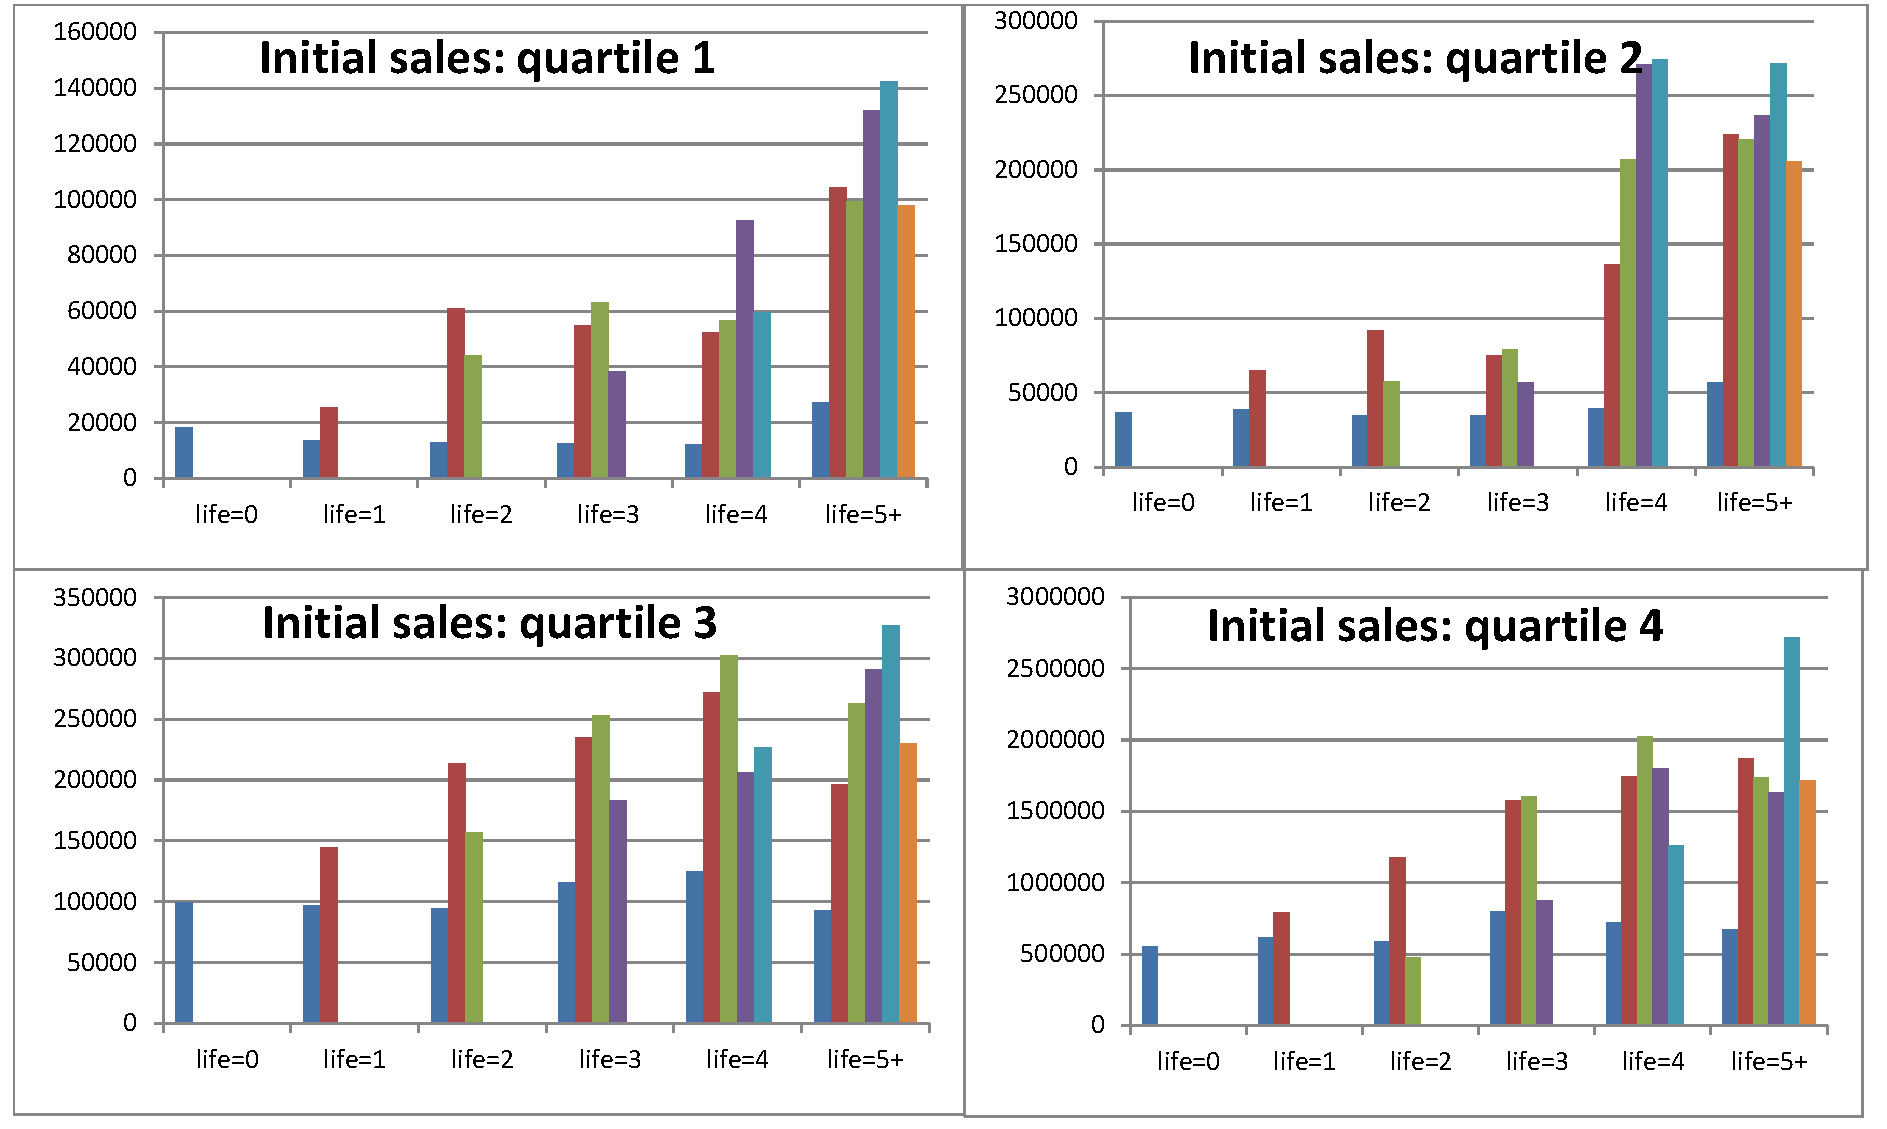
\includegraphics[width=\textwidth]{figures/Figure_1_quadrants_v2.png}
\caption{\textbf{Average annual sales per match, by initial size quartile}}
\label{fig:match_maturation}
\end{figure}
\end{center}

\section{A\ Model of Exporting at the Transactions Level}

We now develop a model of exporter behavior consistent with the patterns
reviewed above. Buyer-seller relationships form and disband at irregular
intervals. Similarly, export shipments are discrete events distributed
unevenly through time. To capture these features of the data, and to allow
agents to update their behavior each time their circumstances change, we
formulate our model in continuous time, treating all of the exogenous
processes in our model as Markov jump processes.

Explaining the evolution of a firm's exports and domestic sales requires
modeling both its sales to existing buyers and the evolution of its
portfolio of clients. We can treat these two components sequentially. We
first consider the relationship between a seller and an individual buyer.
Having characterized the seller's profits from a relationship with an
individual buyer, we then turn to her learning about the popularity of her
product, i.e., the chance that a potential buyers likes her product.
Finally, we characterize her search for buyers.

\subsection{A Seller-Buyer Relationship}

This section characterizes the profit streams that sellers generate from
successful business relationships. The expressions we develop here describe
relationships between domestic firms and foreign buyers, but with
appropriate relabelling of market-wide variables they apply equally to
relationships between domestic firms and domestic buyers.

\subsubsection{Profits from a single shipment}

Several features of our model are standard. First, at any time $t$ seller $j$
can hire workers at a wage $w_{t}$ in real local currency units, each of
whom can produce $\varphi _{j}$ $\in \{\varphi ^{_{1}},..,\varphi
^{_{N_{\varphi }}}\}$ units of output.\footnote{%
We treat $\varphi $ as time-invariant to facilitate model identification.
Other sources of idiosyncratic temporal variation in sales will be discussed
shortly.\medskip} \ Hence seller $j$'s unit cost in local currency is $%
w_{t}/\varphi _{j}.$ If she sells at price $p_{jt}$ in foreign currency her
unit profit in local currency is%
\begin{equation}
p_{jt}/e_{t}-w_{t}/\varphi _{j},  \label{unit profit}
\end{equation}%
where $e_{t}$ is the exchange rate. Second, goods markets are
monopolistically competitive and each producer supplies a unique
differentiated product.

Once buyer $i$ has agreed to form\ a business relationship with seller $j,$
he periodically places sales orders with $j$. For $j$, an order from $i$
that arrives at time $t$ generates revenue:%
\begin{equation}
X_{ijt}=\left( \frac{p_{jt}}{P_{t}}\right) ^{1-\eta }y_{ijt}\overline{X}_{t},
\label{demand}
\end{equation}%
where $\eta >1$ is buyers' elasticity of demand, $p_{jt}$ is the price of
seller $j$'s product, $\overline{X}_{t}$ is the average spending level among
all potential foreign buyers, $P_{t}$ is the relevant price index for all
competing products in the foreign market, and $y_{ijt}\in
\{y^{_{1}},..,y^{_{Ny}}\}$ is a time-varying demand shifter idiosyncratic to
the $ij$ relationship.\footnote{%
Not all buyers necessarily face the same range of goods and hence the same
aggregate price index $P$. We treat idiosyncratic components of the price
index as $P$ as reflected in $y_{ijt}.\medskip $}

For simplicity, and to keep the analysis as close as possible to other
heterogenous firm models, we assume that the seller posts a non-negotiable
price, charging the optimal markup over unit cost:\footnote{%
An alternative specification would introduce bilateral bargaining between
buyer and seller.\medskip}

\begin{equation}
p_{jt}=\frac{\eta }{\eta -1}\frac{e_{t}w_{t}}{\varphi _{j}}  \label{price}
\end{equation}%
By (\ref{unit profit}), (\ref{demand}), and (\ref{price}),\ an order from
buyer $i$ at time $t$ therefore generates the following profits for seller $%
j $:

\begin{equation*}
\pi _{ijt}=\frac{1}{\eta }\frac{\overline{X}_{t}}{e_{t}}\left( \frac{%
e_{t}w_{t}\eta /(\eta -1)}{\varphi _{j}P_{t}}\right) ^{1-\eta }y_{ijt}.
\end{equation*}

We can combine all the macroeconomic variables affecting the profit of any
seller from this source selling in this destination, along with constants,
as:%
\begin{equation*}
x_{t}=\frac{1}{\eta }\frac{\overline{X}_{t}}{e}\left( \frac{e_{t}w_{t}\eta
/(\eta -1)}{P_{t}}\right) ^{1-\eta },
\end{equation*}%
where $x\in \{x^{_{1}},..,x^{_{N_{x}}}\}$ is general to all potential buyers
in the foreign market. Suppressing subscripts on state variables, this
allows us to write the profits from a sale as:

\begin{equation}
\pi _{\varphi }(x,y)=x\varphi ^{\eta -1}y,  \label{profit2}
\end{equation}
\qquad \qquad

In what follows, (\ref{profit2}) is all we take from our specification of
preferences and pricing behavior into the dynamic analysis. Any set of
assumptions that deliver this simple multiplicative expression for a firm's
profit from a sale would serve us equally well.

\subsubsection{Relationship dynamics}

At any point in time, each seller maintains business relationships with an
endogenous number of buyers. These relationships form as a consequence of a
search process that will be characterized in the following section, and they
dissolve for several reasons. First, there is a constant exogenous hazard $%
\delta $ that any particular relationship will terminate, which could be due
to the demise of the buyer or the buyer no longer finding the seller's
product useful. Second, after each sale to a particular buyer, the seller
evaluates whether it is worth sustaining her relationship with him. Doing so
keeps the possibility of future sales to him alive, but it also means paying
the fixed costs $F$ of maintaining the account, providing technical support,
and maintaining client-specific product adjustments.\footnote{%
For instance, Colombian producers of construction materials interviewed for
a related project (Dom\'{\i}nguez et al, 2013) referred that it is frequent
for foreign buyers to request adjustments in the specifications of products
or packages. In turn, these require adjustments in the production process
that are costly to maintain.}

When deciding whether to maintain a particular business relationship, the
seller knows her own type, $\varphi $, the macro state, $x$ and profits from
the current sale, $\pi _{\varphi }(x,y)$ to the buyer in question. She can
therefore infer this buyer's current $y$ value and calculate the value of
her relationship with him to be:%
\begin{equation*}
\widetilde{\pi }_{\varphi }(x,y)=\pi _{\varphi }(x,y)+\max \left\{ \widehat{%
\pi }_{\varphi }(x,y)-F,0\right\} .
\end{equation*}%
Here $\widehat{\pi }_{\varphi }(x,y)$ is the expected value of continuing a
relationship that is currently in state $(x,y).$ Clearly the seller
terminates this relationship if $\widehat{\pi }_{\varphi }(x,y)$ $<F.$

If a seller pays $F$ to keep a relationship active, and if the relationship
does not end anyway for exogenous reasons, one of several events will next
affect it: with hazard $\lambda ^{b}$ the buyer will place another order,
with hazard $q_{xx^{\prime }}^{X}$ $x$ will jump to some new marketwide
state $x^{\prime }\neq x$, or with hazard $q_{yy^{\prime }}^{Y}$ $y$ will
jump to some new buyer-specific shock $y^{\prime }\neq y$.\footnote{%
Since sales in the data are discrete events rather than flows, we model the
buyer's purchases accordingly. We think of the buyer not as making use of
the products continually but in discrete spurts. For example, the buyer
might be a producer of a product that it makes in batches. At the completion
of each batch it buys inputs for the next batch.\medskip} Let $\tau _{b}$ be
the random time that elapses until one of these events occurs. Given that $x$
and $y$ are Markov jump processes, $\tau _{b}$ is distributed exponentially
with parameter $\lambda ^{b}+\lambda _{x}^{X}+\lambda _{y}^{Y}, $ where%
\begin{equation}
\lambda _{x}^{X}=\sum_{x^{\prime }\neq x}q_{xx^{\prime }}^{X}  \label{q_K}
\end{equation}%
and%
\begin{equation}
\lambda _{y}^{Y}=\sum_{y^{\prime }\neq y}q_{yy^{\prime }}^{Y},  \label{q_Y}
\end{equation}%
are the hazards of transiting from $x$ to any $x^{\prime }\neq x,$ and from $%
y$ to any $y^{\prime }\neq y,$ respectively. Then assuming the seller has a
discount factor $\rho ,$ the continuation value $\widehat{\pi }_{\varphi
}(x,y)$ solves the Bellman equation:%
\begin{eqnarray*}
\widehat{\pi }_{\varphi }(x,y) &=&\mathbf{E}_{\tau _{b}}\left[ e^{-(\rho
+\delta )\tau _{b}}\frac{1}{\lambda ^{b}+\lambda _{x}^{X}+\lambda _{y}^{Y}}%
\left( \sum_{x^{\prime }\neq x}q_{xx^{\prime }}^{X}\widehat{\pi }_{\varphi
}(x^{\prime },y)+\sum_{y^{\prime }\neq y}q_{yy^{\prime }}^{Y}\widehat{\pi }%
_{\varphi }(x,y^{\prime })+\lambda ^{b}\widetilde{\pi }_{\varphi
}(x,y)\right) \right] \\
&=&\frac{1}{\rho +\delta +\lambda ^{b}+\lambda _{x}^{X}+\lambda _{y}^{Y}}%
\left( \sum_{x^{\prime }\neq x}q_{xx^{\prime }}^{X}\widehat{\pi }_{\varphi
}(x^{\prime },y)+\sum_{y^{\prime }\neq y}q_{yy^{\prime }}^{Y}\widehat{\pi }%
_{\varphi }(x,y^{\prime })+\lambda ^{b}\widetilde{\pi }_{\varphi
}(x,y)\right)
\end{eqnarray*}

Before a seller has met her next buyer, she does not know what state $y$
this buyer will happen to be in. So when choosing her search intensity for
new business relationships, she must base her decisions on the ex ante
expected pay-off to forming a new business relationship. Given the market
state $x$, a type-$\varphi $ seller calculates this expected value as:%
\begin{equation*}
\widetilde{\pi }_{\varphi }(x)=\sum_{s}\Pr (y^{s})\widetilde{\pi }_{\varphi
}(x,y).
\end{equation*}%
where $\Pr (y^{s})$ is the probability that a randomly selected buyer is
currently in state $y^{s}\in \{y^{_{1}},..,y^{_{Ny}}\}$.\footnote{%
Here we take the probabilities $\Pr (y^{m})$ to be the ergodic distribution
of $y$ implied by the transition hazards $q_{yy^{\prime }}^{Y}.$ We could
assume that the distribution at the time of the first purchase is different
from the ergodic one.\medskip}

For the purposes of the search model that follows, all that matters about an
individual relationship is $\widetilde{\pi }_{\varphi }(x),$ and this object
can be estimated directly from data on the revenue streams generated by
matches. Nonetheless, the history of a seller's interactions with a given
buyer affects its overall sales trajectory and hence matters for our
characterization of aggregate export dynamics.

Hereafter, we will denote the expected value of a relationship with a
foreign buyer by $\widetilde{\pi }_{\varphi }^{f}(x)$ and the expected value
of a relationship with a home market buyer by $\widetilde{\pi }_{\varphi
}^{h}(x).$ These two objects are calculated in the same way, but since
expenditure levels ($\overline{X}_{t}$) and price indices ($P_{t}$) differ
across markets, and no exchange rate factor $e$ is necessary for domestic
profit calculations, each has its own process for the market-wide state
variable, $x.$ These market-wide demand shifters are denoted $x^{f}$ and $%
x^{h}$ below$.$

\subsection{Learning about Product Appeal}

In each market, sellers conduct market-specific searches for buyers. When
searching in market $m\in \{h,f\}$, each recognizes that some fraction $%
\theta ^{m}$ $\in \lbrack 0,1]$ of the potential buyers she meets there will
be willing to do business with her. An encounter with one of these willing
buyers generates an expected profit stream worth $\widetilde{\pi }_{\varphi
,x}^{m}$, while an encounter with any of the remaining potential buyers does
not generate a sale then or subsequently.

Each seller's $\theta ^{h}$ and $\theta ^{f}$ values are drawn before she
has met any clients. These draws remain fixed through time, inducing
permanent cross-market differences in her product's popularity. All $\theta
^{m}$ draws are independently beta-distributed across sellers and markets:%
\begin{equation*}
b(\theta ^{m}|\alpha ,\beta )=\frac{\Gamma (\alpha +\beta )}{\Gamma (\alpha
)\Gamma (\beta )}\left( \theta ^{m}\right) ^{\alpha -1}(1-\theta
^{m})^{\beta -1},\;m\in \{h,f\},
\end{equation*}%
where $\Gamma (\phi )=\int_{0}^{\infty }z^{\phi -1}e^{-z}dz$ is the gamma
function (needed to ensure that the distribution has the proper limits).
However, the independence of $\theta ^{h}$ and $\theta ^{f}$ does not mean
sellers' domestic and foreign sales are likewise independent. Rather,
cross-market correlation in sales will be induced by\ the firm type $\varphi
,$ which can be viewed as capturing aspects of product appeal that are
common to both markets$.$\footnote{%
The firm effect is similarly interpreted to reflect both productive
efficiency and product appeal in Melitz (2003) and many other papers based \
on CES demand systems. However in the present context, the global aspects of
product appeal captured by $\varphi $ are qualitatively distinct from the
market-specific product appeal effects captured by $\theta $. The former
determines the amount of a product each buyer purchases, given that he is
interested, while the latter determines what fraction of potential buyers
are willing to place orders with the seller, should they happen to meet
her.\medskip}

\textbf{Benchmark model:} Sellers are presumed to have already met many
potential customers in the domestic market, and thus to have learned their $%
\theta ^{h}$ draws. But sellers typically have far less experience abroad,
so in the benchmark version of our model, we allow them to still be learning
about their $\theta ^{f}$ draws. Specifically, each seller recognizes that
for any given $\theta ^{f},$ the probability a random sample of $n$
potential foreign buyers will yield $a$ customers is binomially distributed: 
\begin{equation*}
q\left[ a|n,\theta ^{f}\right] =\binom{n}{a}\left[ \theta ^{f}\right] ^{a}%
\left[ 1-\theta ^{f}\right] ^{n-a}.
\end{equation*}%
So after she has met $n^{f}$ potential buyers abroad, $a^{f}$ of whom were
willing to buy her product, a seller's posterior beliefs about her $\theta
^{f}$ draw are distributed:%
\begin{equation*}
p(\theta ^{f}|a^{f},n^{f})\propto q\left[ a^{f}|n^{f},\theta ^{f}\right]
\cdot b(\theta ^{f}|\alpha ,\beta )
\end{equation*}%
where the factor of proportionality is the inverse of the integral of the
right-hand side over the support of $\theta ^{f}$. Since the beta
distribution is the conjugate prior for the binomial, a firm's expected
success rate after $a$ successes in $n$ trials has a convenient closed-form
representation: 
\begin{equation}
\overline{\theta }_{a,n}^{f}=E\left[ \theta ^{f}|a^{f},n^{f}\right]
=\int_{0}^{1}\theta p(\theta |a^{f},n^{f})d\theta =\frac{a^{f}+\alpha }{%
n^{f}+\alpha +\beta }.  \label{success_probability}
\end{equation}%
This posterior mean converges to $p\lim \left( \frac{a^{f}}{n^{f}}\right)
=\theta ^{f}$ as $n$ gets large.

\textbf{No-learning model: }As an alternative to our benchmark model, we
consider the possibility that sellers already know their product's
popularity in \textit{both} markets, so that $p(\theta ^{f}|a^{f},n^{f})$ is
a degenerate distribution and $\overline{\theta }_{a,n}^{f}=$ $\theta ^{f}.$
In this version of the model, sellers' matching histories only affect their
search intensities by affecting their visibility in each market, as we will
discuss shortly. Our no-learning model is not nested by the benchmark model,
it is simply a different characterization of the role of information in
driving search policies.\footnote{%
In order for the learning model to nest the no learning model, each firm
would have to have its own Beta distribution parameters, $\alpha $ and $%
\beta .$}

\subsection{Searching for Buyers}

To complete our characterization of firms' behavior, we now consider
sellers' search intensities in each market. Each seller continuously chooses
the market-specific hazard $s^{m},$ $m\in \{h,f\},$ with which she
encounters a potential buyer, recognizing that this involves the
instantaneous flow cost $c^{m}(s^{m},a^{m}),$ where $c^{m}(s^{m},a^{m})$ is
increasing and convex in $s^{m}.$\footnote{%
Interviews conducted with Colombian exporters revealed a variety of
activities firms pursue to meet potential buyers abroad (Dom\'{\i}nguez, et
al, 2013). Ranked roughly in terms of decreasing cost, these included
maintaining a foreign sales office; paying the exports promotion office to
organize visits with prospective clients abroad, and sending their sales
representatives to those visits; sending sales representatives abroad to
visit potential clients on their own; attending trade fairs; paying a
researcher to search the web for foreign firms that purchase products
similar to their own; paying browsers to ensure that their site appear near
the top of a search for their product type; maintaining a web site in
English. Interviewees also reported that relatively low-cost activities,
such as traveling to trade fairs, or translating their websites to English,
led to relationships with one or two clients every few years. Establishing a
larger network of clients required much more costly activities.} Whether $%
c^{m}(s^{m},a^{m})$ increases or decreases in the number of successful
matches, $a^{m},$ depends upon the relative strength of several forces and
will be left for the data to determine. Costs might fall with $a^{m}$
because encounters with interested buyers increase the seller's visibility
and enhance her opportunities to meet additional potential buyers.
Alternatively, costs might rise if the pool of easy-to-reach buyers becomes
"fished out," as in Arkolakis\ (2007).

We can now describe optimal search behavior, beginning with the foreign
market. Recall that when the foreign market state is $x^{f}$, a type-$%
\varphi $ seller expects the value of a new business relationship will be $%
\widetilde{\pi }_{\varphi }^{f}(x^{f}).$ Further, she believes the next
match will yield such a relationship with probability $\overline{\theta }%
_{a,n}^{f}$. Combined with search cost function $c^{f}(s^{f},a^{f})$ and the
jump process for $x^{f}$, these objects imply sellers' optimal search policy
abroad.

To characterize this policy, let $\tau _{s}^{f}$ be the random time interval
until the next foreign search event, which could be either a change in the
marketwide state $x^{f}$ or an encounter with a potential buyer. Then,
suppressing market superscripts, the optimal search intensity $s$\ for a
type-$\varphi $ firm with foreign market search history $(a,n)$ solves the
following the Bellman equation:%
\begin{eqnarray*}
&&V_{\varphi }(a,n,x)=\max_{s}\mathbf{E}_{\tau _{s}}\left[
-c(s,a)\int_{0}^{\tau _{s}}e^{-\rho t}dt+\frac{e^{-\rho \tau _{s}}}{%
s+\lambda _{x}^{X}}\cdot \left( \sum_{x^{\prime }\neq x}q_{xx^{\prime
}}^{X}V_{\varphi ,}(a,n,x^{\prime })\right. \right. \\
\; &&\left. \left. 
\begin{array}{c}
\; \\ 
\;%
\end{array}%
+s\left[ \overline{\theta }_{a,n}(\widetilde{\pi }_{\varphi }(x)+V_{\varphi
}(a+1,n+1,x)+(1-\overline{\theta }_{a,n})V_{\varphi }(a,n+1,x)\right]
\right) \right]
\end{eqnarray*}%
(Recall that $\lambda _{x}^{X}$ is given by (\ref{q_K}).) Taking
expectations over $\tau _{s}$ yields:%
\begin{eqnarray}
V_{\varphi }(a,n,x) &=&\max_{s}\frac{1}{\rho +s+\lambda _{x}^{X}}\left[
-c(s,a)+\sum_{x^{\prime }\neq x}q_{xx^{\prime }}^{X}V_{\varphi
,}(a,n,x^{\prime })\right.  \label{V_search2} \\
&&\left. 
\begin{array}{c}
\; \\ 
\;%
\end{array}%
+s\left\{ \overline{\theta }_{a,n}\left[ \widetilde{\pi }_{\varphi
}(x)+V_{\varphi }(a+1,n+1,x)\right] +(1-\overline{\theta }_{a,n})V_{\varphi
}(a,n+1,x)\right\} \right]  \notag
\end{eqnarray}%
Applying the multiplication rule for differentiation and using expression (%
\ref{V_search2}) for $V_{\varphi }(a,n,x)$, the optimal search intensity $%
s^{\ast }$ satisfies:%
\begin{equation}
\frac{\partial c(s^{\ast },a)}{\partial s}=\overline{\theta }_{a,n}\left[ 
\widetilde{\pi }_{\varphi }(x)+V_{\varphi }(a+1,n+1,x)\right] +(1-\overline{%
\theta }_{a,n})V_{\varphi }(a,n+1,x)-V_{\varphi }(a,n,x)
\label{FOC_MS_learning}
\end{equation}%
That is, the marginal cost of search must equal the expected marginal
benefit of a match, which includes the expected value of the associated
profit stream, $\overline{\theta }_{a,n}\widetilde{\pi }_{\varphi }(x)$, and
the expected value of the information generated.

Now consider the home market. Since we assume sellers have already learned
their true success rates at home, $\theta _{j}^{h},$ new encounters do not
influence expectations, and we need not condition the value function or the
expected success rate on search histories$.$ Again suppressing market
superscripts, the Bellman equation collapses to:%
\begin{eqnarray}
V_{\varphi }(x,a) &=&\max_{s}\frac{1}{\rho +\lambda _{x}^{X}}\left[
-c(s,a)+\sum_{x^{\prime }\neq x}q_{xx^{\prime }}^{X}V_{\varphi }(x^{\prime
},a)\right.  \notag \\
&&\left. 
\begin{array}{c}
\; \\ 
\;%
\end{array}%
+s\left\{ \theta _{j}^{h}\left[ \widetilde{\pi }_{\varphi }(x)+V_{\varphi
}(a+1,x)\right] +(1-\theta _{j}^{h})V_{\varphi }(a,x)\right\} \right]
\end{eqnarray}%
and the first-order condition is simply:%
\begin{equation*}
\frac{\partial c(s^{\ast },a)}{\partial s}=\theta _{j}^{h}\left[ \widetilde{%
\pi }_{\varphi }(x)+V_{\varphi }(a+1,x)-V_{\varphi }(a,x)\right] .
\end{equation*}%
The marginal cost of search equals the expected profit from a successful
relationship times the probability of success. Of course, this condition
also describes foreign market search in the no-learning version of the model.

\section{An empirical version of the model}

\subsection{The search cost function}

To implement our model empirically, we impose additional structure in
several respects. First, we specify a functional form for our search cost
function. Generalizing Arkolakis\ (2007) to allow for network effects, we
write these costs as:%
\begin{equation}
c^{m}(s^{m},a^{m})=\kappa _{0}^{m}\frac{\left[ (1+s^{m})\right] ^{\kappa
_{1}}-1}{\kappa _{1}\left[ 1+\ln (1+a^{m})\right] ^{\gamma }}.
\label{cost of effort}
\end{equation}%
where $m\in \{h,f\}.$ Several properties of this function merit note. First,
marginal costs fall at a rate determined by $\gamma $ with the number of
successful matches a seller has already\ made, so $\gamma >0$ implies
\textquotedblleft network\textquotedblright\ effects and $\gamma <0$ implies
"congestion" effects.\footnote{%
To contain the dimensionality of the computational problem we solve, we
assume that firms with more than $a^{\ast }$ buyers have (i) exhausted their
learning effects, and (ii) reap no additional network effects at the margin
from further matches. We choose $a^{\ast }$ to exeed the observed maximum $a$
for 99 percent of sellers in the foreign (United States) market. Also, we
set $a=a^{\ast }$ for all sellers in their home (Colombian) market.\medskip}
Second, a seller who is not searching in a particular market incurs no
search cost: $c^{m}(0,a^{m})=0.$ Third, given the cumulative number of
successful matches, $a,$ the marginal cost of search increases with $s$ at a
rate determined by $\kappa _{1}:$ $\frac{\partial c^{m}(s^{m},a^{m})}{%
\partial s^{m}}$ $=$ $\kappa _{0}^{m}(1+s^{m})^{\kappa _{1}-1}/\left[ 1+\ln
(1+a)\right] ^{\gamma }.$ Fourth, we allow the cost function scalar to vary
across markets, since the cost of maintaining any given level of visibility
is likely to be higher in foreign markets. Finally, since $a^{m}$ is the
cumulative number of successes in market $m$, network effects endure, even
if a firm is not actively searching.

\subsection{Processes for exogenous state variables}

Next we impose more structure on the exogenous state variables, $\varphi ,$ $%
x^{h},$ $x^{f},$ $y^{h}$ and $y^{f}.$ All are assumed to have zero means in
logs, and the net effect of these normalizations is undone by introducing
scalars $\Pi ^{h}$ and $\Pi ^{f}$ into the home and foreign profit
functions, respectively:%
\begin{eqnarray}
\pi _{\varphi }^{f}(x^{f},y^{f}) &=&\Pi ^{f}x^{f}\varphi ^{\eta -1}y^{f},
\label{profit3_f} \\
\pi _{\varphi }^{h}(x^{h},y^{h}) &=&\Pi ^{h}x^{f}\varphi ^{\eta -1}y^{f}
\label{profit3_h}
\end{eqnarray}

More substantively, we impose that the cross-firm distribution of $\varphi $
is log normal with variance parameter $\sigma _{\varphi },$ and we treat all
of the Markov jump processes $(x^{h},y^{h},x^{f},y^{f})$ as independent
Ehrenfest diffusion processes. The idiosyncratic match shocks, $y^{f}$ and $%
y^{h},$ are assumed to share the same distribution, but we allow the $x^{f}$
and $x^{h}$ processes to differ. Among other things, the latter accommodates
the fact that the exchange rate affects aggregate demand and price indices
in the two markets differently.

Any variable $z$ generated by an Ehrenfest process can be discretized into $%
2g+1$ possible values, $g\in I^{+}:$ $z\in \{-g\Delta ,$ $-(g-1)\Delta ,$ $%
..,$ $0,..,$ $(g-1)\Delta ,$ $g\Delta \}.$ Further, it jumps to a new value
with hazard $\lambda _{z},$ and given that a jump occurs, it goes to $%
z^{\prime }$ according to:

\begin{equation*}
z^{\prime }=\left\{ 
\begin{array}{c}
z+\Delta \\ 
z-\Delta \\ 
\text{other}%
\end{array}%
\right. \text{with probability }\left\{ 
\begin{array}{c}
\frac{1}{2}\left( 1-\frac{z}{g\bigtriangleup }\right) \\ 
\frac{1}{2}\left( 1+\frac{z}{g\bigtriangleup }\right) \\ 
0%
\end{array}%
\right. .
\end{equation*}%
Thus, given a grid size $g$, the intensity matrices $Q^{X}=\left\{
q_{ij}^{X}\right\} _{i,j=1,N^{X}}$ and $Q^{Y}=\left\{ q_{ij}^{Y}\right\}
_{i,j=1,N^{Y}}$ that were introduced in section 3.1 are each block-diagonal
and characterized by a single parameter, $\Delta $.

\section{Estimation}

\subsection{Stage 1: estimating observable jump processes}

Shimer (2005) shows that if $z$ follows a continuous time Ehrenfest
diffusion process, it asymptotes to an Ornstein-Uhlenbeck process with mean
zero as the fineness of the grid increases:\footnote{%
Specifically, replacing the parameter vector $(\lambda ,g,\Delta )$ with $%
(\lambda /\epsilon ,g/\epsilon ,\Delta \sqrt{\epsilon }),$ $\epsilon >0,$
leaves the autocorrelation parameter $\mu $ and the instantaneous variance
parameter $\sigma $ unchanged. But as $\epsilon \rightarrow 0,$ the
innovation $dW$ $\ $approaches normal.\medskip} 
\begin{equation*}
dz=-\mu zdt+\sigma dW.
\end{equation*}%
Here $\mu =\lambda _{z}/g$, $\sigma =\sqrt{\lambda _{z}}\Delta $, and $W$
follows a Weiner process. Accordingly, since it is possible to observe
proxies for $x^{f}$ and $x^{h}$, these can be viewed as discrete time
observations on underlying Ornstein-Uhlenbeck processes, and the parameters
of these processes can be econometrically estimated. Then, given $\mu $ and $%
\sigma ,$ estimates of $\Delta $ and $\lambda $ for these processes can be
inferred.

\begin{table}[tbp]
\caption{\textbf{Market-wide Demand Shifters}}
\label{tab:dem_shift}\centering
\begin{tabular}{lll}
\multicolumn{3}{c}{} \\ \hline\hline
& \textit{Parameter} & \textit{value} \\ \hline
home macro state jump hazard & $\lambda ^{x_{h}}$ & \multicolumn{1}{c}{1.200}
\\ 
foreign macro state jump hazard & $\lambda ^{x_{f}}$ & \multicolumn{1}{c}{
1.215} \\ 
home macro state jump size & $\Delta ^{x_{h}}$ & \multicolumn{1}{c}{0.003}
\\ 
foreign macro state jump size & $\Delta ^{x_{f}}$ & \multicolumn{1}{c}{0.053}
\\ \hline
\end{tabular}%
%
%
%
%
%
%
%
%
%
%
%
%
%
%
%
%
%
%
%
%
%
%
%
%
%
%
%
%
%
%
%
%
%
%
%
%
%
%
%
%
%
%
%
%
%
%
%\caption{\textbf{Market-wide Demand Shifters}}
\end{table}

Measuring $x^{f}$ as real expenditures on manufacturing goods in the U.S.,
and measuring $x^{h}$ as real expenditures on manufacturing goods in
Colombia, we obtain the results reported in Table \ref{tab:dem_shift}.%
\footnote{%
Our foreign market size mesaure is the OECD time series on American GDP in
'Industry, including energy' adding imports and subtracting net exports of
manufactures. Our home market size measure is real Colombian expenditures on
manufacturing goods, taken from DANE. We converted all of the data used for
the estimation into real 1992 US dollars, deflating nominal US dollars with
the consumer price index available on the US Bureau of Labor Statistic
website. We used an official Colombian Peso - US Dollar exchange rate time
series downloaded from the Central Bank of Colombia to convert Pesos to
nominal US Dollars} They imply that $x^{f}$ and $x^{h}$ both jump 1.2 times
per year, on average. However, jumps in the U.S. market tend to be much
larger, essentially because they reflect movements in the real exchange rate
as well as movement in dollar-denominated expenditures.

\label{sec:indirect_inference}

\subsection{Stage 2: Indirect inference}

\FloatBarrier

Our data are relatively uninformative about the rate of time discount $\rho $
and the demand elasticity $\eta $, so we do not attempt to estimate either
one$.$ For the former we follow convention and assume $\rho =0.05$. For the
latter, following many previous trade papers, we fix the demand elasticity
at $\eta =5.$ Also, to limit the size of the estimated parameter vector, we
take the exogenous match failure rate to be the observed match failure rate
among matches at least 3 years old ($\delta =0.326$), we take the search
cost function to be quadratic in search intensity (${\small \kappa _{1}}=2$%
), and we assume that the hazard rate for the buyer is once per quarter ($%
\lambda _{y}=4$).\footnote{%
These last three parameters could in principle be estimated, and in earlier
drafts we have done so. However, they have not appeared to be
well-identified.}

All of the remaining parameters we estimate jointly using the transactions
data summarized in Section \ref{sec:data} above. These parameters include
the market size scalars (${\small \Pi }^{h},{\small \Pi }^{f.}$), the fixed
costs of maintaining a match ($F^{h},F^{f}$), the parameters of the product
appeal distributions (${\small \alpha }{\small ,}{\small \beta }$), the
dispersion of the productivity distribution ($\sigma _{\varphi }$), the jump
size for the idiosyncratic buyer shocks ($,\Delta _{y}$), the hazard rate
for shipments (${\small \lambda }_{b}$), the network/congestion parameter ($%
\gamma $), and the market-specific cost function scaling parameters ($%
{\small \kappa _{0}^{h},}$ ${\small \kappa _{0}^{f}}$). \textbf{\ }For
notational convenience we collect these parameters in the vector $\Lambda :$%
\begin{equation*}
\Lambda =\left( {\small \Pi }^{h},{\small \Pi }^{f.},F^{h},F^{f},{\small %
\alpha },{\small \beta },\sigma _{\varphi },\Delta _{y},{\small \lambda }%
_{b},{\small \gamma ,\kappa _{0}^{h},\kappa _{0}^{f}}\right)
\end{equation*}

We construct our estimator for $\Lambda $ using the method of indirect
inference (Gouri\'{e}roux and Monfort, 1996). That is, for each candidate $%
\Lambda $ vector$,$ we use the model to simulate the foreign and domestic
transactions of an artificial sample of producers. Then, using these
simulated data, we estimate a set of reduced-form regressions that summarize
the relationships we want our model to capture. \ Finally, looking across
candidate $\Lambda $ vectors, we choose the one that makes the regression
coefficients from simulated data correspond as closely as possible to the
corresponding regression coefficients based on sample data. Algebraically,
our estimator is 
\begin{equation*}
\hat{\Lambda}=\min_{\Lambda }\left[ \bar{m}-m(\Lambda )\right] ^{\prime }W%
\left[ \bar{m}-m(\Lambda )\right] ,
\end{equation*}%
where $\bar{m}$ is a column vector of regression coefficients obtained from
sample data, $m(\Lambda )$ is the analogous vector of regression
coefficients based on data simulated at $\Lambda ,$ and $W$ is a compatible
non-singular weighting matrix. Setting $W^{-1}=var(\bar{m}-m(\Lambda ))$
maximizes the efficiency of this estimator, but any non-singular $W$ will
yield consistent estimates. We use a block-diagonal version of $var(\bar{m}%
-m(\Lambda )),$ with each block corresponding to the moments from a
particular regression.

The regressions themselves are reported in Tables \ref{tab:haz_reg}, \ref%
{tab:client_dist} and \ref{tab:hf_sales}. In each table, the data-based
regression estimates are reported, and their standard errors are reported
below them in parentheses. To facilitate comparisons between the sample and
the simulated data, and with no loss of information, we have replaced the
intercept of each regression with the mean value of the dependent variable
in cases where that was possible.\footnote{%
Several regressions were done in real pesos within the Colombian national
statistical agency (DANE). We are not confident that they can be expressed
in units that are strictly comparable to the real dollar units in which U.S.
customs records were expressed.} We now briefly describe these regressions
and our reasoning in choosing them.

\textbf{Search policy}. The first regression in Table \ref{tab:haz_reg}
summarizes the effects of firms' market experiences on their search
intensity ($s$). Roughly speaking, this equation can be viewed as a second
order approximation to the foreign market policy function (\ref%
{FOC_MS_learning})--a central object in our model. The dependent variable is
a proxy for a firm's foreign market search intensity after $n$ successful
matches, namely, the inverse of the time interval between firm $j$'s $n^{th}$
and $n+1^{st}$ match. And the right-hand side is a second-order translog
function of this firm's cumulative number of successes ($a$) and cumuluative
success rate ($\frac{a}{n}$)$.$ To deal with firms that have had no
successes, we add 1 to $a$ and to $\frac{a}{n}$ before taking logs.

The unit of observation here is an exporter-specific new match, and we
define a new match to occur whenever an exporter makes a shipment to a buyer
it has not dealt with before. We view this first shipment as a sample of the
exporter's merchandise, so we only consider this match to be successful if
it results in at least one additional shipment. This interpetation of the
data means we can use customs records to directly infer the cumulative
number of successes for each firm $j$ ($a_{nj}$) after each of its $n\in
\{1,...,N_{j}\}$ matches, and the associated cumulative success rates $(%
\frac{a}{n})_{nj}$.

Interpreting the coefficient estimates for this regression is problematic,
both because it\ includes second order terms and because we have not
controlled for the highly nonlinear firm effects generated by $\varphi $ and 
$\theta ^{f}.$\ But evaluation of this equation on a grid of success rates
and cumulative successes gives us a crude sense for the relationships
implied by our estimates. The results (available upon request) show that
search intensity is sensitivity to success rates, but it strongly increases
with cumulative successes.

\textbf{Separation policy. }Equation ($ii$) captures a second basic feature
of firms' exporting behavior: match termination policies. Here the unit of
observation is seller $j$'s $i^{th}$ match in year $t$, and the dependent
variable, $D^{exit\text{ }match},$ takes a value of unity when this match is
in its final year.\footnote{%
Only active matches are included in the sample.} Our model implies that
matches are more likely to terminate when the idiosyncratic demand shock $%
z_{ijt}$ and/or the firm's productivity level $\varphi _{j}$ is low. Neither
variable is directly observable, so we use several of their correlates as
explanatory variables: current match sales, $X_{ijt}^{f}$, age of the match, 
$A_{ijt}$, and export market tenure, $\Delta _{ijt}$. All variables are
expressed in logs and, given the patterns revealed by Table \ref%
{tab:sep_rates}, we allow firms in their first year of exporting ($D^{new%
\text{ }to\text{ }mkt}=1$) to experience particularly high failure rates.%
\footnote{%
Note, however, that in Table \ref{tab:client_dist}, matches that die after a
single shipment are treated as having existed for less than one year, while
our model-based estimates treat these cases of single shipments as
unsuccessful meetings that did not lead to business relationships.}

Equation ($ii$) helps to identify the fixed costs of maintaining an
established foreign match, $F^{f}$. That is, conditioning on sales, $%
X_{ijt}^{f},$ matches are more likely to survive when fixed costs are low.
Failure rates are also affected by the volatility of $z_{ijt},$ which is
governed by the jump size, $\lambda _{y}.$

Not surprisingly, estimates of equation ($ii$) reflect the same patterns
that we noted in connection with Table \ref{tab:client_dist}. Matches in
their first year are relatively likely to fail, as are matches that start
with relatively small sales volumes. The results also show that exporters
with more experience in foreign markets tend to have longer-lived
relationships, a feature of the data that our model captures with cross-firm
variation in productivity levels, $\varphi $.

\textbf{Match success rates} The remaining regressions in Table \ref%
{tab:sep_rates} concern the distribution of success rates, $\theta $.
Equation ($iii$) summarizes the average success rate among active exporters
and its relation to the cumulative number of meetings an exporter has had ($%
n $). Accordingly it is informative about $\alpha /(\alpha +\beta )$ and
selection due to learning. Equation $(iv)$ describes dispersion in success
rates--i.e., the squared residuals from equation ($iii$)--among exporters
with different experience ($n$) levels. Both regressions suggest that
selection takes place as firms acquire market tenure, since success rates
are higher among experienced (high-$n$) firms, and the dispersion in success
rates among such firms is lower.

\textbf{Client distributions and shipment frequencies}. The next set of
regressions appears in Table \ref{tab:client_dist}. Equation ($v$)
summarizes the information on client distributions in Table \ref%
{tab:erg_cli_dist}. Specifically, letting $\Phi (\ell )$ be the fraction of
exporters with no more than $\ell $ active clients, column ($v$) reports the
regression of $\ln (1-\Phi (\ell ))$ on $\ln \ell $ and $\left( \ln \ell
\right) ^{2}.$\footnote{%
By construction, the intercept of the (non-parametric version of) this
regression \ line must be zero.} We choose this functional form because
earlier studies have found that exporters' foreign client distributions are
approximately Pareto, implying that the relationship between $\ln (1-\Phi
(\ell ))$ and $\ln \ell $ is approximately linear. Note that our data
confirm a nearly-Pareto client distribution, as the coefficient on the
quadratic term is quite small (-0.055).

Equation $(v)$ helps to identify the cost function parameters ($\kappa
_{0}^{h},\kappa _{0}^{f},\gamma $) because the client distribution largely
reflects firms' search intensities. In particular, the network effects
captured by the parameter $\gamma $ determine how much of a search cost
discount large (big $a$) firms enjoy, and thus the "fatness" of the
right-hand tail of the client distribution $\Phi (\cdot ).$

Equation ($vi$), the other regression in Table \ref{tab:client_dist}, simply
establishes the mean log number of shipments per year per continuing match.
It serves as a target for the shipment arrival hazard and obviously helps to
identify $\lambda _{b}.$

\textbf{Match- and firm-level sales} Regressions that characterize the time
series properties of firms' exports, cross-firm dispersion in exports, and
patterns of correlation between exports and domestic sales are collected in
Table \ref{tab:hf_sales}. These equations are particularly informative about
the parameters $\left( {\small \Pi }^{h},{\small \Pi }^{f.},F^{h},F^{f},%
\sigma _{\varphi },\Delta _{y}\right) .$ Equation ($vii$) is an AR1 in log
match revenues, conditioned on match age and a dummy to control for
first-year effects. By the logic reviewed in section 5.1 above, the root
(0.826) and root mean square error (1.208) in this AR1 identify the jump
size, $\Delta _{y}$ and the cross-firm variance in productivity, $\sigma
_{\varphi },$ up to selection effects. Also, together with equation ($ii$),
the mean log annual revenue per match (10.67) essentially pins down the
profit function scalar and the fixed cost of maintaining a foreign match ($%
\Pi _{f},F^{f})$.

The last four equations in Table \ref{tab:hf_sales} involve domestic sales.
Since we don't observe firms' individual matches in the domestic market,
these regressions describe establishment-level panel data merged with
Colombian customs records.\footnote{%
More precisely, regressions ($viii$) through ($x$) in Table \ref%
{tab:hf_sales} are done using a combination of the Colombian Annual
Manufacturing Survey (AMS) and Colombian administrative records of exports
transactions. The data used cover 1993-2007. Exports are merged into the AMS
using firm identifiers. This is done because the AMS has no export
information for 1993-1999, and because the dynamics of aggregate exports
reported in the EAM starting in 2004 differ substantially from aggregate
reports from other sources.} Equations ($viii$) is an AR1 for home sales,
and is thus informative about the extent which firms adjust their domestic
connections and their associated match specific sales in response to
idiosyncratic shocks. Accordingly, the coefficients in this equation are
particularly helpful in identifying $\kappa _{0}^{h}$ and $F^{h},$ and the
mean squared error helps identify $\sigma _{\varphi }$ and $\alpha /(\alpha
+\beta )$. Equation ($ix$) is a simple projection of firm level exports on
firm-level domestic sales. It serves to distinguish market-specific
variation in revenues from variation in revenues that is common to both
markets. Thus the estimated parameters of this equation, including its mean
squared error, are informative about the variance of productivity shocks ($%
\sigma _{\varphi }^{2})$, which are common to both markets, relative to the
variance of market-specific appeal draws, $\theta ^{h}$ and $\theta ^{f}$.%
\footnote{%
Given the average success rate, $\alpha /(\alpha +\beta )$, the variances of 
$\theta ^{h}$ and $\theta ^{f}$depend only on $\alpha +\beta $.}

\FloatBarrier

\begin{table}[tbp]
\caption{\textbf{Match hazards, success rates, and endurance}}
\label{tab:haz_reg}{\small \ }\centering
\par
{\small 
\begin{tabular}{lllll}
\hline\hline
& $(i)$ & $(ii)$ & $(iii)$ & $(iv)$ \\ 
& $\ln (\lambda _{ij})$ & $D_{ijt}^{exit\text{ }match}$ & $\frac{a_{ij}}{%
n_{ij}}$ & $u_{a_{ij}/n_{ij}}^{2}$ \\ \hline
mean, dep. variable & $%
\begin{array}{c}
\text{-0.719} \\ 
\text{(0.621e-2)} \\ 
\end{array}%
$ & $%
\begin{array}{c}
\text{0.395} \\ 
\text{(0.319e-2)} \\ 
\end{array}%
$ & $%
\begin{array}{c}
\text{0.413} \\ 
\text{(0.153e-2)} \\ 
\end{array}%
$ & $%
\begin{array}{c}
\text{0.091} \\ 
\text{(0.26e-3)} \\ 
\end{array}%
$ \\ 
$\ln (1+a_{ij})$ & \ \ \ \ \ \ -- & \ \ \ \ \ \ -- & $%
\begin{array}{c}
\text{0.093 } \\ 
\text{(0.003)} \\ 
\end{array}%
$ & $%
\begin{array}{c}
\text{-0.056} \\ 
\text{(0.000)} \\ 
\end{array}%
$ \\ 
$\ln (1+n_{ij})^{2}$ & $%
\begin{array}{c}
\text{-0.818} \\ 
\text{(0.113)} \\ 
\end{array}%
$ & \ \ \ \ \ \ -- & \ \ \ \ \ \ -- & \ \ \ \ \ \ -- \\ 
$\left[ \ln (1+a_{ij})\right] ^{2}$ & $%
\begin{array}{c}
\text{0.312} \\ 
\text{(0.017)\ } \\ 
\end{array}%
$ & \ \ \ \ \ \ -- & \ \ \ \ \ \ -- & \ \ \ \ \ \ -- \\ 
$\ln (1+\frac{a_{ij}}{n_{ij}})$ & $%
\begin{array}{c}
\text{-1.132} \\ 
\text{(0.296)} \\ 
\end{array}%
$ & \ \ \ \ \ \ -- & \ \ \ \ \ \ -- & \ \ \ \ \ \ -- \\ 
$\left[ \ln (1+\frac{a}{n})\right] ^{2}$ & $%
\begin{array}{c}
\text{2.451} \\ 
\text{(0.396)} \\ 
\end{array}%
$ & \ \ \ \ \ \ -- & \ \ \ \ \ \ -- & \ \ \ \ \ \ -- \\ 
$\ln (1+a_{ij})\cdot \ln (1+\frac{a_{ij}}{n_{ij}})$ & $%
\begin{array}{c}
\text{-0.708} \\ 
\text{(0.134)} \\ 
\end{array}%
$ & \ \ \ \ \ \ -- & \ \ \ \ \ \ -- & \ \ \ \ \ \ -- \\ 
$D_{ijt}^{new\text{ }to\text{ }mkt}$ & \ \ \ \ \ \ -- & $%
\begin{array}{c}
\text{0.034} \\ 
\text{(0.011)} \\ 
\end{array}%
$ & \ \ \ \ \ \ -- & \ \ \ \ \ \ -- \\ 
$\ln X_{ijt}^{f}$ & \ \ \ \ \ \ -- & $%
\begin{array}{c}
\text{-0.031} \\ 
\text{(0.002)} \\ 
\end{array}%
$ & \ \ \ \ \ \ -- & \ \ \ \ \ \ -- \\ 
$\ln A_{ijt}$ & \ \ \ \ \ \ -- & $%
\begin{array}{c}
\text{-0.054} \\ 
\text{(0.009)} \\ 
\end{array}%
$ & \ \ \ \ \ \ -- & \ \ \ \ \ \ -- \\ 
$\ln \Delta _{jt}$ & \ \ \ \ \ \ -- & $%
\begin{array}{c}
\text{-0.028} \\ 
\text{(0.007)} \\ 
\end{array}%
$ & \ \ \ \ \ \ -- & \ \ \ \ \ \ -- \\ \hline
observations (rounded) & 38,500 & 23,500 & 35,800 & 35,800 \\ \hline
\end{tabular}
}\endcenter
\par
\begin{tablenotes}
\item \textbf{Notes:} Unit of observation, columns $i$,  $iii$ and $iv$: seller $ j$'s $i^{th}$ match. Unit of observation, column $ii$: seller $ j$'s $i^{th}$ match in its $t^{th}$ year. $\lambda_{ij}=$ inverse of time interval between commencement of match $i$ and commencement of the next one for exporter $j$ $D_{ijt}^{exit match}=1$ if exporter $j^{\prime }s$ $i^{th}$ match dies in year $t$. $a_{ij} $ = cumulative number of successes for exporter $j$ at time of match $i$. $D_{ijt}^{new to mkt}=1$ if exporter $j^{\prime }s$ $i^{th}$ match is in its first year. $\ln A_{ijt}=$ log age of exporter $j^{\prime }s$ $i^{th}$  match. $\ln \Delta_{jt} =$ log age of exporter $j$ in year $t$. $X_{ijt}^{f}$ $=$ foreign sales volume generated by exporter $j^{\prime }s$ $i^{th}$ match.
\end{tablenotes}
\end{table}

\begin{table}[tbp]
\caption{\textbf{Client distribution and shipment frequency}}\centering
{\small \ }
\par
{\small 
\begin{tabular}{lll}
\hline\hline
& $(v)$ & $(vi)$ \\ 
& $\ln (1-\Phi (\ell ))$ & $\ln (s_{ijt})$ \\ \hline
mean, dep. variable & $%
\begin{array}{c}
\text{-5.973} \\ 
\text{(2.173)}%
\end{array}%
$ & $%
\begin{array}{c}
\text{0.971 } \\ 
\text{(0.004)}%
\end{array}%
$ \\ 
$\ln (\ell )$ & $%
\begin{array}{c}
\text{-1.8813 } \\ 
\text{(0.1123)}%
\end{array}%
$ & - \\ 
$(\ln \ell )^{2}$ & $%
\begin{array}{c}
\text{-0.0545 } \\ 
\text{(0.0211)}%
\end{array}%
$ & - \\ \hline
sample restrictions & $\ell >0$ & $s_{ijt}>0$ \\ 
observations & 43 & 87,000 \\ \hline
\end{tabular}
} \endcenter%
\begin{tablenotes}
\item \textbf{Notes:} $\ell$: number of active clients;  $\Phi ( ) = $ cumulative distribution of exporters in terms of  $\ell$;
$s_{ijt}=$ number of shipments per year to client $i$ by exporter $j$ in year $t$
\end{tablenotes}
\label{tab:client_dist}
\end{table}

\begin{table}[tbp]
\caption{\textbf{Home and foreign sales regressions}}\centering
{\small \ }
\par
{\small 
\begin{tabular}{llllll}
\hline\hline
& $(vii)$ & $(viii)$ & $(ix)$ & $(x)$ & $(xi)$ \\ 
& $\ln X_{ijt}^{f}$ & $\ln X_{jt}^{h}$ & $\ln X_{jt}^{f}$ & $D_{jt}^{f}$ & $%
\frac{X_{jt}^{f}}{X_{jt}^{f}+X_{jt}^{h}}$ \\ \hline
mean, dep. variable & $%
\begin{array}{c}
\text{10.665 } \\ 
\text{(0.002)} \\ 
\end{array}%
$ & $%
\begin{array}{c}
\text{--} \\ 
\text{{}} \\ 
\end{array}%
$ & $%
\begin{array}{c}
\text{-- } \\ 
\text{{}} \\ 
\end{array}%
$ & $%
\begin{array}{c}
\text{0.102} \\ 
\text{(0.003)} \\ 
\end{array}%
$ & $%
\begin{array}{c}
\text{0.127} \\ 
\text{(0.002)} \\ 
\end{array}%
$ \\ 
$R_{ijt-1}$ & $%
\begin{array}{c}
\text{0.328} \\ 
\text{(0.018)} \\ 
\end{array}%
$ & - & - & - & - \\ 
$\ln X_{ijt-1}^{f}$ & $%
\begin{array}{c}
\text{0.826 } \\ 
\text{(0.004)} \\ 
\end{array}%
$ & - & - & - & - \\ 
$\ln X_{jt-1}^{h}$ & - & $%
\begin{array}{c}
\text{0.976} \\ 
\text{(0.029)} \\ 
\end{array}%
$ & - & - & - \\ 
$\ln X_{jt}^{h}$ & - & - & $%
\begin{array}{c}
\text{0.323} \\ 
\text{(0.110)} \\ 
\end{array}%
$ & - & - \\ 
$\ln \Delta _{t}$ & $%
\begin{array}{c}
\text{0.063} \\ 
\text{(0.014)} \\ 
\end{array}%
$ & - & - & - & - \\ 
root mse & 1.2079 & 0.4621 & 2.1665 & 0.303 & 0.243 \\ \hline
sample restrictions & $X_{ijt}^{f},X_{ijt-1}^{f}>0$ & $%
X_{jt}^{h},X_{jt-1}^{h}>0$ & $X_{jt}^{f},X_{jt}^{h}>0$ & $X_{jt}^{h}>0$ & $%
X_{jt}^{f},X_{jt}^{h}>0$ \\ 
observations & 25,400 & 99,300 & 11,600 & 119,800 & 12,500 \\ \hline
\end{tabular}
} \endcenter%
\begin{tablenotes}
\item \textbf{Notes:} $R_{ijt}=1$ if exporter $j^{\prime }s$ $i^{th}$ match is in its first
year. $\ln \Delta{jt} =$ log age of exporter $j$. $X_{ijt}^{f}$ $=$ foreign sales volume generated by exporter $j^{\prime }s$ $i^{th}$ match. $X_{jt}^{f}$ $=$ total foreign sales volume generated by firm $j$. $X_{jt}^{h}$ $=$ total home sales volume generated by firm $j$. $D_{jt}^{f}$ $=$ 1 if firm $j$ is an exporter.
\end{tablenotes}
\label{tab:hf_sales}
\end{table}

\FloatBarrier

Finally, equations ($x$) and ($xi$) describe the relative importance of home
versus foreign sales. The former gives the share of firms that participate
in the foreign market and thereby speaks to the relative return to
maintaining foreign versus domestic business connections, that is $(\Pi
^{f}, $ $F^{f},\kappa _{0}^{f})$ versus $(\Pi ^{h},$ $F^{h},\kappa _{0}^{h})$%
. The latter gives the average share of exports to the U.S. in total sales
of exporting firms. Accordingly, it largely reflects the number of clients
in each market, and thus responds especially to differences between $\kappa
_{0}^{f}$ and $\kappa _{0}^{h}.$

\textbf{Sensitivity analysis }As suggested by Andrews et al. (2017), we
check which moments are important using the sample analog to the matrix $%
(G^{\prime }WG)^{-1}G^{\prime }W$ \ where $G=\frac{-\partial \left[
m(\Lambda )\right] }{\partial \Lambda ^{\prime }}$ is the Jacobian for the
vector of simulated moments. "Intuitively, this matrix is a local
approximation to the mapping from moments to estimated parameters."
(Andrews, et al., 2017, p. 1555) Evaluated at our benchmark estimates (to be
discussed), we obtain the results reported in detail in Appendix \ref%
{sec:sensitivity}. Here we summarize the patterns that emerge.

First, most parameters respond to many moments rather than one or several.
Limiting our attention to elasticities with absolute value greater than 0.1,
most parameters show significant responses to at least 5 moments, and
several ($F^{f},$ $F^{h},\gamma )$ respond to more than 15. All parameters
respond to at least 2. The moments that affect the most parameters are those
generated by the match sales autogression (equation $vii$), the shipping
rate regression (equation $vi$), the domestic sales autoregression (equation 
$viii$), the regression explaining the variance in success rates (equation $%
iv$), and the fraction of firms that export (equation $x$).\linebreak

\subsection{Parameter estimates}

Table \ref{tab:struct_param} reports estimates of the structural parameter
vector $\Lambda $ for both the benchmark and the no-learning model. Although
our estimator exploits month-to-month transitions in the customs records,
all hazards are normalized so that the unit of time is one year. Thus, for
example, our estimate of $\delta $ implies that on average, matches last
roughly 4 months (one-third of a year) before separating for exogenous
reasons. Most parameter estimates are similar for both models, though, as
we'll argue below, the benchmark model fits the data better. We therefore
focus our discussion on the results for this model, turning later to the
main distinguishing features of the no-learning results.

\textbf{Benchmark parameter estimates} Active matches generate an average of 
$\lambda _{b}=15.43$ shipments per year, and the profits associated with
these shipments vary widely across firms and macro conditions. Evaluating
the gross profit-per-shipment functions (\ref{profit3_f}) and (\ref%
{profit3_h}) at our estimated values for $\Pi ^{h}$, $\Pi ^{f}$ and the
parameters governing realizations for $\varphi ,$ $x,$ and $y$, we find that
gross profits per shipment (before fixed costs) for a firm at the median
productivity level matched to a median buyer are essentially zero.
Accordingly, these firms are not active. On the other hand, a firm with
productivity 1.9 standard deviations above the mean earns gross profits per
shipment ranging from \textbf{\$}US 4 to \$US 42, depending upon what state
its buyer is in. In the domestic market, the analogous figures range from 
\textbf{\$}US 45 to \$US 405\textbf{.} Further, a firm with the highest
productivity matched to the best possible buyer in the most favorable macro
state earns \textbf{\$}US\textbf{\ }31,512 in gross profits per export
shipment and \textbf{\$}US\textbf{\ }281,570 in profit per domestic
shipment. Of course, firms almost never attain these maxima, and when they
do they are very unlikely to repeat their performance. This is consequence
of the short expected life span of matches, and the fact that buyers'
demands change an average of $\lambda _{y}=4$ times per year.

These seemingly small magnitude of these figures reflects several factors.
First, the productivity distribution for exporting firms come from the
right-hand tail of the unconditional productivity distribution. Thus those
firms with productivity 1.9 standard deviations above the mean unconditional
mean of $\varphi $ are actually the smaller exporters. Second, since
revenues per shipment are $\eta =5$ times profits per shipment, and since an
average of $\lambda _{b}=15.43$ shipment occur per year, expected annual
revenues from a match that survives the entire year are $\eta \cdot \lambda
_{b}=77.15$ times as large as profits per shipment for that match.

Turning to the fixed cost estimates, note that both are quite small ($F^{f}$%
\textbf{=}\$0.30\textbf{, }$F^{h}$\textbf{=}\$0.03). These costs thus have
no affect on major exporters. Nonetheless, they affect the fraction of
exporting firms by keeping fringe players that would otherwise sell tiny
amounts out of foreign markets.

The profit and cost function scalars are much more important. The model
assigns lower search costs to the home market ($\kappa _{0}^{h}=859.0$
versus $\kappa _{0}^{f}=3,079.7$) and much larger profits per sale ($\Pi
^{h}/\Pi ^{f}=\exp \left( -3.88-6.16\right) =9.77$). Both patterns help
explain the small amount of output exported to the U.S. among these firms
(Table \ref{tab:hf_sales}, regression $xi$). And the two sets of scalars are
separately identified by their different effects on match arrival rates
(Table \ref{tab:sep_rates}, regression $i$) and revenues from ongoing
matches (Table \ref{tab:hf_sales}, regressions $vii$ and $viii$). The
benchmark model also implies that search costs fall significantly as firms
acquire market visibility through successful matches ($\gamma =0.383$). As
mentioned earlier, identification of this visibility effect comes largely
from the shape of the client distribution (Table \ref{tab:client_dist},
regression $v$).

So what are the costs of making new matches? For a firm with no prior
successful matches in the foreign market, a search intensity sufficient to
yield an average of one new match per year costs $c^{f}(1,0)=$ \textbf{\$}US 
$1,539$, but an expected yield of four new matches---about one successful
match for a firm with average product appeal---costs $c^{f}(4,0)=$ \$US $%
24,637$. The analogous figures in the home market are $c^{h}(1,0)=$ \$US $%
428 $ and $c^{h}(4,0)=$ \$US $6,848$. But having an established reputation
is helpful. A firm that has already made 2 successful foreign matches could
expect to pay only $c^{f}(4,2)=$ \textbf{\$}US $20,142$ for the next
one---roughly 20 percent less than the cost of the first one. Similarly, a
firm that has already made two successful home market matches could expect
to pay $c^{h}(4,2)=$ \$US $5,598$ for the third. These reputation effects
are nontrivial, and other things equal, they create a cost advantage for
well-established firms.

Given match payoffs and search costs, firms' search intensity is determined
by their expected success rates. Their (unobserved) actual rates are drawn
from a beta distribution, which we estimate to have mean $\alpha /(\alpha
+\beta )=0.23$ and standard deviation $\sqrt{\alpha \beta /\left[ (\alpha
+\beta )^{2}(\alpha +\beta +1)\right] }=$ $0.23$. Hence, before they acquire
export market experience, firms expect that roughly 1 in 4 new encounters
with potential buyers will lead to business relationships. And since new
exporters are uncertain about their $\theta ^{f}$ draws, they expect to
learn a good deal from the outcomes of their early matches.\ 

\begin{table}[tbp]
\caption{\textbf{Structural parameter estimates}}\centering
{\small \ }
\par
{\small 
\begin{tabular}{llrrrr}
\hline\hline
&  & \multicolumn{2}{r}{Benchmark model \ \ \ } & \multicolumn{2}{r}{
No-learning model} \\ 
& \textit{Parameter} & \textit{value} & \textit{std. error} & \textit{value}
& \textit{std. error} \\ \cline{2-3}\cline{2-6}
log of domestic profit scalar & $\ln \Pi ^{h}$ & -3.879 & (0.1364) \ \  & 
-3.460 & (0.0725) \\ 
log of foreign profit scalar & $\ln \Pi ^{f}$ & -6.135 & (0.1993) \ \  & 
-6.273 & (0.0759) \\ 
fixed cost, domestic & $F^{h}$ & 0.027 & (0.0047) \ \  & 0.037 & (0.0064) \\ 
fixed cost, foreign & $F^{f}$ & 0.296 & (0.0428) \ \  & 0.301 & (0.0359) \\ 
First $\theta $ distribution parameter & $\alpha $ & 0.571 & (0.0454) \ \  & 
0.581 & (0.0703) \\ 
Second $\theta $ distribution parameter & $\beta $ & 1.894 & (0.2320) \ \  & 
4.661 & (0.2107) \\ 
demand shock jump size & $\Delta ^{y}$ & 1.882 & (0.2222) \ \  & 1.951 & 
(0.1810) \\ 
shipment order arrival hazard & $\lambda _{b}$ & 15.426 & (0.1991) \ \  & 
15.431 & (0.1428) \\ 
std. deviation, log firm type & $\sigma _{\varphi }$ & 1.386 & (0.0095) \ \ 
& 1.401 & (0.0051) \\ 
network effect parameter & $\gamma $ & 0.383 & (0.0485) \ \  & 0.508 & 
(0.0479) \\ 
log of home search cost scalar & $\ln \kappa _{0}^{h}$ & 11.722 & (0.1486) \
\  & 12.480 & (0.0850) \\ 
log of foreign search cost scalar & $\ln \kappa _{0}^{f}$ & 13.002 & 
(0.0095) \ \  & 13.666 & (0.1373) \\ \cline{3-6}
log of fit metric & $\ln (\Lambda )$ & \multicolumn{2}{r}{10.806 \ \ \ \ \ \
\ \ \ \ \ } & \multicolumn{2}{r}{11.346 \ \ \ \ \ \ \ \ \ } \\ \hline
\end{tabular}
}
\label{tab:struct_param}
\end{table}

\textbf{No-learning parameter estimates }Recall that our no-learning model
differs from the benchmark model in that it presumes each firm $j$ already
knows the fraction of the foreign population of buyers that is willing to do
business with it, $\theta _{j}^{f}.$ This assumption implies that low-appeal
firms never bother to invest much in foreign market searches. Further,
compared to firms that learn their $\theta _{j}^{f}$ draws through
experience, fully-informed firms have less incentive to search intensively
when they are new to export markets. That is, for these firms their is no
information value to matches.

The last two columns of Table \ref{tab:struct_param} present parameter
estimates based on this version of the model. Most parameters are similar,
but for the no-learning model the estimate of the network effect is larger ($%
\gamma =0.50$ versus $\gamma =0.38$) and the estimates of search costs are
higher  ($\kappa _{0}^{h}=859$ and $\kappa _{0}^{f}=3,079$ versus $\kappa
_{0}^{h}=1,826$ and $\kappa _{0}^{f}=5,982$).\ Higher search cost scalars
and larger network effects appear to help the no-learning model explain the
observed pattern of small entry, gradual growth, and eventual dominance by
high-$\theta $ entrants without relying on learning effects. However, the
no-learning version of the model does substantially worse than the benchmark
version according to Rivers and Vuong's (2002) test statistic for non-nested
comparisons.\footnote{%
The Rivers and Voung (2002) statistic takes the form $T_{n}=\frac{\sqrt{n}}{%
\hat{\sigma}_{n}}\left[ \hat{\Lambda}^{1}-\hat{\Lambda}^{2}\right] ,$ where $%
\hat{\Lambda}^{1}$ and $\hat{\Lambda}^{2}$ are the MSM fit metrics for the
two models, and $\hat{\sigma}_{n}^{2}$ approximates $var\left[ \hat{\Lambda}%
^{1}-\hat{\Lambda}^{2}\right] .$ This statistic has a standard normal
distribution under the null $E(\hat{\Lambda}^{1})=E(\hat{\Lambda}^{2}).$
Applying it to our context, and treating the weighting matrix $W$ as
non-stochastic when calculating $\hat{\sigma}_{n}^{2}$, we get $T_{n}=$
-1,583.2. Two caveats apply. First, it is not obvious what the right sample
size $n$ is in our context, given that some of our moments are constructed
using firm-year level data, some are constructed using shipment-level, and
some are constructed using match level. We used a very conservative
approximation to the number of firms we base our inferences on ($n=1000$),
but clearly, the test statistic would have been highly significant at much
smaller values. Second, this test statistic does not recognize randomness in
the fit statistics due to the simulation draws we use. Time and hardware
limitations prevented us from using samples so large that this was
negligible, though we used common seeds for both sets of results.}

\section{Analysis of results}

\subsection{Model fit}

Appendix \ref{sec:model_fit} juxtaposes the data-based moments, $\bar{m},$
with their simulated counterparts, $m(\Lambda ),$ from the benchmark model.
Generally, the patterns in the data are replicated by our model, though not
all of the model-based equation estimates correspond closely to their
data-based counterparts. In particular, average exporting rates,
match-specific sales dynamics, and the client distribution are well-captured
by the model, as are most mean values of dependent variables. However the
model fails to generate the association between success rates and firms'
search intensities that we observe in the data. This relationship is
relatively weak---note the large standard errors for the coefficients on $%
\ln (1+\frac{a}{n})$ and $\left[ \ln (1+\frac{a}{n})\right] ^{2}$ in column
1 of Table \ref{tab:haz_reg}---so it doesn't receive much weight in the fit
metric. A more detailed summary of the fit can be found in Appendix \ref%
{sec:model_fit}.

Since we have not targeted the patterns described in Section \ref{sec:data}
when estimating, it is instructive to ask how well they are replicated by
our model. Tables \ref{tab:brooks_compare}, \ref{tab:match_exit_compare} and %
\ref{tab:client_dist_compare}\ below provide answers. In the top panel of
table \ref{tab:brooks_compare}, the information in Tables \ref{tab:Brooks}-%
\ref{tab:erg_cli_dist} is collapsed by averaging across exporting cohorts
for which we observe at least 10 years of data. (These cohorts were born in
the years 1997 through 2002.) Recall that values of each aggregate for
2-year olds, 3-year olds, and so on are expressed as fractions of the
corresponding values for 1-year olds. For example, the data tell us that, on
average, only 29 percent of the exporters who began exporting in year t were
still exporting in year t+1, and only 5 percent of those that began
exporting in year t were present in year t+9. \ Likewise, among Colombian
exporters that survive in the U.S. market for 10 years, average exports per
firm are 6.58 times as large as they are among exporters that are in their
first year of exporting.

The bottom panel of Table \ref{tab:brooks_compare} shows corresponding
figures based on model-simulated data. Qualitatively, the patterns in the
actual and the simulated data match up. For both data sets, the largest
drops in the number of exporters occur during the first two years,
thereafter cohort size drops gradually. Likewise, total exports rise early
in cohort's life, and decline thereafter. Finally, exports per surviving
firm grow rapidly over time, reflecting both the exit of small-scale firms
and client accumulation among survivors. It should be noted, however, that
the "average exports" and "total exports" series based on actual data vary
less dramatically with cohort age than the simulated data. Also, in the
data-based figures, the drop in cohort membership is more dramatic during
the first year. In sigifnicant part, these discrepancies reflect the fact
that the data-based figures were constructed by treating the first shipment
between a buyer and a seller as establishing a match, while the model does
not.\footnote{%
Specifically, since the data-based series count single-shipment buyer-seller
encounters as matches, these series inflate the one-year-old firm and total
export counts, while depressing mean exports among one-year olds. And the
one-year old figures appear in the denominator of the ratios for all other
years. Restrictions on data access have temporarily prevented us from
re-doing these tables in a fully compatible way. The issue will be addressed
in a future draft.}

\begin{table}[tbp]
\caption{\textbf{Cohort evolutions: data vs. model}}
\label{tab:brooks_compare}\centering
{\small \ }
\par
{\small 
\begin{tabular}{llll}
\hline\hline
& \multicolumn{3}{l}{\ \ \ \ \ \ \ \ \ \ \ \ \ \textbf{Actual data}} \\ 
\cline{2-4}
Cohort age & Exporters & Total Exports & Average Exports \\ \hline
1 year & 1 & 1 & 1 \\ 
2 years & 0.29 & 1.11 & 3.77 \\ 
3 years & 0.18 & 0.93 & 5.03 \\ 
4 years & 0.14 & 0.67 & 4.66 \\ 
5 years & 0.12 & 0.63 & 5.18 \\ 
6 years & 0.10 & 0.51 & 4.99 \\ 
7 years & 0.08 & 0.50 & 5.72 \\ 
8 years & 0.08 & 0.45 & 5.91 \\ 
9 years & 0.07 & 0.39 & 5.58 \\ 
10 years & 0.06 & 0.40 & 6.58 \\ 
&  &  &  \\ 
&  &  &  \\ 
& \multicolumn{3}{l}{\ \ \ \ \ \ \ \ \ \ \ \ \textbf{Simulated data}} \\ 
\cline{2-4}
Cohort age & Exporters & Total Exports & Average Exports \\ \hline
1 year & 1.00 & 1.00 & 1.00 \\ 
2 year & 0.61 & 1.73 & 2.84 \\ 
3 years & 0.35 & 1.34 & 3.81 \\ 
4 years & 0.19 & 1.81 & 9.50 \\ 
5 years & 0.10 & 2.29 & 22.74 \\ 
6 years & 0.06 & 2.12 & 34.43 \\ 
7 years & 0.05 & 1.89 & 39.69 \\ 
8 years & 0.04 & 1.69 & 43.23 \\ 
9 years & 0.03 & 1.89 & 63.69 \\ 
10 years & 0.02 & 1.46 & 65.17 \\ \hline
\end{tabular}
}
\par
{\endcenter
\begin{tablenotes}
%\bigskip
\item \textbf{Notes:} Figures for cohorts aged 2-10 are expressed relative to corresponding figures for one-year-old cohorts.
\end{tablenotes}
}
\end{table}

\begin{table}[tbp]
\caption{\textbf{Match separation rates}}
\label{tab:match_exit_compare}\centering
{\small \ }
\par
{\small 
\begin{tabular}{lllll}
\hline\hline
& \multicolumn{4}{l}{\ \ \ \ \ \ \ \ \ \ \ \ \ \ \ \ \textbf{Actual data}}
\\ \cline{2-5}
Match age & Quartile 1 & Quartile 2 & Quartile 3 & Quartile 4 \\ \hline
1 year & 82.9 & 75.6 & 67.7 & 52.1 \\ 
2 years & 63.2 & 58.4 & 52.1 & 44.5 \\ 
3 years & 57.3 & 49.4 & 44.6 & 40.3 \\ 
4 years & 55 & 46.8 & 40.8 & 39.2 \\ 
5+ years & 49.7 & 43.7 & 37.6 & 36.7 \\ 
&  &  &  &  \\ 
& \multicolumn{4}{l}{\ \ \ \ \ \ \ \ \ \ \ \ \ \ \ \textbf{Simulated data}}
\\ \cline{2-5}
Match age & Quartile 1 & Quartile 2 & Quartile 3 & Quartile 4 \\ \hline
1 year & 0.60 & 0.88 & 0.89 & 0.63 \\ 
2 years & 0.27 & 0.29 & 0.31 & 0.27 \\ 
3 years & 0.30 & 0.32 & 0.33 & 0.30 \\ 
4 years & 0.31 & 0.28 & 0.20 & 0.32 \\ 
5+ years & 0.28 & 0.30 & 0.36 & 0.36 \\ \hline
\end{tabular}
}
\par
{\endcenter%
\begin{tablenotes}
%\bigskip
\item \textbf{Notes:} Figrures are percentages of the exporters in each age-initial size category that do not export during the following year.
\end{tablenotes}}
\end{table}

\begin{table}[tbp]
\caption{\textbf{Exporter distribution by number of buyers}}
%\begin{table}[tbp]
\centering
{\small \ }
\par
{\small %\begin{table}[]
}
\par
{\small 
\begin{tabular}{lll}
\hline\hline
& \multicolumn{2}{l}{\ \ \ \ \ \ share of exporters} \\ \cline{2-3}
Number of buyers & actual data & simulated data \\ \hline
1 & 0.79 & 0.77 \\ 
2 & 0.11 & 0.10 \\ 
3 & 0.03 & 0.05 \\ 
4 & 0.02 & 0.03 \\ 
5 & 0.01 & 0.02 \\ 
6-10 & 0.02 & 0.03 \\ 
11+ & 0.02 & 0.01 \\ \hline
\end{tabular}
}
\par
{\endcenter%
\begin{tablenotes}
\item \textbf{Notes:} Figures give the ergodic distribution of current buyer counts across exporting firms.
\end{tablenotes}} %\end{table}
\label{tab:client_dist_compare}
\end{table}
%\end{center}

Table \ref{tab:match_exit_compare} compares the match exit rates observed in
the actual data with those observed in the simulated data. These are broken
down by match age, and by the size of the match's first-year sales. As with
the figures in Table \ref{tab:haz_reg}, this comparison is imperfect because
of the differences in the way matches are defined in the two data sets.
Nonetheless, the relatively high failure rates among first-year matches are
replicated by the model, as is the tendency for matches that begin from the
largest sales quartile to fail less frequently than others.\textit{\ }%
However, the high failure rates are concentrated among one-year-old matches
in the simulated data, while they decline more more gradually with age in
the actual data.\textit{\ }Also, unlike the actual data, the exporters that
begin in the smallest size quartile exhibit failure rates as low as those of
the largest exporters\textit{.}

Finally, Table \ref{tab:client_dist_compare} reports the distribution of
client counts across exporters in the actual versus simulated data. Overall
the two distributions match up very well, though the actual data contain
more exporters with two clients (and fewer with more than two clients) than
the model predicts.

\subsection{The value of relationships}

\subsubsection{The value of clients}

In addition to convex search costs, two forces in our model make exporting
decisions forward looking. First, each successful business relationship
improves an exporter's visibility and reduces its cost of finding additional
potential clients. We call this the "network effect." Second, each
match--successful or unsuccessful--conveys information about the scope of
the market for the exporter's product. We call this the "learning effect."
With Bayesian updating (equation \ref{success_probability}), it means that
early matches generate particularly valuable signals and may be worth
pursuing even if they are not expected to generate significant earnings. It
also means that two firms, \textit{ex ante} identical, may have very
different long term experiences in export markets, depending upon whether
their early matches happened to yield successful business relationships.

%\begin{figure}
%    \centering
%    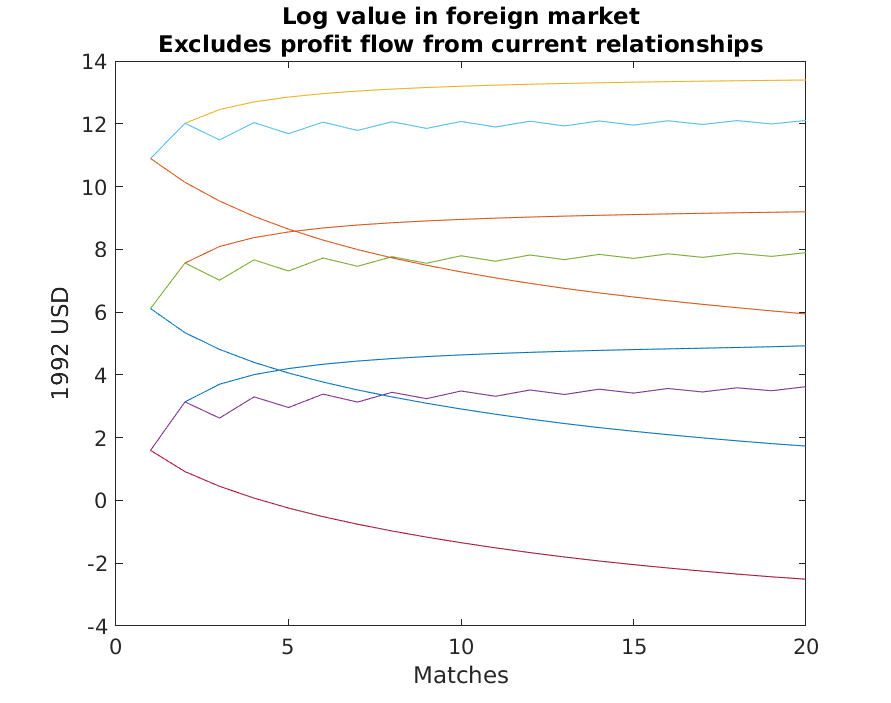
\includegraphics[scale=0.5]{figures/val_f_three_types}
%    \caption{Log continuation value of firms conditional on match history}
%    \label{fig:val_three_types}
%    \caption*{Notes: Continuation value trajectories for firms with productivity in the 10th, 50th, and 90th percentiles of the simulated productivity distribution of exporters.  For each productivity type, we plot values for all successful matches, alternating success and failure, and all failures.}
%\end{figure} 

To get some sense for the combined importance of the network effect and the
learning effect, Figure \ref{fig:val_three_types} shows the perceived change
in the firm's value with each additional meeting. These changes are
exclusive of the profits generated by the new matches, so they describe the
impact of each new match on continuation values solely through these two
effects. We plot the continuation values for firms of three productivity
types, taken from the 10th, 50th, and 90th productivity percentiles among
simulated exporters.\footnote{%
Of course, since low-productivity firms do not export, these are percentiles
of a truncated distribution.} These values depend upon firms' priors
concerning their popularity ($\bar{\theta}^{f}$), which in turn depend upon
the number of meetings ($n$) they have already experienced at the of time
each increment to $a$. (They do not depend upon firms' \textit{true} success
rates, $\theta ^{f},$ as these are unobservable.) We demonstrate this
dependence of perceived continuation values on match histories by
considering several extreme cases: an unbroken string of successful matches (%
$n=a$) and an unbroken string of failures ($n=0$). To provide a benchmark,
we also graph the evolution of firms' values when they experience a strictly
alternating succession of successes and failures ($n\approx 2a)$.

Initial continuation values of the three productivity types of exporters
vary widely. The foreign operations of the highest productivity type of firm
are valued at US\$ 53,800 before its first foreign match, while the median
productivity firm's foreign operations are valued at only US\$ 452 before
its first match, and the foreign operations of the lowest productivity firm
are initially worth only US\$ 5.

The first match has the biggest impact on continuation values, and most of
the impact of additional information has dissipated by the twentieth match.
For example, if its first match is a success, the highest productivity
firm's value jumps to US\$ 165,000. On the other hand, failures quickly
erase firm value. The continuation value of the median productivity firm
with four successful matches is almost the same as the value of the high
productivity firm with four failed matches, at US\$ 5,669.

%\begin{figure}
%    \centering
%    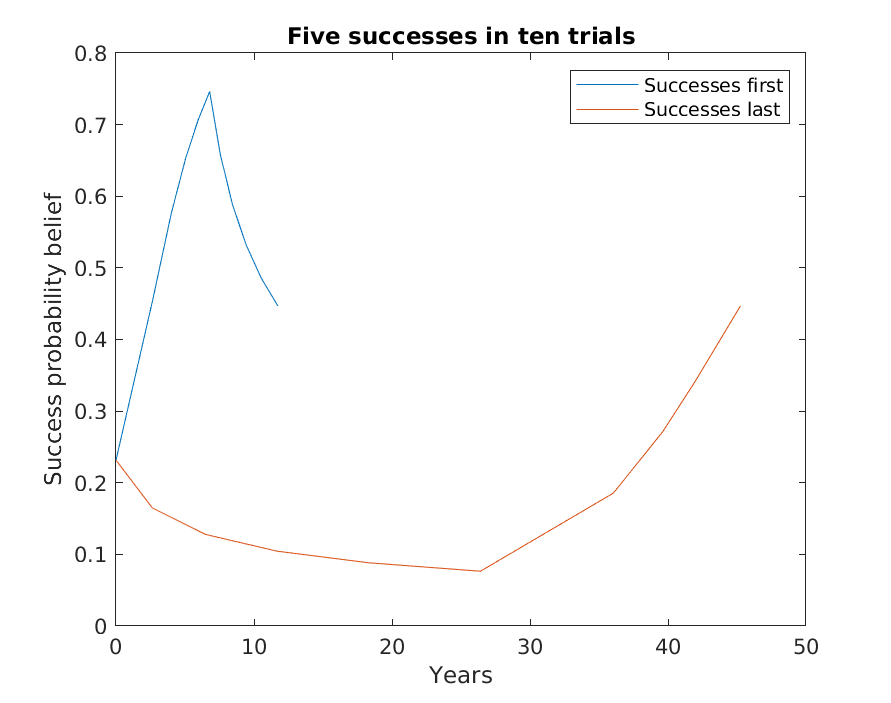
\includegraphics[scale=0.5]{figures/success_beliefs}
%    \caption{Evolution of success probability belief}
%    \label{fig:success_beliefs}
%    \caption*{\small{Notes: Beliefs of a firm with productivity in the 90th percentile of exporters over success probability.  Top line is five success followed by five failures.  Bottom line is five failures followed by five successes.}}
%\end{figure}

In addition to continuation values, match histories affect the intensity
with which firms search for new clients. We explore this dependence in
Figure \ref{fig:success_beliefs}, which plots beliefs regarding $\theta ^{f}$
over time for a firm in the 90th percentile of productivity. Here we assume
that if a firm is searching with intensity $\lambda $, it meets its next
match at exactly the mean waiting time $1/\lambda $. There are two lines on
the plot, both containing five successes and five failures. The only
difference is that in the top line, the successes come first, while in the
bottom line the failures come first. Before any meetings, the beliefs are
the same, and after all 10 meetings they are the same as well because at
this point both histories contain 5 successes.

The key message of Figure \ref{fig:success_beliefs} is that if the successes
come first, it takes 10.5 years to get 10 matches. But if the failures come
first, it takes more than 43 years. Thus, simply because of luck, it takes
four times longer for the failure-first firm to get to 10 meetings and it
searches far less intensively along the way.

\subsubsection{Comparison with no-learning}

%
%\begin{figure}
%    \centering
%    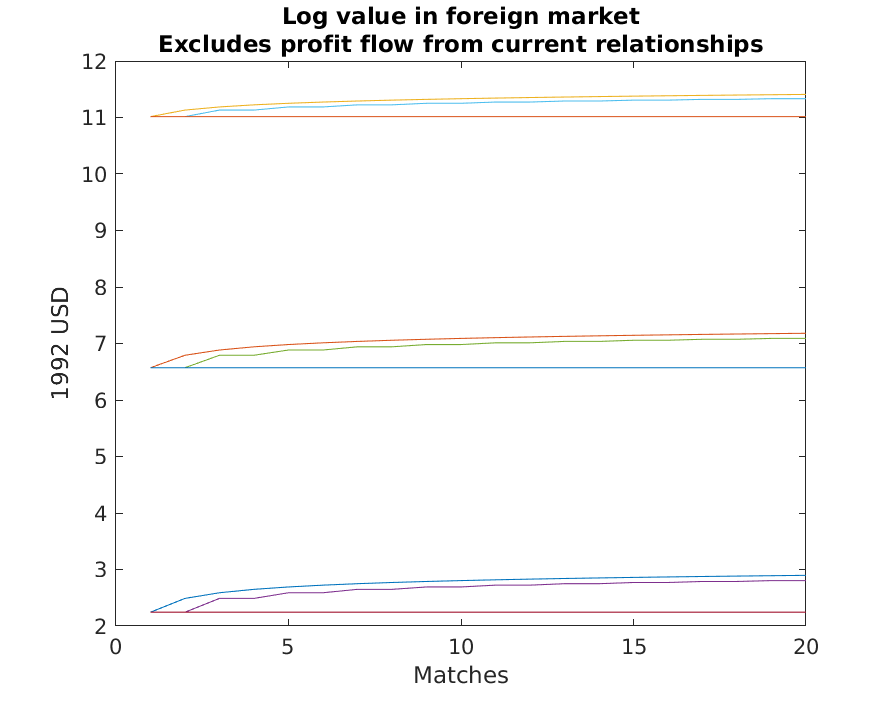
\includegraphics[scale=0.5]{figures/val_f_three_types_nl}
%    \caption{Log continuation value of firms conditional on match history, no learning}
%    \label{fig:val_three_types_nl}
%    \caption*{Notes: Continuation value trajectories for firms with productivity in the 10th, 50th, and 90th percentiles of the simulated productivity distribution of exporters in the learning version of the model.  For each productivity type, we plot values for all successful matches, alternating success and failure, and all failures.}
%\end{figure}

The patterns we have depicted thus far reflect both the network effect and
the learning effect. To gauge their relative importance, we now redo Figure %
\ref{fig:val_three_types} under the assumption that firms know their true $%
\theta ^{f}$ realizations from the start. More precisely, using our
estimates of the "no learning" policy function (see Table \ref%
{tab:struct_param}), we simulate the continuation values of firms at the
10th, 50th, and 90th productivity percentiles. And as in Figure \ref%
{fig:val_three_types} we consider three alternative match histories: only
successes, only failures, and alternating successes and failures. Also,
since true success rates now affect behavior, we give all firms a success
probability of $\theta ^{f}=0.43$. This number corresponds to the 65th
percentile of success probabilities among active exporters in our simulated
data. We chose this particular value because it is close to 50\%, and it is
one of the discritized points on the grid we use for estimation.

The results appear in Figure \ref{fig:val_three_types_nl}. Overall,
continuation values move much less as firms acquire experience, implying
that the new exporter dynamics in Figure \ref{fig:val_three_types} were
mainly due to firms learning their types. Continue values do still rise a
bit when firms make successful matches because these matches make is easier
to meet additional buyers (the "network effect"). However, unsuccessful
matches now have no effect on these values.

%\begin{figure}
%    \centering
%    \begin{subfigure}[b]{0.5\textwidth}
%        \centering
%        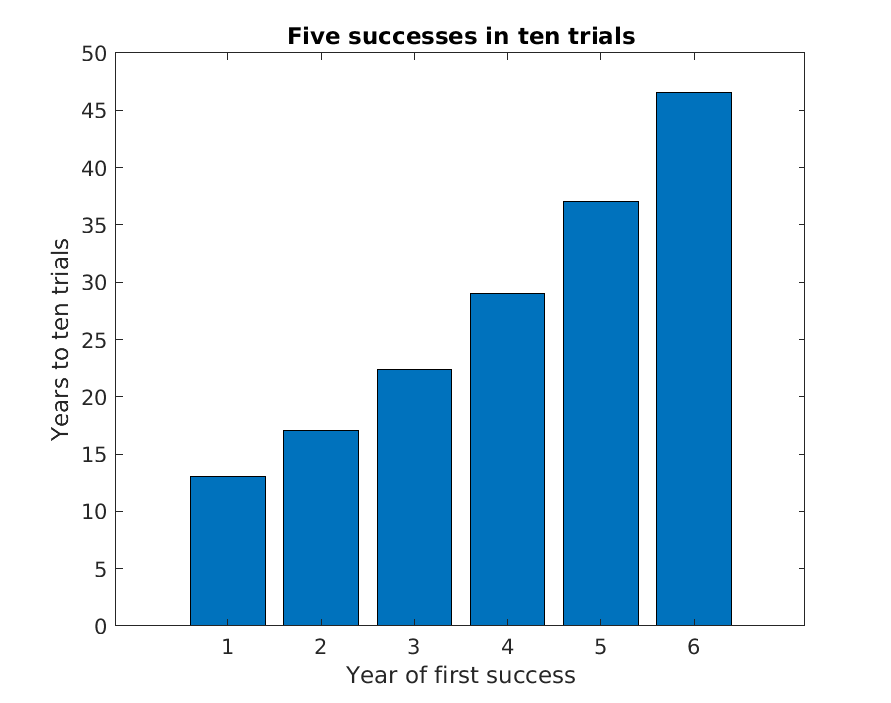
\includegraphics[width=\textwidth]{figures/success_order}
%        \caption{Baseline}
%    \end{subfigure}%
%    ~
%    \begin{subfigure}[b]{0.5\textwidth}
%        \centering
%        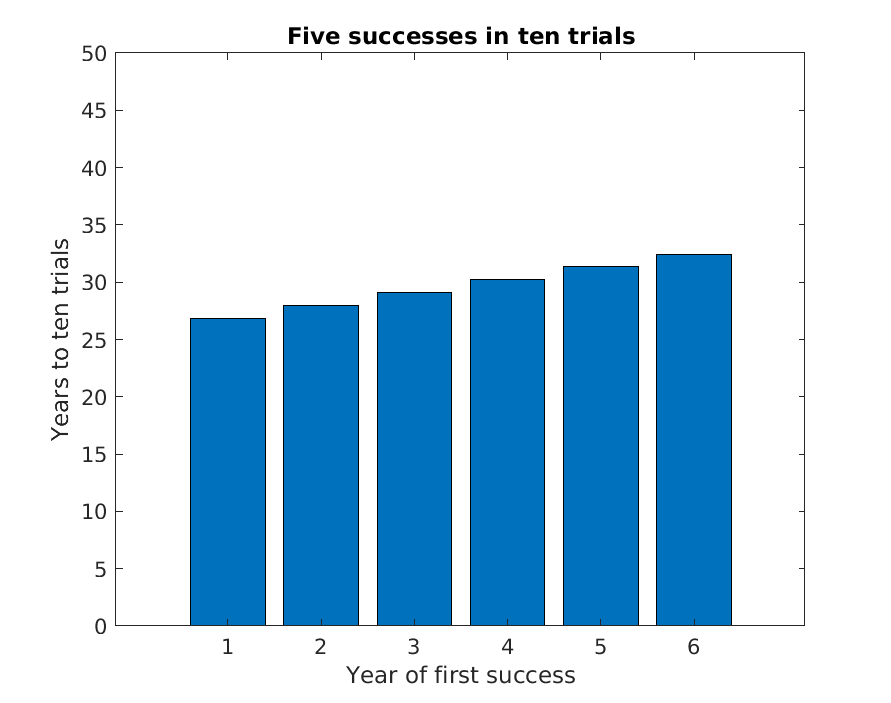
\includegraphics[width=\textwidth]{figures/success_order_nl}
%        \caption{No-learning}
%    \end{subfigure}
%    \caption{Time to ten meetings by placement of five consecutive successes}
%    \label{fig:success_order}
%\end{figure}

We can also examine how match arrival times depend on successes and failures
in the no-learning model. Since firms know their success probabilities in
this model, the no-learning version of Figure \ref{fig:success_beliefs} (not
pictured) is simply two horizontal lines with height $\theta ^{f}$. But the
lengths of these lines still depends upon match histories because of the
network effect. To demonstrate this dependence, Figure \ref%
{fig:success_order} plots the expected time to ten meetings, when five
consecutive meetings are successful and the others failures. The $x$-axis is
the number of meetings that take place before the first success occurs. If
it is one, then the first five meetings are successes, and the next five
failures. If it is 6, then the first five meetings are failures, and the
last five meetings successes.

To facilitate comparison, Figure \ref{fig:success_order} presents results
for both the baseline model (panel a) and the no learning model (panel b).
All plots are for a firm in the 90th percentile of productivity among
exporters, and, in the case of the no-learning model, the success
probability is set to $\theta ^{f}=0.43$. As we saw in Figure \ref%
{fig:success_beliefs}, the time it takes a learning firm to reach ten
meetings depends heavily on the placement of the successes (panel a). If the
successes come at the beginning of the ten meetings, it takes 12 years for
this type of firm to reach ten meetings. If the failures come first, it
takes 45 years. But for no-learning firms (panel b), time to ten meetings
depends much less on the placement of successes. If the successes come
first, it takes 27 years to reach ten meetings. If they come last, it takes
32 years.\footnote{%
The reason it takes so long is that this type of firm expects that only
around half of its meetings will be successes. This corresponds to the
ultimate 50\% success rate we are simulating, but it also means that the
firms are not searching very hard. If we were to make the firm believe that
it has a close to 100\% success rate, it would only take a few years to
reach 10 meetings.} So here again we see that learning effects and network
effects both matter, but the former are more important.

\subsection{Macroeconomic adjustment dynamics}

If there were no sources of friction in our model, and if the effects of
idioynscratic shocks were ignorable by the law of large numbers, aggregate
exports would be static functions of the aggegate shocks that affect all
firms' export revenues ($x^f$). We conclude our analysis by asking how much
our model's predictions for aggregate export trajectories deviate from this
hypothetical norm, and why.\footnote{%
Since we are using a single-agent model, we caution that these simulations
miss interactions between exporters in the foreign market. However, they may
be a reasonable approximation to the aggregate exports responses of a small
country shipping to a large one, where its products constitute a small
fraction of total supply.}

To do so, we simulate a permanent (but unanticipated) 20 percent Colombian
peso devaluation on total export trajectories under two alternative
scenarios: our benchmark model, and the no-learning model. For both
simulations, we use the same set of market-wide shocks. Specifically, we use
a series of randomly-generated aggregate rate shocks to simulate the model,
and then simulate the model again with the same shocks, but increasing their
values by 20\% after a particular date. The shock progression is graphed in
Figure \ref{fig:exch_shk_cmp}, with the shock arriving at time zero. As with
the rest of the series in this section, in the figure the shocks are
normalized to one at the time of impact.

% \begin{figure}
%    \centering
%    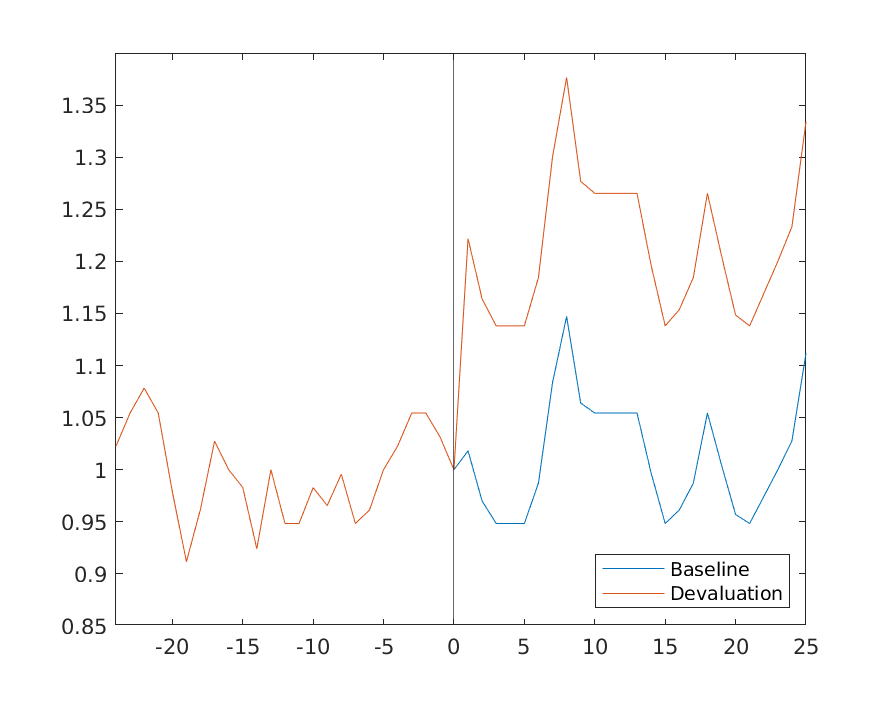
\includegraphics[scale = 0.5]{figures/exch_rate_series_compare}
%    \caption{Series of Peso to Dollar Exchange Rate Shocks, Baseline and with 20\% Peso Devaluation}
%    \label{fig:exch_shk_cmp}
%\end{figure}
%
%\begin{figure}
%    \centering
%    \begin{subfigure}[b]{0.5\textwidth}
%        \centering
%        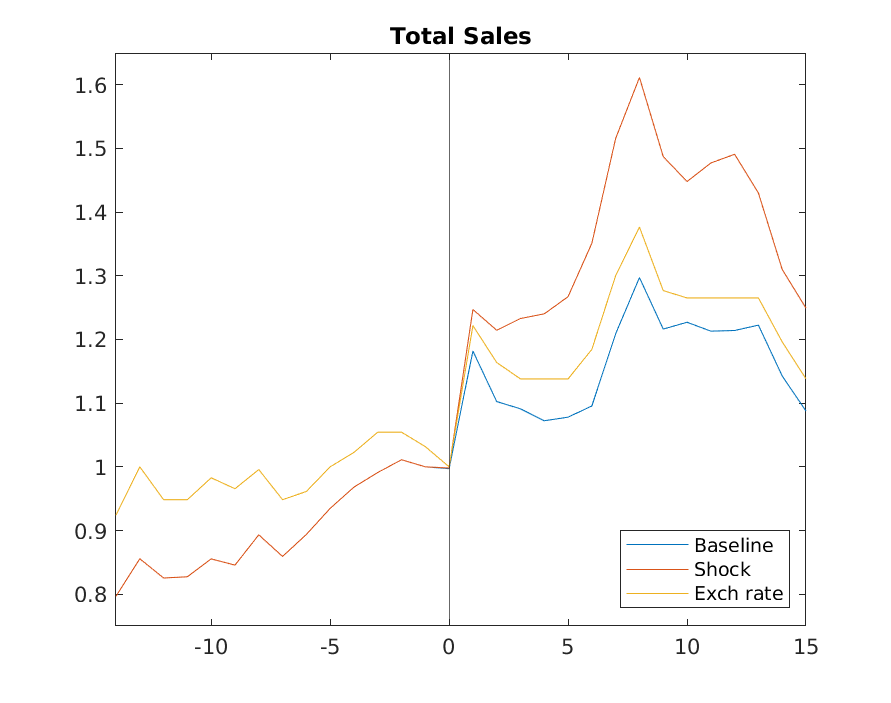
\includegraphics[width=\textwidth]{figures/total_sales}
%        \caption{Total sales}
%    \end{subfigure}%
%    ~
%    \begin{subfigure}[b]{0.5\textwidth}
%        \centering
%        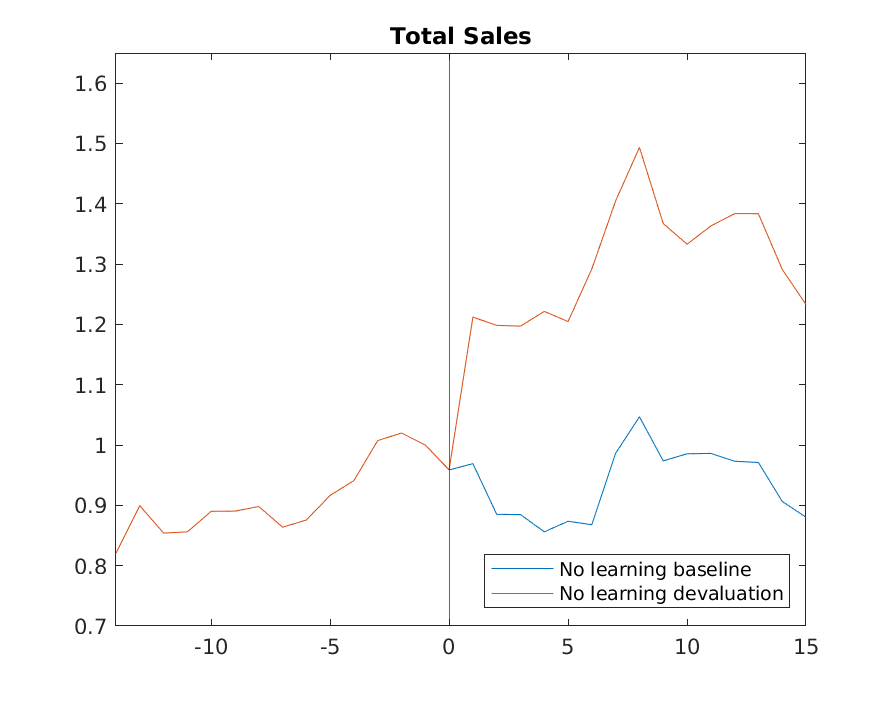
\includegraphics[width=\textwidth]{figures/total_sales_nl}
%        \caption{Total sales}
%    \end{subfigure} \\
%    ~
%    \begin{subfigure}[b]{0.5\textwidth}
%        \centering
%        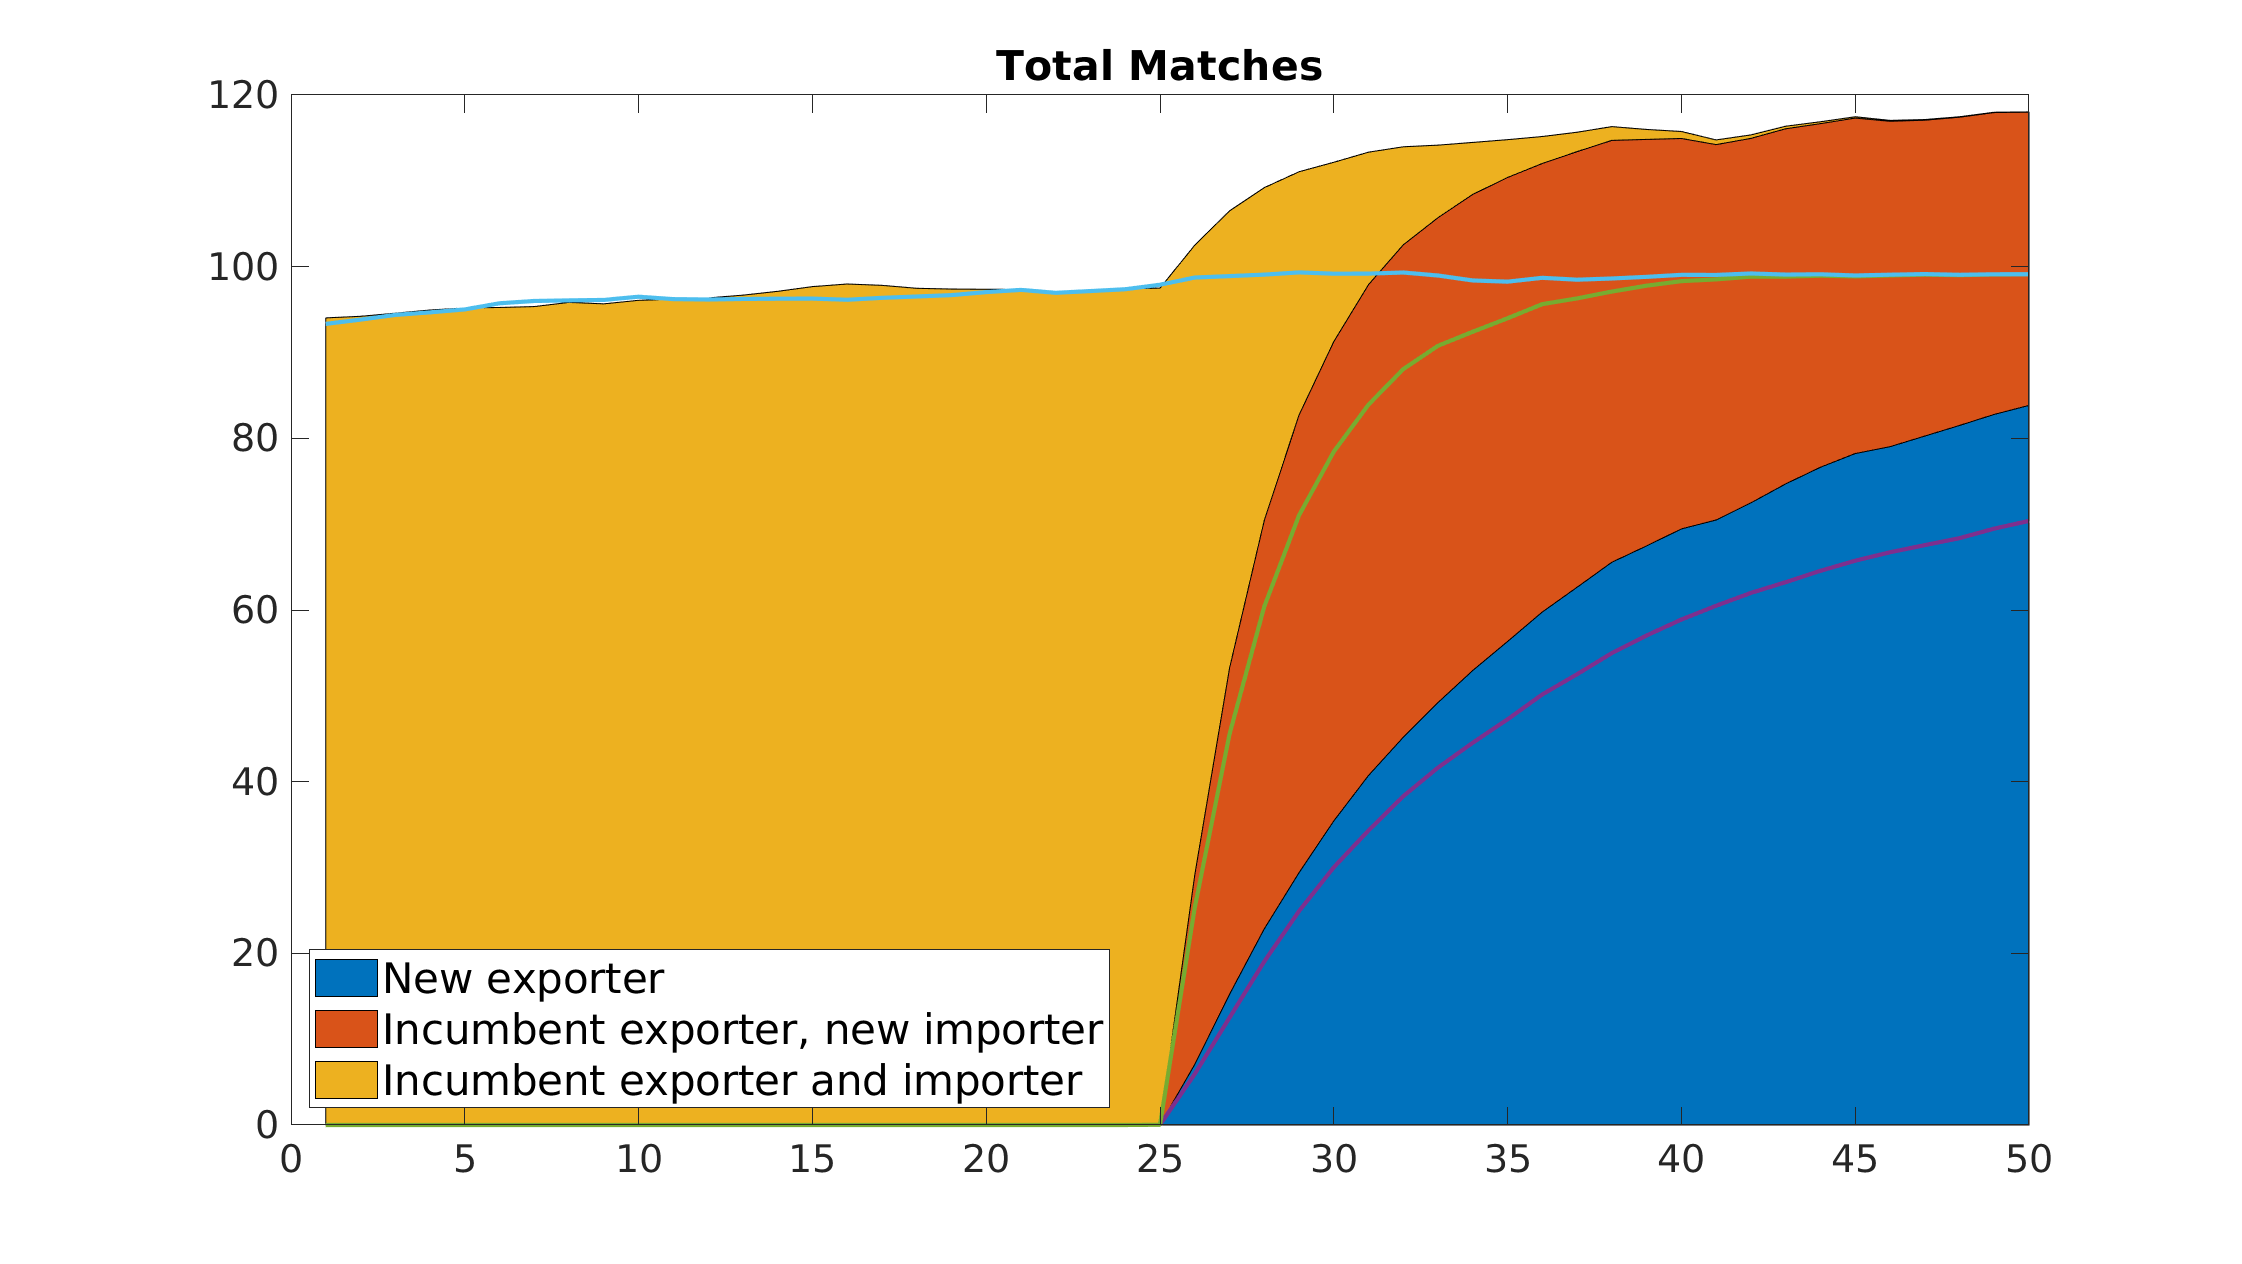
\includegraphics[width=\textwidth]{figures/total_matches}
%        \caption{Total active matches}
%    \end{subfigure}%
%    ~
%    \begin{subfigure}[b]{0.5\textwidth}
%        \centering
%        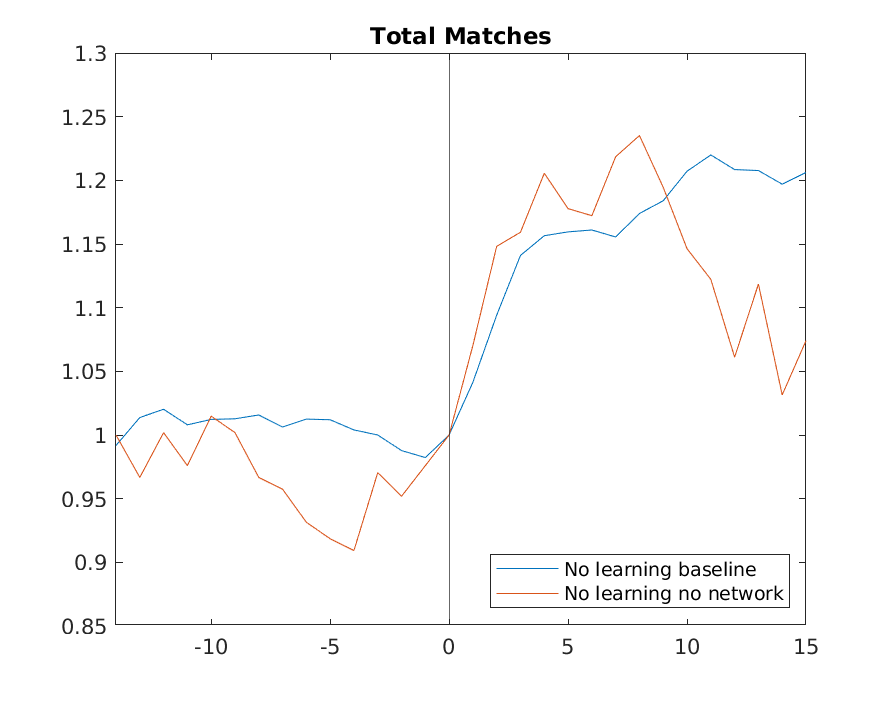
\includegraphics[width=\textwidth]{figures/total_matches_nl}
%        \caption{Total active matches}
%    \end{subfigure} \\
%    ~
%    \begin{subfigure}[b]{0.5\textwidth}
%        \centering
%        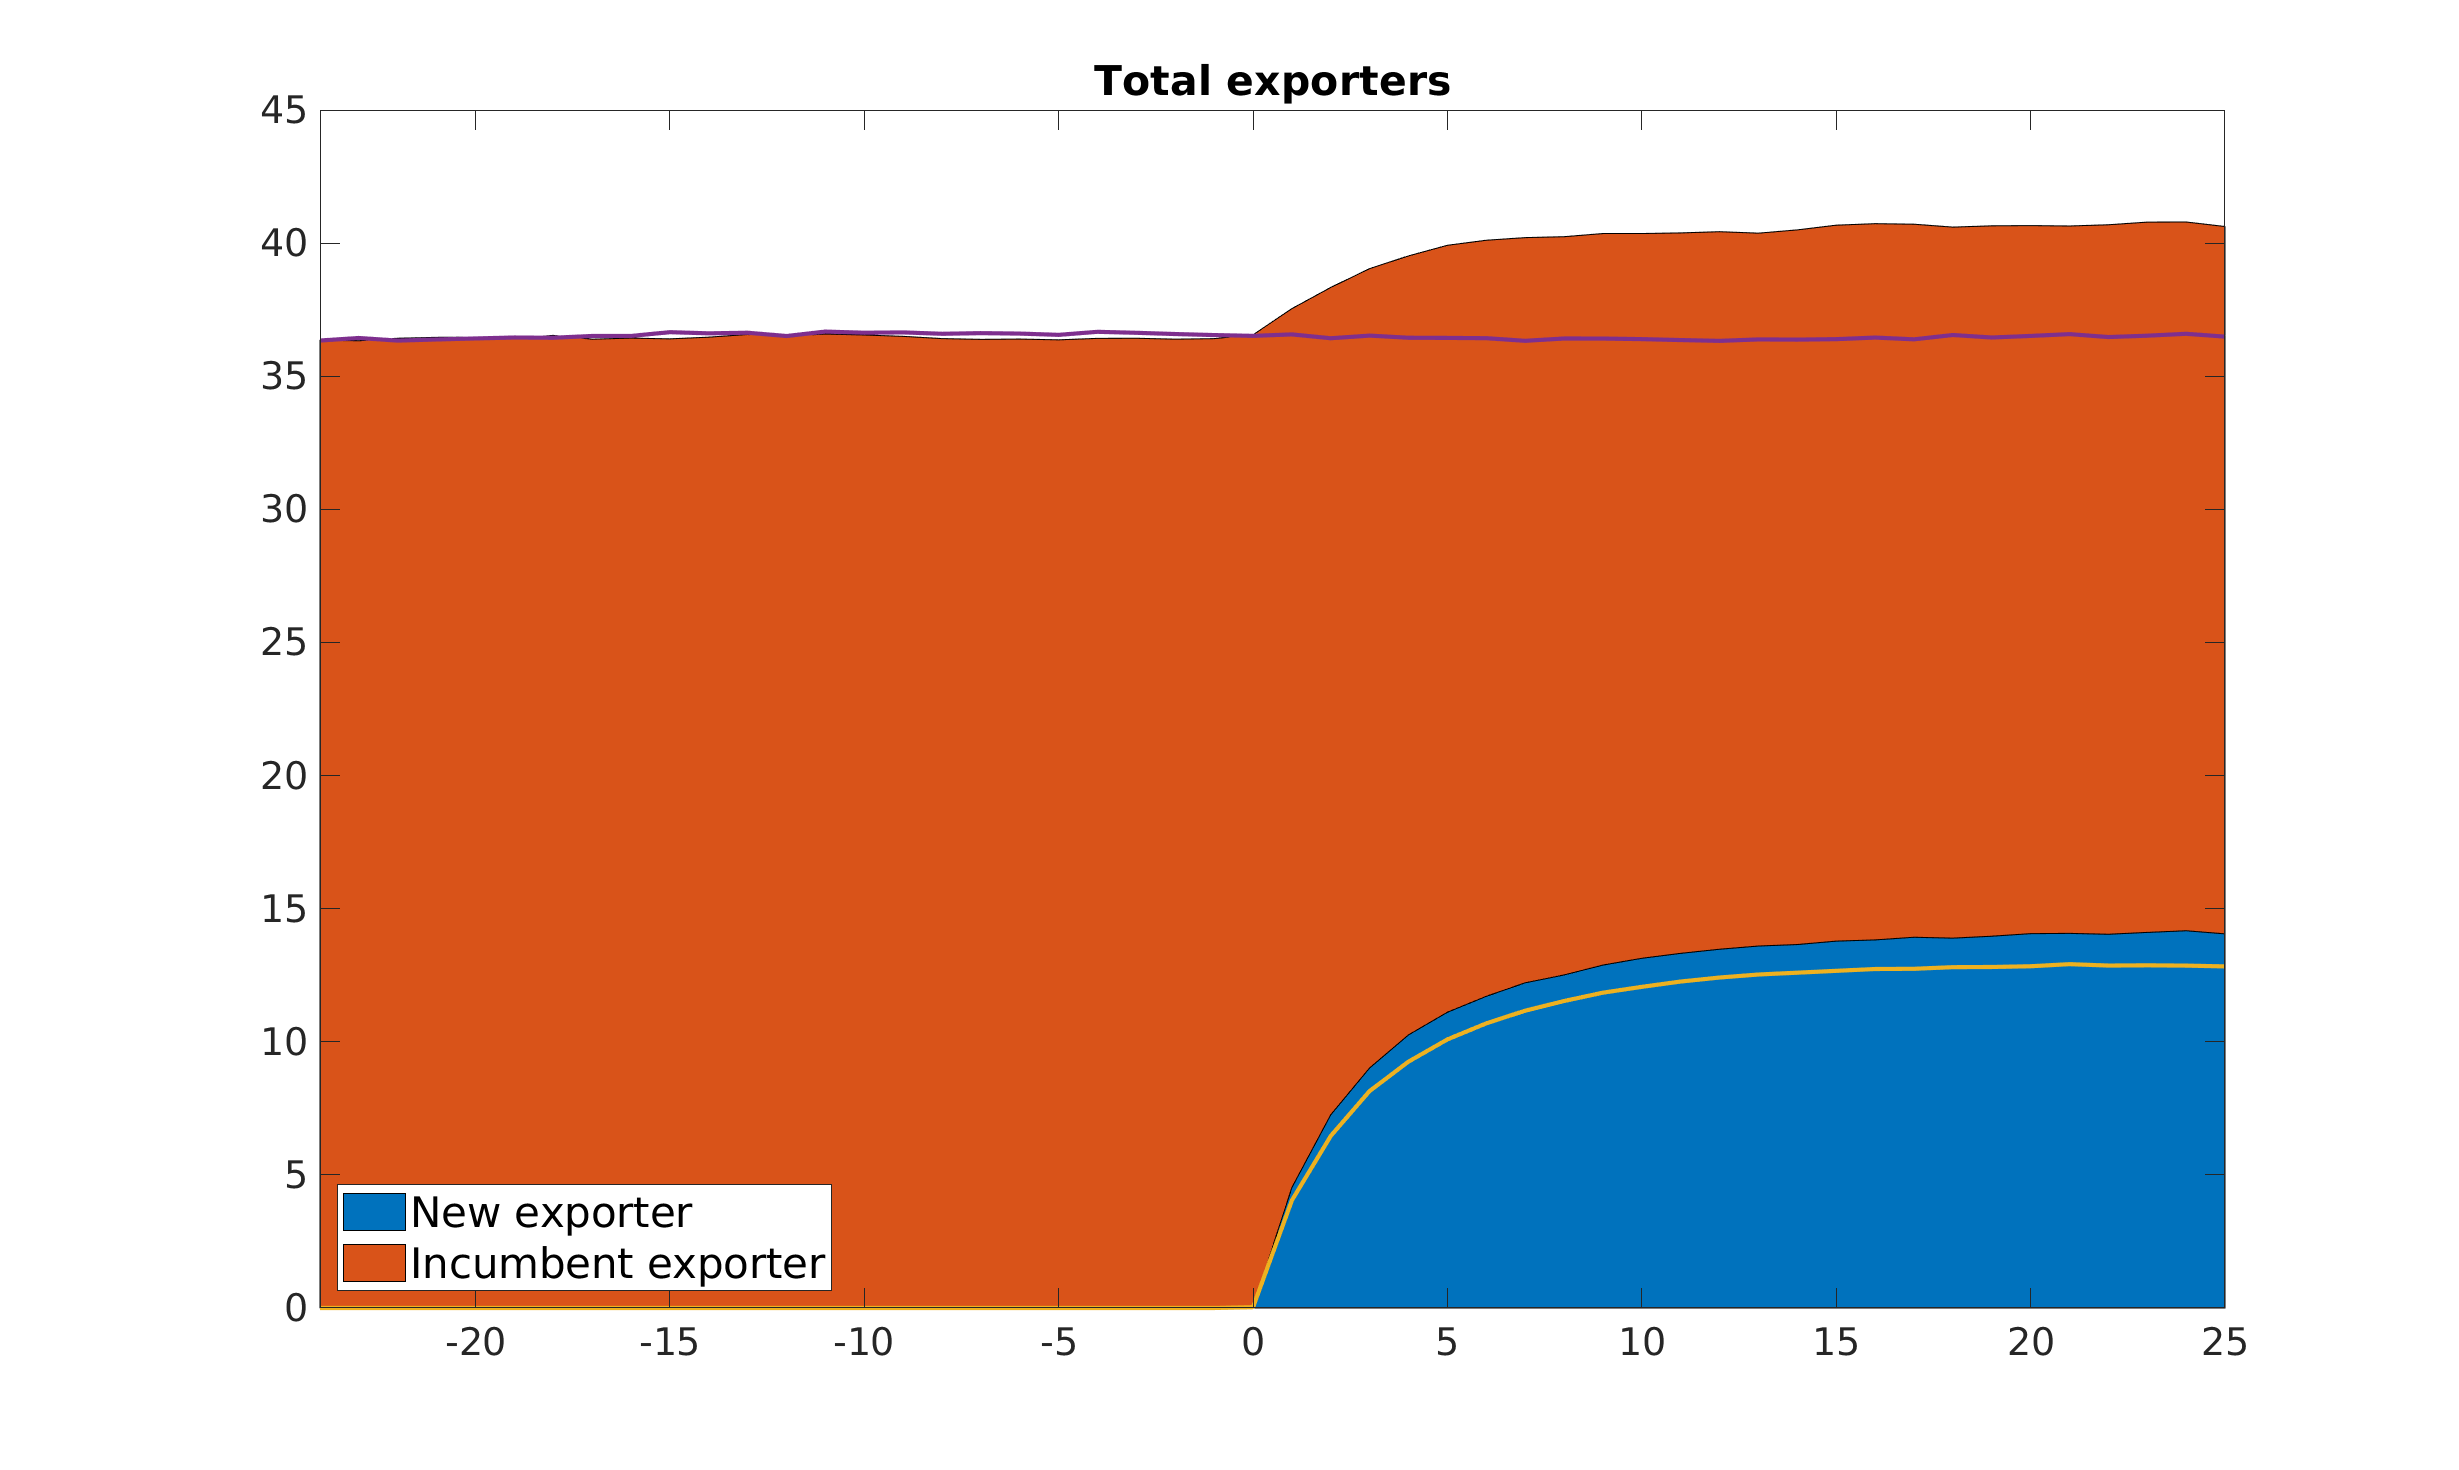
\includegraphics[width=\textwidth]{figures/total_firms}
%        \caption{Total active firms}
%    \end{subfigure}%
%    ~
%    \begin{subfigure}[b]{0.5\textwidth}
%        \centering
%        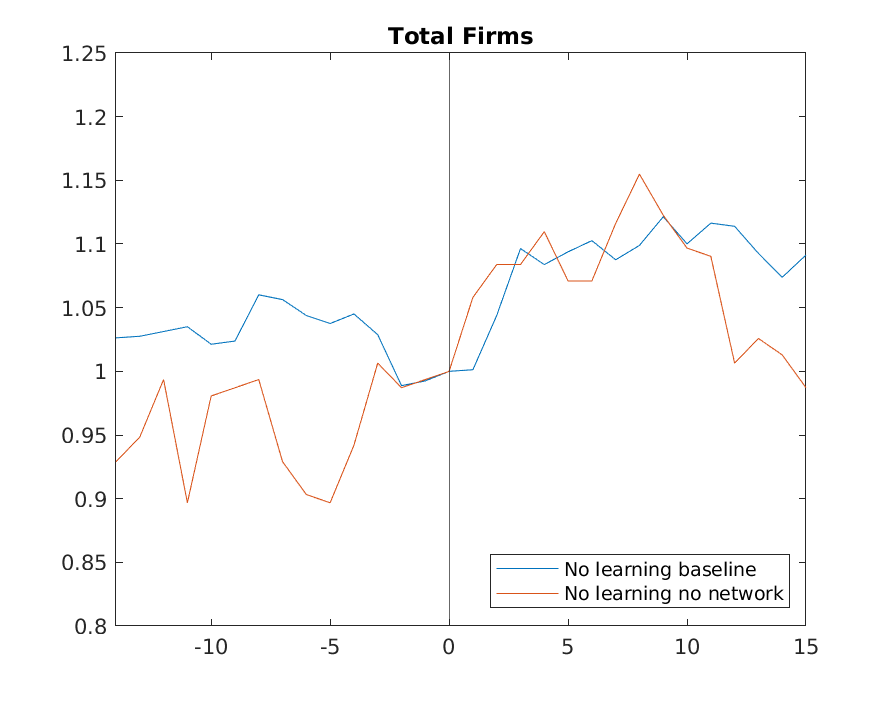
\includegraphics[width=\textwidth]{figures/total_firms_nl}
%        \caption{Total active firms}
%    \end{subfigure}
%    \caption{Response to a 20\% depreciation of Colombian Peso: Market level outcomes}
%    \label{fig:export_dynamics_macro}
%
%\end{figure}

% \begin{figure}
%     \centering
%     \begin{subfigure}[b]{0.5\textwidth}
%         \centering
%         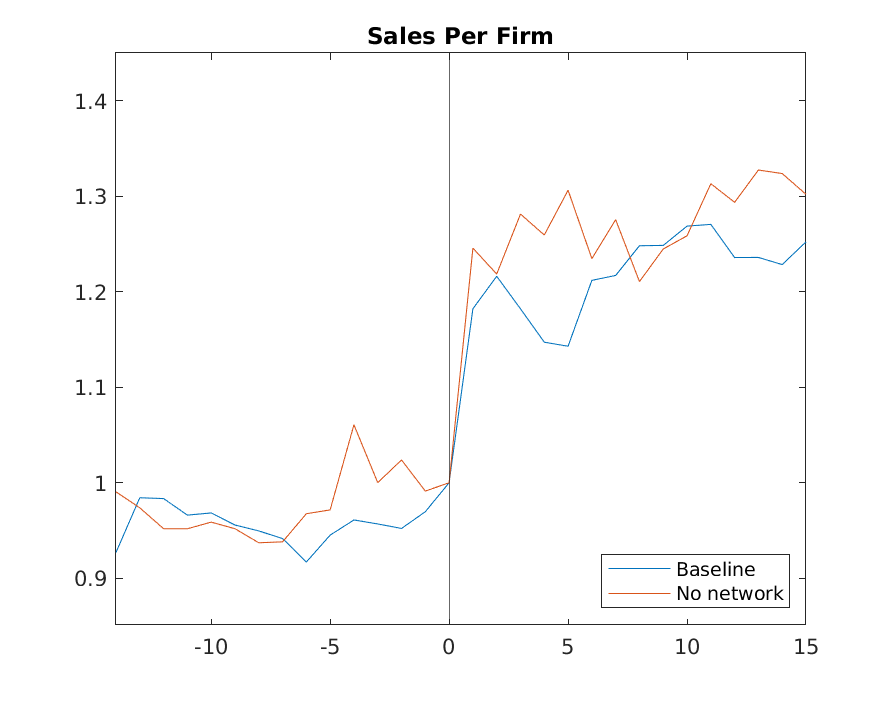
\includegraphics[width=\textwidth]{figures/sales_per_firm_l}
%         \caption{Sales per firm}
%     \end{subfigure}%
%     ~
%     \begin{subfigure}[b]{0.5\textwidth}
%         \centering
%         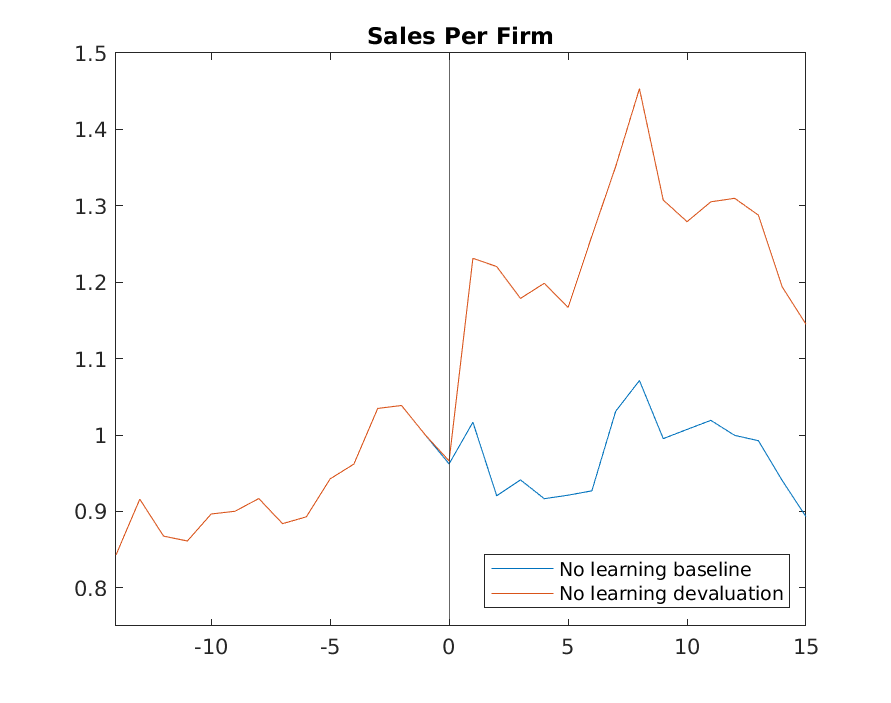
\includegraphics[width=\textwidth]{figures/sales_per_firm_nl}
%         \caption{Sales per firm}
%     \end{subfigure} \\
%     ~
%     \begin{subfigure}[b]{0.5\textwidth}
%         \centering
%         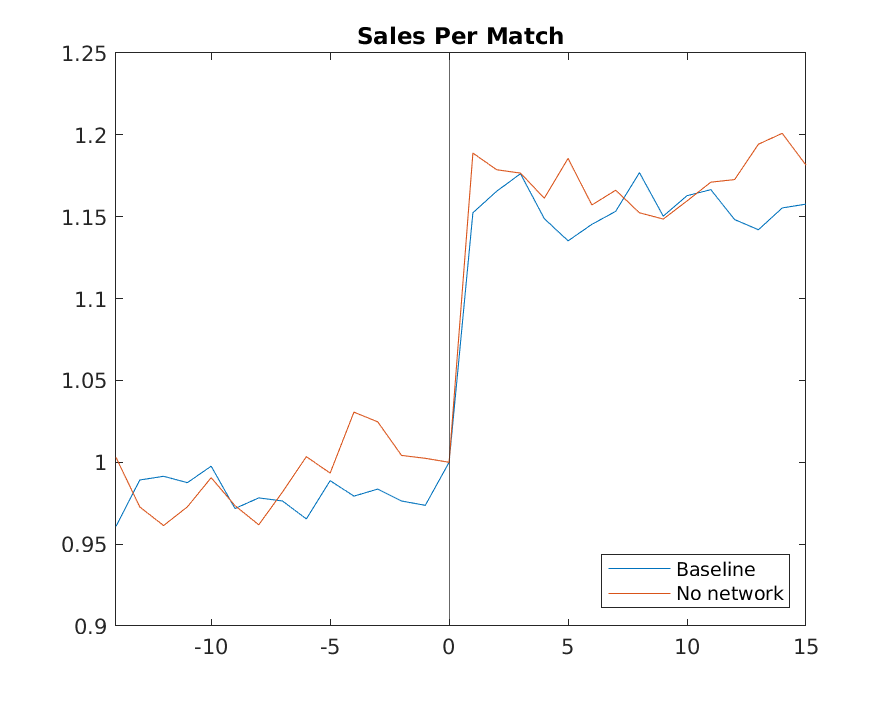
\includegraphics[width=\textwidth]{figures/sales_per_match_l}
%         \caption{Sales per match}
%     \end{subfigure}%
%     ~
%     \begin{subfigure}[b]{0.5\textwidth}
%         \centering
%         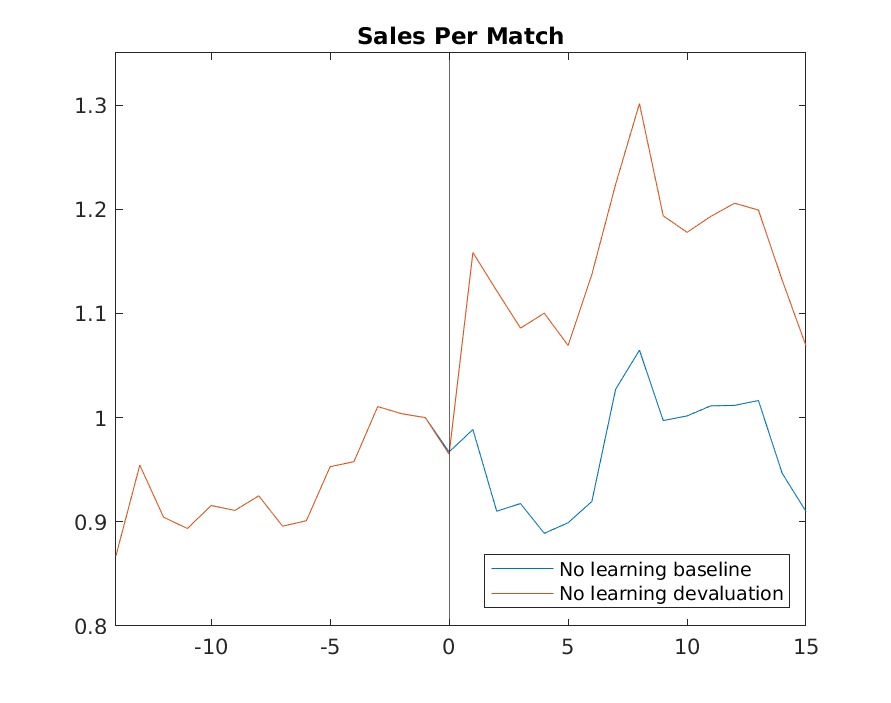
\includegraphics[width=\textwidth]{figures/sales_per_match_nl}
%         \caption{Sales per match}
%     \end{subfigure} \\
%     ~
%     \begin{subfigure}[b]{0.5\textwidth}
%         \centering
%         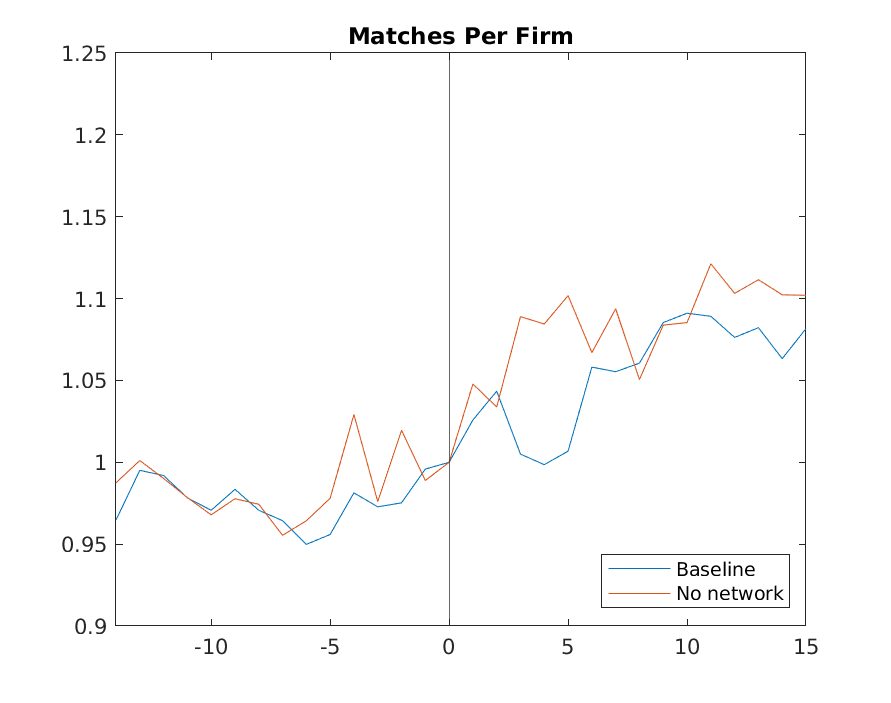
\includegraphics[width=\textwidth]{figures/matches_per_firm_l}
%         \caption{Matches per firm}
%     \end{subfigure}%
%     ~
%     \begin{subfigure}[b]{0.5\textwidth}
%         \centering
%         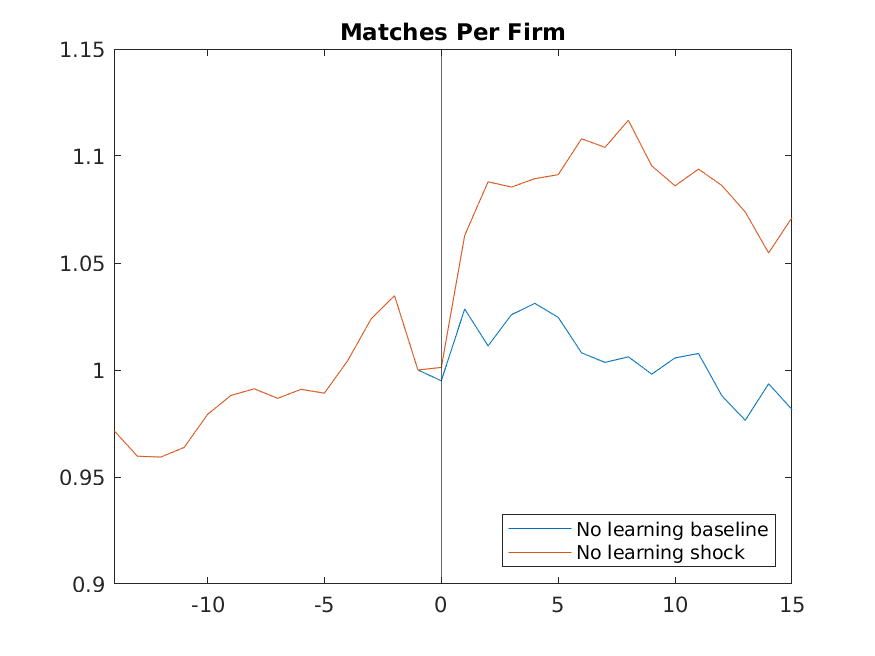
\includegraphics[width=\textwidth]{figures/matches_per_firm_nl}
%         \caption{Matches per firm}
%     \end{subfigure}
%     \caption{Response to a 20\% depreciation of Colombian Peso: Average outcomes}
%     \label{fig:export_dynamics_average}
% 
% \end{figure}

Figures \ref{fig:export_dynamics_macro} summarizes the results of these
experiments, normalizing each export series to unity in the year before the
shock hits (year -1). Consider Panel (a) and Panel (b) of Figure \ref%
{fig:export_dynamics_macro}, which plot total export sales over a 30 year
period bisected by the shock. In both versions of the model, the immediate
effect of the depreciation is to increase the peso-denominated revenue flow
from existing clients by 20 percent. And because other margins of adjustment
are sluggish, this valuation effect accounts for almost all of the movement
in aggregate exports during the first post-shock year.

The differences in these patterns trace largely to differences in the
numbers of matches, which are depicted in Panels (c) and (d) of Fgure \ref%
{fig:export_dynamics_macro}. Here the valuation effect plays no role, so it
is easier to see the difference between the baseline series and the two
series without learning. We interpret these patterns to mean that firms with
high success rates (large $\theta ^{f}$ values) jump into the export market
aggressively when they know their profit potential, but they go slow if they
do not, gaining confidence and intensifying their search efforts as positive
signals accrue.

What accounts for the high volatility of the no-learning, no-network series?
We have already noted that when firms know their type, the high-$\theta ^{f}$
exporters want to expand quickly when markets turn favorable. But if network
effects are missing, these same firms have relatively little incentive to
maintain a large client base when market conditions turn sour. Negative
aggregate shocks therefore trigger relatively rapid retrenchment when both
learning and network effects are absent.\textbf{\ [JT: Need to confirm that
aggregate worsen after year 8 or so.]}

In sum, learning effects and---to a lesser extent---network effects do
appear to lend persistence to aggregate bilateral export flows, adding
several years to the transition period in the aftermath of a permanent
shock. These results obtain because the relevant extensive margin here is
the match, not the firm. This means that adjustment on that margin matters
for dominant exporters and fringe players alike.

\pagebreak

\section{Summary}

\textbf{[JT: section not yet updated]} Customs records reveal tremendous
turnover among Colombian manufacturers who export to the U.S.. In a typical
year, 48 percent of these exporters are new to the U.S. market, and 81
percent of these new exporters will be gone two years hence. New exporters
ship small quantities, so despite their numbers they account for only 12
percent of total Colombian exports in value terms. But each new cohort of
Colombian exporters contains a small number of firms that survive and
rapidly expand, growing many times faster than aggregate Colombian exports.
They do so by adding U.S. clients to their customer base at a rapid rate.

After documenting these patterns, we develop a continuous time model that
explains them. Firms wishing to export must engage in costly search to
identify potential buyers abroad. The buyers they encounter either reject
their products or form finite-lived business relationships with them. Buyer
who form business relationships with exporters send them favorable signals
about the appeal of their products, and in doing so, encourage them to
search more intensively for additional buyers. Successful business
relationships also reduce search costs by improving sellers' visibility
(network effects). Finally, sellers' search intensities depend upon their
permanent idiosyncratic characteristics and marketwide conditions.

Fit using the method of simulated moments, the model replicates the patterns
in customs records described above and allows us quantify several types of
trade costs, including the search costs of identifying potential clients and
the costs of maintaining business relationships with existing clients. It
also allows us to estimate the network effect of previous exporting
successes on the costs of meeting new clients, and to characterize the
cumulative effects of learning on firms'search intensities. Both the
learning effect and the network effect prove to be quantitatively important.
Finally, our model provides a lens through which to view the seemingly
unpredictable responses of export flows to exchange rate fluctuations.

\begin{center}
\ \pagebreak

{\Large \textbf{References}}
\end{center}

\begin{description}
\item Aeberhardt, R., I. Buono, and H. Fadinger (2014): \textquotedblleft
Learning, incomplete contracts and export dynamics: theory and evidence from
French firms,\textquotedblright\ \textit{European Economic Review}, 68:
219--249

\item Albornoz, Facundo, Hector Calvo Pardo, Gregory Corcos, and Emanuel
Ornelas (2012) "Sequential Exporting," \textit{Journal of International
Economics} 88: 17-31.

\item Alessandria, George and Horag Choi (2007) "Do Sunk Costs of Exporting
Matter for Net Export Dynamics?" \textit{Quarterly Journal of Economics},
pp. 289-336.

\item Alessandria, George and Horag Choi (2014) "Establishment
heterogeneity, exporter dynamics, and the effects of trade liberalization." 
\textit{Journal of International Economics} 94: 207-233..

\item Alessandria, George, Sangeeta Pratap, and Vivian Yue (2014) "Export
Dynamics in Large Devaluations." Working Paper, Federal Reserve Bank of
Philadelphia.

\item Alessandria, George, Horag Choi, and Kim Ruhl (2018) "Trade Adjustment
Dynamics and the Welfare Gains from Trade." Working Paper, The University of
Rochester.

\item Araujo, Luis, Emanuel Ornelas and Giordano Mion (2016) "Institutions
and Export Dynamics" \textit{Journal of International Economics }98: 2-20.

\item Arkolakis, Konstantinos (2010) \textquotedblleft Market Access Costs
and the New Consumers Margin in International Trade,\textquotedblright\ 
\textit{Journal of Political Economy}, 118(6), pp. 1151-1199.

\item Arkolakis, Konstantinos (2015) \textquotedblleft A Unified Theory of
Firm Selection and Growth,\textquotedblright\ \textit{Quarterly Journal of
Economics} 131(1): 89-155.

\item Arkolakis, Konstantinos, Theodore Papageorgiou and Olga Timoshenko \
(2018). "Firm Learning and Growth,"\textit{\ Review of Economic Dynamics}
27: 146-168.

\item Atkeson, Andrew and Ariel Burstein (2010) "Innovation, Firm Dynamics,
and International Trade." \textit{Journal of Political Economy} 118(3):
433-484.

\item Berman, N., V. Rebeyrol, and V. Vicard (2019) "Demand learning and
Firm dynamics: Evidence from Exporters," \textit{Review of Economics and
Statistics }101(1): 91-106.

\item Bernard, Andrew, J. Bradford Jensen, J. Stephen J. Reading, and Peter
K. Schott (2007) \textquotedblleft Firms in International
Trade,\textquotedblright\ \textit{Journal of Economic Perspectives}. 21(3):
105-130.

\item Bernard, Andrew, Andreas Moxnes and Karen Helene Ulltveit-Moe. 2018.
"Two-Sided Heterogeneity and Trade." \textit{Review of Economics and
Statistics }100(3): 424-439.

\item Bernard, Andrew, and Andreas Moxnes (2018) "Networks and Trade." 
\textit{Annual Review of Economics} 10(65): 65-85.

\item Besedes, Tibor (2007). \textquotedblleft A Search Cost Perspective on
Formation and Duration of Trade,\textquotedblright\ Working Paper,
Department of Economics, Georgia Tech University.

\item Burstein, Ariel and Marc Melitz (2013) \textquotedblleft Trade
Liberalization and Firm Dynamics.\textquotedblright\ in \textit{Advances in
Economics and Econometrics Tenth World Congress}. Applied Economics,
Econometric Society Monographs. Vol. 2. Cambridge, UK: Cambridge University
Press.

\item Blum, Bernardo S., Sebastian Claro, and Ignatius Horstmann (2010).
\textquotedblleft Facts and Figures on Intermediated
Trade\textquotedblright\ \textit{American Economic Review, Papers and
Proceedings}. 100(2) 419-423.

\item Blum, Bernardo S., Sebastian Claro, and Ignatius Horstmann (2013).
"Occasional and Perennial Exports," \textit{Journal of International
Economics} 90(1), May 2013.

\item Brooks, Eileen (2006) \textquotedblleft Why don't firms export more?
Product Quality and Colombian Plants\textquotedblright\ \textit{Journal of
Development Economics,} 80: 160-178.

\item Chaney, Thomas (2014) \textquotedblleft The Network Structure of
International Trade,\textquotedblright\ \textit{American Economic Review}
104(11): 3600--3634

\item Das, Mita, Mark Roberts and James Tybout (2007) \textquotedblleft
Market Entry Costs, Producer Heterogeneity and Export
Dynamics,\textquotedblright\ \textit{Econometrica }75(3), pp. 837-874.

\item Dickstein, M. J. and E. Morales (2018): \textquotedblleft What do
exporters know?\textquotedblright\ \textit{Quarterly Journal of Economics}
133: 1753--1801.

\item Dom\'{\i}nguez, Juan Camilo, Jonathan Eaton, Marcela Eslava, and James
Tybout. (2010) "Search and Learning in Export Markets: Case Studies for
Colombia." Pennsylvania State University, Working Paper.

\item Drozd, Lukasz A. and Jaromir B. Nosal (2008) \textquotedblleft
Understanding International Prices: Customers as Capital,\textquotedblright\
Working Paper, The University of Wisconsin.

\item Eaton, Jonathan, Samuel Kortum, and Francis Kramarz (2011)
\textquotedblleft An Anatomy of International Trade: Evidence from French
Firms,\textquotedblright\ \textit{Econometrica} 79(5), pp. 1453-1498.

\item Eaton, Jonathan, Marcela Eslava, Maurice Kugler and James Tybout
(2008). \textquotedblleft Export Dynamics in Colombia: Firm-Level
Evidence,\textquotedblright\ in Elhanan Helpman, Dalia Marin and Thierry
Verdier, eds., T\textit{he Organization of Firms in a Global Economy},
Cambridge, MA: Harvard U. Press.

\item Eaton, Jonathan, Marcela Eslava, David Jinkins, C.J. Krizan, and James
Tybout (2014). \textquotedblleft A Search and Learning Model of Export
Dynamics,\textquotedblright\ working paper, Pennsylvania State U.

\item Eaton, Jonathan, David Jinkins, James Tybout, and Daniel Xu (2016)
"Two-sided Search in International Markets," working paper, Pennsylvania
State U.

\item Fitzgerald, Doireann, Stefanie Hallerz, and Yaniv Yedid-Levi (2019)
"How Exporters Grow." Working Paper, Federal Reserve Bank of Minneapolis.

\item Foster, Lucia, John Haltiwanger and Chad Syverson (2016) "The Slow
Growth of New Plants: Learning aboout Demand?" \textit{Economica} 83(329):
91-129.

\item Gouri\'{e}roux and Monfort, 1996. \textit{Simulation-Based Econometric
Methods}. New York: Oxford U. Press.

\item Impullitti, Giammario, Alfonso. Irarrazabal, and Luca Opromolla (2013)
"A Theory of Entry into and Exit From Export Markets," \textit{Journal of
International Economics} 90\textit{: }75-90.

\item Jovanovic, Boyan (1982) \textquotedblleft Selection and the Evolution
of Industry,\textquotedblright\ \textit{Econometrica,} 50: 649-670.

\item Li, Shengyu (2018) "A structural model of productivity, uncertain
demand, and export dynamics," \textit{Journal of International Economics}
115: 1-15.

\item Rocco Macchiavello and Ameet Morjaria 2015 "The Value of
Relationships: Evidence from a Supply Shock to Kenyan Rose Exports" \textit{%
American Economic Review}, 105(9): 2911-2945

\item Morales, Eduardo, Gloria Sheu, and Andres Zahler (2019) "Extended
Gravity." \textit{Review of Economic Studies} 86(6): 2668-2712

\item Melitz, Marc (2003) \textquotedblleft The Impact of Trade on
Intra-Industry Reallocations and Aggregate Industry
Productivity,\textquotedblright\ \textit{Econometrica }71, 1695-1725.

\item Nguyen, Daniel (2012) "Demand Uncertainty, Exporting Delays and
Exporting Failures,"\textit{\ Journal of International Economics }86:
336-344.

\item Piveteau, Paul (forthcoming) "An Empirical Dynamic Model of Trade with
Consumer Accumulation," \textit{American Economic Journal: Macroeconomics.}

\item Rauch, James and Joel Watson (2003) \textquotedblleft Starting Small
in an Unfamiliar Environment,\textquotedblright\ \textit{International
Journal of Industrial Organization} 21: 1021-1042.

\item Rivers, Douglas and Quang Vuong (2002). "Model Selection for Nonlinear
Dynamic Models," \textit{Econometrics Journal} 5: 1-19.

\item Ruhl, Kim (2008) "The International Elasticity Puzzle." Working Paper,
The University of Wisconsin.

\item Ruhl, Kim and Jonathan Willis (2017) \textquotedblleft New Exporter
Dynamics,\textquotedblright\ \textit{International Economic Review} 58(3):
703-725.

\item Shimer, Robert (2005) "The Cyclical Behavior of Equilibrium
Unemployment and Vacancies," \textit{The American Economic Review}, 95(1),
pp. 25-49.

\item Sugita, Yoichi, Kensuke Teshima, and Enrique Seira (2019) "Assortative
Matching of Exporters and Importers," Working paper, Hitotsubashi University.

\item Timoshenko, O. A. (2015): \textquotedblleft Learning versus sunk costs
explanations of export persistence,\textquotedblright\ \textit{European
Economic Review}, 79, 113--128\pagebreak
\end{description}

\appendix

\section{data tables}

\label{sec:data_tables}

\begin{sidewaystable}[bph]
\centering
{\footnotesize
    \begin{tabular}{l|rrrrrrrrrrrrrrrrrr|r} \hline \hline \\[1px]
year     & 1992  & 1993  & 1994  & 1995 & 1996 & 1997 & 1998 & 1999  & 2000  & 2001  & 2002  & 2003  & 2004  & 2005  & 2006  & 2007  & 2008  & 2009  & total \\ \hline \\[1px]
    1992 & 2,232 &       &       &      &      &      &      &       &       &       &       &       &       &       &       &       &       &       & 2,232 \\
1993     & 823   & 1,235 &       &      &      &      &      &       &       &       &       &       &       &       &       &       &       &       & 2,058 \\
1994     & 583   & 330   & 1,160 &      &      &      &      &       &       &       &       &       &       &       &       &       &       &       & 2,073 \\
1995     & 440   & 213   & 339   & 953  &      &      &      &       &       &       &       &       &       &       &       &       &       &       & 1,945 \\
1996     & 372   & 163   & 178   & 255  & 899  &      &      &       &       &       &       &       &       &       &       &       &       &       & 1,867 \\
1997     & 321   & 128   & 133   & 170  & 248  & 877  &      &       &       &       &       &       &       &       &       &       &       &       & 1,877 \\
1998     & 268   & 104   & 124   & 132  & 153  & 256  & 893  &       &       &       &       &       &       &       &       &       &       &       & 1,930 \\
1999     & 232   & 85    & 87    & 114  & 117  & 187  & 262  & 1,026 &       &       &       &       &       &       &       &       &       &       & 2,110 \\
2000     & 203   & 85    & 79    & 91   & 103  & 136  & 170  & 344   & 1,372 &       &       &       &       &       &       &       &       &       & 2,583 \\
2001     & 187   & 70    & 65    & 79   & 85   & 109  & 145  & 229   & 389   & 1,251 &       &       &       &       &       &       &       &       & 2,609 \\
2002     & 173   & 64    & 62    & 72   & 68   & 88   & 112  & 171   & 242   & 399   & 1,373 &       &       &       &       &       &       &       & 2,824 \\
2003     & 165   & 51    & 58    & 62   & 62   & 77   & 86   & 140   & 185   & 301   & 440   & 1,719 &       &       &       &       &       &       & 3,346 \\
2004     & 150   & 52    & 41    & 53   & 63   & 76   & 80   & 132   & 164   & 223   & 327   & 616   & 1,768 &       &       &       &       &       & 3,745 \\
2005     & 140   & 52    & 47    & 39   & 54   & 77   & 69   & 115   & 145   & 196   & 235   & 398   & 661   & 1,902 &       &       &       &       & 4,130 \\
2006     & 122   & 46    & 44    & 39   & 44   & 71   & 65   & 110   & 131   & 157   & 168   & 308   & 410   & 564   & 1,896 &       &       &       & 4,175 \\
2007     & 113   & 37    & 39    & 31   & 42   & 55   & 48   & 91    & 101   & 132   & 156   & 240   & 305   & 365   & 548   & 1,681 &       &       & 3,984 \\
2008     & 93    & 29    & 30    & 24   & 38   & 50   & 45   & 74    & 90    & 117   & 130   & 184   & 198   & 230   & 331   & 447   & 1,455 &       & 3,565 \\
2009     & 80    & 25    & 28    & 24   & 28   & 40   & 39   & 60    & 72    & 88    & 97    & 145   & 175   & 157   & 230   & 248   & 386   & 1,378 & 3,300 \\ \hline

    \end{tabular}
}
    \caption{\textbf{Number of Exporting Firms, by Entry Cohort}}
    \label{tab:firm_num_by_cohort}\centering
\end{sidewaystable}

\begin{sidewaystable}[bph]
    \centering 
    {\footnotesize
    \begin{tabular}{l|rrrrrrrrrrrrrrrrrr|r} \hline \hline \\[1px]
year & 1992 & 1993 & 1994 & 1995 & 1996 & 1997 & 1998 & 1999 & 2000 & 2001 & 2002 & 2003 & 2004 & 2005 & 2006 & 2007 & 2008 & 2009 & total \\ \hline \\[1px]
1992 & 469  &      &      &      &      &      &      &      &      &      &      &      &      &      &      &      &      &      & 469 \\
1993 & 352  & 83   &      &      &      &      &      &      &      &      &      &      &      &      &      &      &      &      & 435 \\
1994 & 336  & 83   & 92   &      &      &      &      &      &      &      &      &      &      &      &      &      &      &      & 510 \\
1995 & 313  & 75   & 102  & 58   &      &      &      &      &      &      &      &      &      &      &      &      &      &      & 549 \\
1996 & 256  & 67   & 62   & 40   & 60   &      &      &      &      &      &      &      &      &      &      &      &      &      & 484 \\
1997 & 247  & 84   & 43   & 41   & 48   & 119  &      &      &      &      &      &      &      &      &      &      &      &      & 581 \\
1998 & 225  & 49   & 42   & 36   & 45   & 131  & 63   &      &      &      &      &      &      &      &      &      &      &      & 590 \\
1999 & 207  & 51   & 49   & 41   & 39   & 197  & 74   & 81   &      &      &      &      &      &      &      &      &      &      & 739 \\
2000 & 180  & 53   & 55   & 37   & 51   & 102  & 53   & 158  & 109  &      &      &      &      &      &      &      &      &      & 799 \\
2001 & 150  & 22   & 51   & 41   & 28   & 57   & 36   & 80   & 101  & 111  &      &      &      &      &      &      &      &      & 677 \\
2002 & 124  & 23   & 47   & 34   & 27   & 28   & 23   & 45   & 65   & 83   & 40   &      &      &      &      &      &      &      & 538 \\
2003 & 147  & 42   & 51   & 31   & 42   & 24   & 22   & 37   & 71   & 107  & 50   & 78   &      &      &      &      &      &      & 702 \\
2004 & 156  & 43   & 53   & 19   & 57   & 21   & 23   & 42   & 78   & 106  & 60   & 107  & 90   &      &      &      &      &      & 855 \\
2005 & 150  & 22   & 75   & 17   & 52   & 18   & 23   & 43   & 78   & 80   & 58   & 81   & 75   & 84   &      &      &      &      & 855 \\
2006 & 117  & 31   & 52   & 14   & 64   & 43   & 17   & 38   & 61   & 79   & 32   & 51   & 52   & 112  & 78   &      &      &      & 838 \\
2007 & 103  & 7    & 18   & 11   & 67   & 58   & 19   & 30   & 28   & 64   & 22   & 35   & 33   & 66   & 67   & 62   &      &      & 689 \\
2008 & 95   & 6    & 9    & 8    & 33   & 37   & 17   & 33   & 26   & 34   & 20   & 31   & 37   & 54   & 42   & 53   & 57   &      & 591 \\
2009 & 68   & 22   & 7    & 6    & 13   & 24   & 10   & 23   & 16   & 16   & 14   & 22   & 41   & 25   & 39   & 37   & 36   & 64   & 485 \\ \hline
    \end{tabular} 
    }
    \caption{\textbf{Value of Exports, by Entry Cohort (millions of \$US)}}
    \label{tab:exp_val_by_cohort}\centering
\end{sidewaystable}

\begin{sidewaystable}[bph]
    \centering
    {\footnotesize
    \begin{tabular}{l|rrrrrrrrrrrrrrrrrrrr|r} \hline \hline \\[1px]
year & 1992  & 1993 & 1994  & 1995 & 1996  & 1997  & 1998 & 1999 & 2000 & 2001 & 2002 & 2003 & 2004 & 2005 & 2006 & 2007 & 2008 & 2009 & pooled \\ \hline \\[1px]
1992 & 210   &      &       &      &       &       &      &      &      &      &      &      &      &      &      &      &      &      & 210 \\
1993 & 428   & 67   &       &      &       &       &      &      &      &      &      &      &      &      &      &      &      &      & 211 \\
1994 & 576   & 251  & 79    &      &       &       &      &      &      &      &      &      &      &      &      &      &      &      & 246 \\
1995 & 712   & 353  & 300   & 61   &       &       &      &      &      &      &      &      &      &      &      &      &      &      & 282 \\
1996 & 687   & 411  & 346   & 158  & 67    &       &      &      &      &      &      &      &      &      &      &      &      &      & 259 \\
1997 & 771   & 652  & 321   & 241  & 192   & 136   &      &      &      &      &      &      &      &      &      &      &      &      & 310 \\
1998 & 839   & 468  & 339   & 269  & 297   & 510   & 71   &      &      &      &      &      &      &      &      &      &      &      & 306 \\
1999 & 893   & 601  & 561   & 361  & 336   & 1,054 & 281  & 79   &      &      &      &      &      &      &      &      &      &      & 350 \\
2000 & 885   & 623  & 697   & 407  & 496   & 750   & 313  & 460  & 80   &      &      &      &      &      &      &      &      &      & 309 \\
2001 & 801   & 316  & 783   & 519  & 329   & 521   & 251  & 350  & 259  & 89   &      &      &      &      &      &      &      &      & 260 \\
2002 & 716   & 353  & 757   & 473  & 399   & 318   & 207  & 260  & 268  & 207  & 29   &      &      &      &      &      &      &      & 191 \\
2003 & 891   & 827  & 870   & 493  & 677   & 315   & 257  & 260  & 385  & 355  & 114  & 46   &      &      &      &      &      &      & 210 \\
2004 & 1,039 & 828  & 1,281 & 358  & 900   & 281   & 291  & 318  & 478  & 476  & 183  & 174  & 51   &      &      &      &      &      & 228 \\
2005 & 1,071 & 413  & 1,593 & 444  & 967   & 231   & 326  & 375  & 535  & 408  & 248  & 204  & 113  & 44   &      &      &      &      & 207 \\
2006 & 958   & 675  & 1,177 & 356  & 1,448 & 605   & 256  & 341  & 464  & 505  & 188  & 165  & 126  & 198  & 41   &      &      &      & 201 \\
2007 & 915   & 175  & 466   & 357  & 1,606 & 1,048 & 391  & 327  & 278  & 481  & 140  & 145  & 108  & 181  & 123  & 37   &      &      & 173 \\
2008 & 1,023 & 208  & 283   & 341  & 860   & 747   & 379  & 443  & 289  & 287  & 153  & 166  & 186  & 236  & 125  & 120  & 39   &      & 166 \\
2009 & 855   & 864  & 262   & 266  & 478   & 607   & 255  & 389  & 221  & 176  & 143  & 152  & 235  & 162  & 169  & 151  & 93   & 47   & 147 \\ \hline
    \end{tabular}
    }
    \caption{\textbf{Exports per Firm, by Entry Cohort (thousands of \$US)}}
    \label{tab:exp_per_firm_by_cohort}\centering
\end{sidewaystable}

\begin{table}[bph]
\centering
\begin{tabular}{lrrr}
\hline\hline
&  &  &  \\[1px] 
Year & Colombian Sellers & U.S. Importers & Pairs \\ \hline
&  &  &  \\[1px] 
1992 & 2,232 & 1,190 & 3,087 \\ 
1993 & 2,058 & 1,183 & 2,824 \\ 
1994 & 2,073 & 1,212 & 2,810 \\ 
1995 & 1,945 & 1,173 & 2,588 \\ 
1996 & 1,867 & 1,191 & 2,490 \\ 
1997 & 1,877 & 1,208 & 2,480 \\ 
1998 & 1,930 & 1,191 & 2,495 \\ 
1999 & 2,110 & 1,386 & 2,793 \\ 
2000 & 2,583 & 1,661 & 3,411 \\ 
2001 & 2,609 & 1,698 & 3,483 \\ 
2002 & 2,824 & 1,826 & 3,733 \\ 
2003 & 3,346 & 2,110 & 4,483 \\ 
2004 & 3,745 & 2,296 & 5,071 \\ 
2005 & 4,130 & 2,457 & 5,552 \\ 
2006 & 4,175 & 2,471 & 5,607 \\ 
2007 & 3,984 & 2,343 & 5,307 \\ 
2008 & 3,565 & 2,221 & 4,751 \\ 
2009 & 3,300 & 2,079 & 4,467 \\ \hline
\end{tabular}
\centering{\small \ }
\caption{\textbf{Exporters and importers by year}}
\label{tab:ex_im_by_year}
\end{table}

\pagebreak

\section{Data checks}

\label{sec:data_check}

To investigate the quality of the exporter id (manuf\_id) in the U.S. import
records, we ran a series of robustness checks. The Colombian and U.S. data
overlap for the years 2000-2008 and both contain measures of the value of
exports as well as the number of exporting firms. If the manuf\_id variable
is error-prone and noisy, we would expect the U.S. data to over-report the
number of Colombian firms exporting to the U.S. That is, each time a customs
broker wrongly enters the data in the field, a new firm would be created.
Table \ref{tab:ap_dat_comp} below summarizes the total value of exports to
the U.S. and the number of Colombian firms, by year, for each data set.

\begin{table}[tbp]
\centering
{\small 
\begin{tabular}{l}
\begin{tabular}{rrrrlrr}
\hline\hline
& \multicolumn{2}{r}{\textbf{Colombia}} & \multicolumn{2}{r}{\textbf{United
States}} & \multicolumn{2}{r}{\textbf{\% difference}} \\ \cline{2-7}
Year & \# exporters & value & \# exporters & value & \# exporters & value \\ 
\hline
2000 & 1775 & 1038 & 2721 & 1140 & 53\% & 10\% \\ 
2001 & 2026 & 995 & 2744 & 1019 & 35\% & 2\% \\ 
2002 & 2230 & 870 & 2986 & 855 & 34\% & -2\% \\ 
2003 & 2800 & 1113 & 3579 & 1119 & 28\% & 1\% \\ 
2004 & 3035 & 1379 & 4002 & 1415 & 32\% & 3\% \\ 
2005 & 2861 & 1554 & 4288 & 1438 & 50\% & -7\% \\ 
2006 & 2689 & 1665 & 4361 & 1552 & 62\% & -7\% \\ 
2007 & 2420 & 1540 & 4175 & 1496 & 73\% & -3\% \\ 
2008 & 2161 & 1570 & 3758 & 1474 & 74\% & -6\% \\ \hline
\end{tabular}%
\end{tabular}%
}
\caption{\textbf{Colombian versus U.S. Customs Records}}
\label{tab:ap_dat_comp}
\end{table}

The datasets align much more closely on value than they do on firm counts.
The difference in value is never more than 10\% while the firm count
difference ranges from 18\% to 74\%. The differences are stable over time.

To look more closely at the cause of the difference in firm counts, we
compared the number of firms across sources by HS2 categories. The counts in
the LFTTD were higher than the Colombian data in only 28 of the 82 codes and
by far the biggest differences are in HS codes 61 and 62: textiles. In these
two product classes the U.S. data identifies 4025 more firms than the
Colombian data. If we remove these two sectors from the list, the difference
in firm counts flips and the Colombian data contain 1001 more firms than the
LFTTD.

Interestingly, Title 19 of U.S. code specifically requires that the
manuf\_id variable for textile products represent the manufacturer of the
textile products, not an intermediary. That is, for this sector in
particular the manufacturer, not an intermediary must be reported on the CBP
7501 form. By contrast, prior work by several authors of this paper has
shown (Marcela's 8/9/13 e-mail referenced this) that the Colombian data
reports the exporter, which may or may not be the manufacturer. Given that
revious research (Tybout, 2000 JEL) has shown that developing countries tend
to have a disproportionately large share of small manufacturing firms, it is
reasonable to assume that a large part of the reason why the U.S. data
report so many more firms in the textile sector is that due to
administrative reasons the U.S. data count many small manufacturers and the
Colombian data are, in many cases, reporting aggregators and intermediaries.

As a final check of the integrity of the manuf\_id variable - and the
robustness of our main results - we experimented with a \textquotedblleft
fuzzy\textquotedblright\ version of the manuf\_id variable that did not
contain any street numbers in the string (a likely source of input errors).
The effect of this is to reduce the number of Colombian firms in the data,
an approximation of fixing any extraneous noise from data entry errors. Next
we re-ran Table \ref{tab:sep_rates} with the fuzzy data and compared the
results to the original version.

One of the key findings from Table \ref{tab:sep_rates} is the high match
separation rates ranging from about 40\% to 66\%. Using the fuzzy version
did not reduce the separation rates substantially and left the patterns
intact. The fuzzy separation rates ranged from 26\% to 62\%, a drop of 6\%
on average. It does not appear that our results are sensitive to a modest
reduction in data entry errors.\newline
\pagebreak \bigskip

\section{Identification}

\label{sec:sensitivity}

\begin{table}[tbp]
\caption{\textbf{Sensitivity matrix} }%
\resizebox{\textwidth}{!}{
\bigskip

\begin{tabular}{rrrrrrrrrrrrr}
& $\ln {\small \Pi }^{h}$ & $F^{h}$ & $F^{f}$ & $\ln {\small \Pi }^{f}$ & ${\small \alpha }$ & ${\small \beta }$ & $\Delta _{y}$ & ${\small \lambda }_{b}$ & ${\small \gamma }$ & $\ln {\small \kappa _{0}^{h}}$ & $\ln {\small \kappa _{0}^{f}}$ & $\sigma _{\varphi }$ \\ 
\textbf{avg. mat death} & -0.112 & 0.007 & 0.011 & -0.111 & -0.019 & 0.127 & 
0.006 & 0.068 & -0.045 & -0.097 & -0.119 & 0.000 \\ 
new to mkt & -0.841 & -0.034 & 0.420 & -0.656 & -0.283 & 0.772 & 1.199 & 
-0.325 & -0.482 & 0.329 & 0.131 & 0.040 \\ 
current sales & -2.164 & 0.294 & 2.080 & 2.905 & 0.003 & 0.454 & 11.016 & 
4.386 & -2.072 & -12.437 & -3.520 & -0.326 \\ 
exporter age & 1.027 & 0.092 & -0.745 & 1.029 & 0.411 & -1.124 & -1.216 & 
1.074 & 0.586 & -0.966 & -0.726 & -0.089 \\ 
match age & -0.876 & 0.117 & -0.216 & -0.557 & 0.068 & 0.868 & -0.389 & 1.422
& -0.136 & -2.108 & -1.579 & -0.045 \\ 
\textbf{avg. match sales} & 0.190 & -0.012 & -0.042 & 0.075 & 0.040 & -0.045
& -0.228 & -0.176 & 0.072 & 0.256 & 0.214 & 0.011 \\ 
1st yr dummy & 1.616 & -0.096 & 0.462 & 5.391 & 0.419 & -4.141 & 6.635 & 
1.058 & 0.501 & -2.377 & 2.464 & -0.175 \\ 
match sales, t-1 & -0.683 & 0.058 & -0.097 & -1.127 & -0.183 & 1.293 & 0.170
& 0.742 & -0.469 & -0.082 & -1.077 & 0.012 \\ 
exporter age & 0.428 & -0.047 & 0.196 & 1.050 & 0.169 & -1.178 & -0.081 & 
-0.493 & 0.410 & -0.419 & 0.891 & -0.018 \\ 
MSE, match AR1 & -0.349 & 0.015 & -0.132 & -0.122 & -0.043 & 0.105 & 0.091 & 
-0.045 & -0.017 & -0.019 & -0.204 & -0.003 \\ 
degree dist. slope & 0.033 & -0.002 & 0.001 & 0.136 & 0.071 & 0.757 & -0.020
& -0.502 & -0.038 & 0.237 & -0.142 & -0.016 \\ 
degree dist. curv. & 0.509 & -0.016 & 0.059 & 0.830 & 0.287 & 1.327 & 0.246
& -0.858 & 0.006 & 0.377 & -0.403 & -0.068 \\ 
avg. ln \#shipments & 0.206 & -0.020 & 0.237 & 0.177 & 0.046 & -0.063 & 
-0.803 & 10.713 & -0.144 & 0.359 & -0.001 & -0.021 \\ 
export/dom coef. & -0.442 & 0.021 & 0.069 & 0.714 & 0.009 & -0.302 & 1.730 & 
0.672 & -0.067 & -1.311 & -0.135 & -0.045 \\ 
dom. sales AR1 & 2.835 & 0.051 & -4.213 & -2.908 & -0.602 & 3.213 & 1.311 & 
-1.069 & -1.155 & 14.694 & -0.998 & 0.174 \\ 
\textbf{avg. match hazard} & -0.002 & 0.007 & 0.205 & 0.005 & -0.006 & 0.037
& 0.055 & -0.083 & -0.223 & -0.418 & 0.013 & 0.105 \\ 
$\ln (1+a)$ & -0.040 & 0.002 & 0.004 & -0.071 & -0.003 & 0.093 & -0.044 & 
0.003 & -0.016 & -0.033 & -0.037 & 0.002 \\ 
$\ln (1+a)^{2}$ & -0.066 & -0.003 & 0.212 & 0.770 & 0.035 & -0.790 & 0.746 & 
0.402 & 0.081 & -0.890 & 0.169 & -0.039 \\ 
$\ln (1+\frac{1}{n})$ & 0.018 & -0.001 & -0.003 & 0.029 & 0.000 & -0.036 & 
0.024 & -0.002 & 0.004 & 0.025 & 0.016 & -0.001 \\ 
$\ln (1+\frac{1}{n})^{2}$ & -0.027 & 0.001 & 0.008 & -0.027 & -0.001 & 0.037
& -0.013 & 0.011 & -0.007 & -0.043 & -0.020 & 0.000 \\ 
$\ln (1+\frac{1}{n})\cdot \ln (1+a)$ & 0.089 & -0.003 & -0.035 & 0.041 & 
0.006 & -0.063 & -0.003 & -0.065 & 0.020 & 0.164 & 0.057 & 0.001 \\ 
\textbf{avg. succ. rate, }$\frac{a}{n}$ & -0.181 & -0.035 & -0.547 & -2.688
& 1.697 & -0.361 & 1.759 & -2.682 & -0.563 & 1.323 & 0.037 & 0.095 \\ 
coef., $\ln n$ & -1.121 & 0.020 & 2.076 & -3.493 & -0.655 & -2.049 & -7.981
& -0.494 & 0.032 & -0.423 & -2.017 & 0.023 \\ 
$var(\frac{a}{n}|n)$ & 14.085 & -0.180 & 5.673 & 33.822 & 8.725 & -29.932 & 
-12.829 & -3.497 & -5.688 & -1.592 & 15.193 & -1.119 \\ 
coef., $\ln n$ & 11.610 & -0.994 & 9.961 & 17.641 & -2.014 & -42.636 & 19.778
& 9.299 & 7.756 & -4.401 & 9.615 & -0.933 \\ 
$\frac{foreign\text{ }sales}{total\text{ }sales}$ & -9.785 & -0.068 & 1.997
& 1.591 & 0.443 & -2.183 & -1.189 & 2.443 & 1.057 & -10.317 & 1.247 & -0.052
\\ 
$\frac{\#exporters}{\#firms}$ & -3.256 & 0.110 & -3.178 & -2.103 & -1.139 & 
0.187 & 3.049 & 2.308 & -0.959 & 9.688 & -2.247 & 0.034\end{tabular}}
\end{table}

%\begin{table}[]

\begin{table}[tbp]
\caption{\textbf{Sensitivity matrix, elasticity form} }
\label{tab:sensitivity_matrix_elas}%
\resizebox{\textwidth}{!} {\begin{tabular}{rrrrrrrrrrrrr}
& $\ln {\small \Pi }^{h}$ & $F^{h}$ & $F^{f}$ & $\ln {\small \Pi }^{f}$ & ${\small \alpha }$ & ${\small \beta }$ & $\Delta _{y}$ & ${\small \lambda }_{b}$ & ${\small \gamma }$ & $\ln {\small \kappa _{0}^{h}}$ & $\ln {\small \kappa _{0}^{f}}$ & $\sigma _{\varphi }$ \\ 
\textbf{avg. mat death} & 0.008 & 0.064 & 0.010 & 0.005 & -0.009 & 0.018 & 
0.001 & 0.001 & -0.031 & -0.002 & -0.002 & 0.000 \\ 
new to mkt & -0.029 & 0.167 & -0.189 & -0.014 & 0.066 & -0.054 & -0.085 & 
0.003 & 0.168 & -0.004 & -0.001 & -0.004 \\ 
current sales & -0.019 & -0.360 & -0.234 & 0.016 & 0.000 & -0.008 & -0.195 & 
-0.009 & 0.180 & 0.035 & 0.009 & 0.008 \\ 
exporter age & 0.020 & -0.259 & 0.193 & 0.013 & -0.055 & 0.046 & 0.050 & 
-0.005 & -0.118 & 0.006 & 0.004 & 0.005 \\ 
match age & 0.005 & 0.086 & -0.015 & 0.002 & 0.002 & 0.009 & -0.004 & 0.002
& -0.007 & -0.004 & -0.002 & -0.001 \\ 
\textbf{avg. match sales} & -0.536 & -4.896 & -1.569 & -0.134 & 0.762 & 
-0.259 & -1.329 & -0.125 & 2.067 & 0.239 & 0.181 & 0.084 \\ 
1st yr dummy & -0.353 & -2.996 & 1.325 & -0.745 & 0.622 & -1.855 & 2.991 & 
0.058 & 1.111 & -0.172 & 0.161 & -0.107 \\ 
match sales, t-1 & 0.107 & 1.303 & -0.200 & 0.112 & -0.194 & 0.414 & 0.055 & 
0.029 & -0.745 & -0.004 & -0.050 & 0.005 \\ 
exporter age & -0.007 & -0.105 & 0.040 & -0.010 & 0.018 & -0.038 & -0.003 & 
-0.002 & 0.065 & -0.002 & 0.004 & -0.001 \\ 
MSE, match AR1 & 0.065 & 0.392 & -0.325 & 0.014 & -0.054 & 0.040 & 0.035 & 
-0.002 & -0.033 & -0.001 & -0.011 & -0.002 \\ 
degree dist. slope & 0.010 & 0.091 & -0.004 & 0.027 & -0.150 & -0.479 & 0.013
& 0.039 & 0.120 & -0.024 & 0.013 & 0.014 \\ 
degree dist. curv. & 0.020 & 0.094 & -0.031 & 0.021 & -0.078 & -0.109 & 
-0.020 & 0.009 & -0.003 & -0.005 & 0.005 & 0.008 \\ 
avg. ln \#shipments & -0.079 & -1.086 & 1.195 & -0.043 & 0.120 & -0.050 & 
-0.636 & 1.034 & -0.560 & 0.046 & 0.000 & -0.023 \\ 
export/dom coef. & 0.079 & 0.546 & 0.163 & -0.081 & 0.011 & -0.111 & 0.639 & 
0.030 & -0.122 & -0.078 & -0.007 & -0.023 \\ 
dom. sales AR1 & -0.705 & 1.813 & -13.736 & 0.457 & -1.018 & 1.636 & 0.672 & 
-0.067 & -2.912 & 1.209 & -0.074 & 0.121 \\ 
\textbf{avg. match hazard} & 0.000 & -0.245 & -0.663 & 0.001 & 0.010 & -0.019
& -0.028 & 0.005 & 0.558 & 0.034 & -0.001 & -0.073 \\ 
$\ln (1+a)$ & -0.004 & -0.025 & -0.005 & -0.004 & 0.002 & -0.018 & 0.009 & 
0.000 & 0.015 & 0.001 & 0.001 & -0.001 \\ 
$\ln (1+a)^{2}$ & 0.000 & -0.003 & 0.017 & -0.003 & 0.001 & -0.010 & 0.010 & 
0.001 & 0.005 & -0.002 & 0.000 & -0.001 \\ 
$\ln (1+\frac{1}{n})$ & -0.018 & -0.107 & -0.037 & -0.018 & -0.002 & -0.072
& 0.048 & 0.000 & 0.035 & 0.008 & 0.005 & -0.002 \\ 
$\ln (1+\frac{1}{n})^{2}$ & -0.039 & -0.216 & -0.149 & -0.024 & 0.009 & 
-0.108 & 0.039 & -0.004 & 0.097 & 0.020 & 0.009 & -0.002 \\ 
$\ln (1+\frac{1}{n})\cdot \ln (1+a)$ & -0.013 & -0.069 & -0.067 & -0.004 & 
0.006 & -0.019 & -0.001 & -0.002 & 0.030 & 0.008 & 0.002 & 0.000 \\ 
\textbf{avg. }$\frac{a}{n}$ & 0.022 & -0.603 & -0.870 & 0.206 & 1.399 & 
-0.090 & 0.440 & -0.082 & -0.693 & 0.053 & 0.001 & 0.032 \\ 
coef., $\ln n$ & -0.003 & -0.006 & -0.061 & -0.005 & 0.010 & 0.009 & 0.037 & 
0.000 & -0.001 & 0.000 & 0.001 & 0.000 \\ 
$var(\frac{a}{n}|n)$ & -0.238 & -0.435 & 1.257 & -0.361 & 1.001 & -1.035 & 
-0.447 & -0.015 & -0.974 & -0.009 & 0.077 & -0.053 \\ 
coef., $\ln n$ & 0.100 & 1.217 & -1.121 & 0.096 & 0.117 & 0.749 & -0.350 & 
-0.020 & -0.675 & 0.012 & -0.025 & 0.022 \\ 
$\frac{foreign\text{ }sales}{total\text{ }sales}$ & 0.157 & -0.155 & 0.419 & 
-0.016 & 0.048 & -0.072 & -0.039 & 0.010 & 0.172 & -0.055 & 0.006 & -0.002
\\ 
$\frac{\#exporters}{\#firms}$ & 0.118 & 0.572 & -1.517 & 0.048 & -0.282 & 
0.014 & 0.229 & 0.021 & -0.354 & 0.117 & -0.024 & 0.003\end{tabular}}
\end{table}

\section{Model Fit}

\label{sec:model_fit}

Each table in this appendix reports model-based based moments below their
data-based counterparts, which are repeated from Tables \ref{tab:haz_reg}, %
\ref{tab:client_dist} and \ref{tab:hf_sales}.\textbf{\ }Standard errors for
the data-based estimates appear in parentheses below each pair of figures;
these too are repeated from Tables \ref{tab:haz_reg}, \ref{tab:client_dist}
and \ref{tab:hf_sales}.

Looking first at table \ref{tab:haz_model_data}, column 1, we see the model
understates monthly log match hazards.The quadratic relationship between
match hazards and cumulative successes in the data is also present in the
model-based simulations, albeit somewhat dampened. And the relation between
success rates and match hazards changes curvature. Column 2 shows that the
model under-predicts match death rates a bit, though it picks up their
negative relationship to match sales and age. (The first year effect seems
to be entirely absorbed by this age variable.) As for success rates, the
model comes reasonably close to the data. It misses the positive association
between this variable and number of matches, but does replicate the
reduction in success rate dispersion as the cumulative number of matches
grows.

Turning to table \ref{tab:client_dist_model_data}, we see that model gets
the nearly-Pareto distribution of client counts across firms, as the
coefficient on $\ln (\ell )^{2}$ is negative but close to zero, just as in
the data. However, the slope of regression $v$ is less negative in the
simulated data than in the actual data, implying that the model predicts
relative more exporters have high-client counts. As for equation $(vi$), the
estimated model generates more shipments per month among active matches than
we find in the data.

Finally, table \ref{tab:hf_sales_model_data} shows that the model does a
good job of explaining match-level sales dynamics (equation $vii$),
including the dependence of sales on exporters' market tenure, $\Delta $. It
also gets the persistence in home market sales almost exactly right
(equation $viii$). It is less successful at explaining the weak correlation
between domestic and foreign sales, perhaps because the dependent variable
is exports destined for the U.S. alone, and exports to other
destinations---which are not in our model---are not really independently
determined.\pagebreak

\begin{table}[tbp]
\caption{\textbf{Match hazards, success rates, and endurance: Model vs. Data}
}
\label{tab:haz_model_data}
%\QTR{caption}{\textbf{Match hazards, success rates, and endurance}}
%\centering
{\small \ }
\par
{\small 
\begin{tabular}{lllll}
\hline\hline
& $(i)$ & $(ii)$ & $(iii)$ & $(iv)$ \\ 
& $\ln (\lambda _{ij})$ & $D_{ijt}^{exit\text{ }match}$ & $\frac{a_{ij}}{%
n_{ij}}$ & $u_{a_{ij}/n_{ij}}^{2}$ \\ \hline
mean, dep. variable & $%
\begin{array}{c}
\text{-0.719} \\ 
1.527 \\ 
\text{(0.621 E-2)}%
\end{array}%
$ & $%
\begin{array}{c}
\text{0.395} \\ 
0.267 \\ 
\text{(0.319 E-2)}%
\end{array}%
$ & $%
\begin{array}{c}
\text{0.413} \\ 
0.470 \\ 
\text{(0.153 E-2)}%
\end{array}%
$ & $%
\begin{array}{c}
\text{0.091} \\ 
0.066 \\ 
\text{(0.265 E-3)}%
\end{array}%
$ \\ \cline{2-5}
$\ln (1+a_{ij})$ & \ \ \ \ \ \ -- & \ \ \ \ \ \ -- & $%
\begin{array}{c}
\text{0.093} \\ 
-0.009 \\ 
\text{(0.003)}%
\end{array}%
$ & $%
\begin{array}{c}
\text{-0.060} \\ 
-0.033 \\ 
\text{(0.000)}%
\end{array}%
$ \\ \cline{2-5}
$\ln (1+a_{ij})$ & $%
\begin{array}{c}
\text{-0.818} \\ 
-0.371 \\ 
\text{(0.113)}%
\end{array}%
$ & \ \ \ \ \ \ -- & \ \ \ \ \ \ -- & \ \ \ \ \ \ -- \\ \cline{2-5}
$\left[ \ln (1+a_{ij})\right] ^{2}$ & $%
\begin{array}{c}
\text{0.312} \\ 
0.024 \\ 
\text{(0.017)\ }%
\end{array}%
$ & \ \ \ \ \ \ -- & \ \ \ \ \ \ -- & \ \ \ \ \ \ -- \\ \cline{2-5}
$\ln (1+\frac{a_{ij}}{n_{ij}})$ & $%
\begin{array}{c}
\text{-1.132} \\ 
3.774 \\ 
\text{(0.296)}%
\end{array}%
$ & \ \ \ \ \ \ -- & \ \ \ \ \ \ -- & \ \ \ \ \ \ -- \\ \cline{2-5}
$\left[ \ln (1+\frac{a_{ij}}{n_{ij}})\right] ^{2}$ & $%
\begin{array}{c}
\text{2.451} \\ 
-5.555 \\ 
\text{(0.396)}%
\end{array}%
$ & \ \ \ \ \ \ -- & \ \ \ \ \ \ -- & \ \ \ \ \ \ -- \\ \cline{2-5}
$\ln (1+a_{ij})\cdot \ln (1+\frac{a_{ij}}{n_{ij}})$ & $%
\begin{array}{c}
\text{-0.708} \\ 
0.564 \\ 
\text{(0.134)}%
\end{array}%
$ & \ \ \ \ \ \ -- & \ \ \ \ \ \ -- & \ \ \ \ \ \ -- \\ \cline{2-5}
$D_{ijt}^{new\text{ }to\text{ }mkt}$ & \textsc{\ \ \ \ \ \ --} & $%
\begin{array}{c}
\text{0.034} \\ 
-0.133 \\ 
\text{(0.012)}%
\end{array}%
$ & \textsc{\ \ \ \ \ \ --} & \textsc{\ \ \ \ \ \ --} \\ \cline{2-5}
$\ln X_{ijt}^{f}$ & \textsc{\ \ \ \ \ \ --} & $%
\begin{array}{c}
\text{-0.032} \\ 
-0.033 \\ 
\text{(0.002)}%
\end{array}%
$ & \textsc{\ \ \ \ \ \ --} & \textsc{\ \ \ \ \ \ --} \\ \cline{2-5}
$\ln A_{ijt}$ & \textsc{\ \ \ \ \ \ --} & $%
\begin{array}{c}
\text{-0.054} \\ 
-0.077 \\ 
\text{(0.009)}%
\end{array}%
$ & \textsc{\ \ \ \ \ \ --} & \textsc{\ \ \ \ \ \ --} \\ \cline{2-5}
$\ln \Delta _{jt}$ & \textsc{\ \ \ \ \ \ --} & $%
\begin{array}{c}
\text{-0.028} \\ 
0.020 \\ 
\text{(0.007)}%
\end{array}%
$ & \textsc{\ \ \ \ \ \ --} & \textsc{\ \ \ \ \ \ --} \\ \hline
\end{tabular}
}
\par
{\endcenter%
\begin{tablenotes}
\item \textbf{Notes:} Unit of observation, columns $i$,  $iii$ and $iv$: seller $ j$'s $i^{th}$ match. Unit of observation, column $ii$: seller $ j$'s $i^{th}$ match in its $t^{th}$ year. $\lambda_{ij}=$ inverse of time interval between commencement of match $i$ and commencement of the next one for exporter $j$ $D_{ijt}^{exit match}=1$ if exporter $j^{\prime }s$ $i^{th}$ match dies in year $t$. $a_{ij} $ = cumulative number of successes for exporter $j$ at time of match $i$. $D_{ijt}^{new to mkt}=1$ if exporter $j^{\prime }s$ $i^{th}$ match is in its first year. $\ln A_{ijt}=$ log age of exporter $j^{\prime }s$ $i^{th}$  match. $\ln \Delta_{jt} =$ log age of exporter $j$ in year $t$. $X_{ijt}^{f}$ $=$ foreign sales volume generated by exporter $j^{\prime }s$ $i^{th}$ match.
\end{tablenotes}}
\end{table}

\pagebreak

\begin{table}[tbp]
\caption{\textbf{Client distribution and shipment frequency, model vs. data}}
\label{tab:client_dist_model_data}\centering
{\small \ }
\par
{\small 
\begin{tabular}{lll}
\hline\hline
& $(v)$ & $(vi)$ \\ 
& $\ln (1-\Phi (\ell ))$ & $\ln (\lambda _{b})$ \\ \hline
mean, dep. variable & -- & $%
\begin{array}{c}
\text{0.971} \\ 
1.489 \\ 
\text{()}%
\end{array}%
$ \\ \cline{2-3}
$\ln (\ell )$ & $%
\begin{array}{c}
\text{-1.881} \\ 
-1.199 \\ 
\text{(0.112)}%
\end{array}%
$ & - \\ \cline{2-3}
$(\ln \ell )^{2}$ & $%
\begin{array}{c}
\text{-0.056} \\ 
-0.115 \\ 
\text{(0.021)}%
\end{array}%
$ & - \\ \hline
sample restrictions & $\ell >0$ & $\lambda _{b}>0$ \\ 
observations & 43 & 87,000 \\ \hline
\end{tabular}
} \endcenter%
\begin{tablenotes}
\item \textbf{Notes:} $\ell$: number of active clients;  $\Phi ( ) = $ cumulative distribution of exporters in terms of  $\ell$;
$s_{ijt}=$ number of shipments per year to client $i$ by exporter $j$ in year $t$
\end{tablenotes}
\end{table}

\begin{table}[tbp]
\caption{\textbf{Home and foreign sales regressions}}
\label{tab:hf_sales_model_data}\centering
{\small \ }
\par
{\small 
\begin{tabular}{llllll}
\hline\hline
& $(vii)$ & $(viii)$ & $(ix)$ & $(x)$ & $(xi)$ \\ 
& $\ln X_{ijt}^{f}$ & $\ln X_{jt}^{h}$ & $\ln X_{jt}^{f}$ & $D_{jt}^{f}$ & $%
\frac{X_{jt}^{f}}{X_{jt}^{h}+X_{jt}^{f}}$ \\ \hline
mean, dep. variable & $%
\begin{array}{c}
\text{10.665} \\ 
10.957 \\ 
\text{(0.002)}%
\end{array}%
$ & - & - & $%
\begin{array}{c}
\text{0.102} \\ 
0.141 \\ 
\text{(0.003)}%
\end{array}%
$ & $%
\begin{array}{c}
\text{0.127} \\ 
0.062 \\ 
\text{(0.002)}%
\end{array}%
$ \\ \cline{2-6}
$R_{ijt-1}$ & $%
\begin{array}{c}
\text{0.328} \\ 
0.607 \\ 
\text{(0.018)}%
\end{array}%
$ & - & - &  &  \\ \cline{2-6}
$\ln X_{ijt-1}^{f}$ & $%
\begin{array}{c}
\text{0.826 } \\ 
0.848 \\ 
\text{(0.004)}%
\end{array}%
$ & - & - &  &  \\ \cline{2-6}
$\ln X_{jt-1}^{h}$ & - & $%
\begin{array}{c}
\text{0.976} \\ 
0.964 \\ 
\text{(0.001)}%
\end{array}%
$ & - &  &  \\ \cline{2-6}
$\ln X_{jt}^{h}$ & - & - & $%
\begin{array}{c}
\text{0.323} \\ 
0.811 \\ 
\text{(0.012)}%
\end{array}%
$ &  &  \\ \cline{2-6}
$\ln \Delta _{jt}$ & $%
\begin{array}{c}
\text{0.063} \\ 
0.060 \\ 
\text{(0.014)}%
\end{array}%
$ & - & - &  &  \\ \hline
sample restrictions & $%
\begin{array}{c}
X_{ijt}^{f}>0 \\ 
X_{ijt-1}^{f}>0%
\end{array}%
$ & $%
\begin{array}{c}
X_{jt}^{h}>0 \\ 
X_{jt-1}^{h}>0%
\end{array}%
$ & $%
\begin{array}{c}
X_{jt}^{f}>0 \\ 
X_{jt}^{h}>0%
\end{array}%
$ & $X_{jt}^{h}>0$ & $X_{jt}^{f},X_{jt}^{h}>0$ \\ 
observatiaons & 25,400 & 99,300 & 11,600 & 119,800 & 12,500 \\ \hline
\end{tabular}
}\endcenter%
\begin{tablenotes}
\item \textbf{Notes:} $R_{ijt}=1$ if exporter $j^{\prime }s$ $i^{th}$ match is in its first
year. $\ln \Delta{jt} =$ log age of exporter $j$. $X_{ijt}^{f}$ $=$ foreign sales volume generated by exporter $j^{\prime }s$ $i^{th}$ match. $X_{jt}^{f}$ $=$ total foreign sales volume generated by firm $j$. $X_{jt}^{h}$ $=$ total home sales volume generated by firm $j$. $D_{jt}^{f}$ $=$ 1 if firm $j$ is an exporter.
\end{tablenotes}
\end{table}

\end{document}
